% UCL Thesis LaTeX Template
%  (c) Ian Kirker, 2014
% 
% This is a template/skeleton for PhD/MPhil/MRes theses.
%
% It uses a rather split-up file structure because this tends to
%  work well for large, complex documents.
% We suggest using one file per chapter, but you may wish to use more
%  or fewer separate files than that.
% We've also separated out various bits of configuration into their
%  own files, to keep everything neat.
% Note that the \input command just streams in whatever file you give
%  it, while the \include command adds a page break, and does some
%  extra organisation to make compilation faster. Note that you can't
%  use \include inside an \include-d file.
% We suggest using \input for settings and configuration files that
%  you always want to use, and \include for each section of content.
% If you do that, it also means you can use the \includeonly statement
%  to only compile up the section you're currently interested in.
% You might also want to put figures into their own files to be \input.

% For more information on \input and \include, see:
%  http://tex.stackexchange.com/questions/246/when-should-i-use-input-vs-include


% Formatting rules for theses are here: 
%  http://www.ucl.ac.uk/current-students/research_degrees/thesis_formatting
% Binding and submitting guidelines are here:
%  http://www.ucl.ac.uk/current-students/research_degrees/thesis_binding_submission

% This package goes first and foremost, because it checks all 
%  your syntax for mistakes and some old-fashioned LaTeX commands.
% Note that normally you should load your documentclass before 
%  packages, because some packages change behaviour based on
%  your document settings.
% Also, for those confused by the RequirePackage here vs usepackage
%  elsewhere, usepackage cannot be used before the documentclass
%  command, while RequirePackage can. That's the only functional
%  difference as far as I'm aware.
\RequirePackage[l2tabu, orthodox]{nag}


% ------ Main document class specification ------
% The draft option here prevents images being inserted,
%  and adds chunky black bars to boxes that are exceeding 
%  the page width (to show that they are).
% The oneside option can optionally be replaced by twoside if
%  you intend to print double-sided. Note that this is
%  *specifically permitted* by the UCL thesis formatting
%  guidelines.
%
% Valid options in terms of type are:
%  phd
%  mres
%  mphil
%\documentclass[12pt,phd,draft,a4paper,oneside]{ucl_thesis}
\documentclass[11pt,phd,a4paper,twoside]{ucl_thesis}

% Package configuration:
%  LaTeX uses "packages" to add extra commands and features.
%  There are quite a few useful ones, so we've put them in a 
%   separate file.
% !TEX root = ../Main.tex

% -------- Packages --------

% Change font
\usepackage[T1]{fontenc}
\usepackage[utf8]{inputenc}
\usepackage{lmodern}

% This package means empty pages (pages with no text) won't get stuff
%  like chapter names at the top of the page. It's mostly cosmetic.
\usepackage{emptypage}

% The graphicx package adds the \includegraphics command,
%  which is your basic command for adding a picture.
\usepackage{graphicx}
\graphicspath{{./Figures/}}
\usepackage{wrapfig}
\usepackage{tikz}
\usepackage{pgfplots}
\pgfplotsset{compat=1.15}
%% the following commands are needed for some matlab2tikz features
\usetikzlibrary{plotmarks}
\usetikzlibrary{arrows.meta}
\usepgfplotslibrary{patchplots}
\usepackage{environ}
\makeatletter
\newsavebox{\measure@tikzpicture}
\NewEnviron{scaletikzpicturetowidth}[1]{%
  \def\tikz@width{#1}%
  \def\tikzscale{1}\begin{lrbox}{\measure@tikzpicture}%
  \BODY
  \end{lrbox}%
  \pgfmathparse{#1/\wd\measure@tikzpicture}%
  \edef\tikzscale{\pgfmathresult}%
  \BODY
}
\makeatother
% The float package improves LaTeX's handling of floats,
%  and also adds the option to *force* LaTeX to put the float
%  HERE, with the [H] option to the float environment.
\usepackage{float}
\usepackage{makecell}
% The amsmath package enhances the various ways of including
%  maths, including adding the align environment for aligned
%  equations.
\usepackage{amsmath}
\usepackage{siunitx}
% Use these two packages together -- they define symbols
%  for e.g. units that you can use in both text and math mode.
% \usepackage{gensymb}
% \usepackage{textcomp}
% You may also want the units package for making little
%  fractions for unit specifications.
%\usepackage{units}


% The setspace package lets you use 1.5-sized or double line spacing.
\usepackage{setspace}
\setstretch{1.5}

% That just does body text -- if you want to expand *everything*,
%  including footnotes and tables, use this instead:
%\renewcommand{\baselinestretch}{1.5}

% Disable indentation on paragraphs, adding a small vertical space instead
\usepackage{parskip}

% PGFPlots is either a really clunky or really good way to add graphs
%  into your document, depending on your point of view.
% There's waaaaay too much information on using this to cover here,
%  so, you might want to start here:
%   http://pgfplots.sourceforge.net/
%  or here:
%   http://pgfplots.sourceforge.net/pgfplots.pdf
%\usepackage{pgfplots}
%\pgfplotsset{compat=1.3} % <- this fixed axis labels in the version I was using

% PGFPlotsTable can help you make tables a little more easily than
%  usual in LaTeX.
% If you're going to have to paste data in a lot, I'd suggest using it.
%  You might want to start with the manual, here:
%  http://pgfplots.sourceforge.net/pgfplotstable.pdf
%\usepackage{pgfplotstable}

% These settings are also recommended for using with pgfplotstable.
%\pgfplotstableset{
%	% these columns/<colname>/.style={<options>} things define a style
%	% which applies to <colname> only.
%	empty cells with={--}, % replace empty cells with '--'
%	every head row/.style={before row=\toprule,after row=\midrule},
%	every last row/.style={after row=\bottomrule}
%}


% The mhchem package provides chemistry formula typesetting commands
%  e.g. \ce{H2O}
%\usepackage[version=3]{mhchem}

% And the chemfig package gives a weird command for adding Lewis 
%  diagrams, for e.g. organic molecules
%\usepackage{chemfig}

% The linenumbers command from the lineno package adds line numbers
%  alongside your text that can be useful for discussing edits 
%  in drafts.
% Remove or comment out the command for proper versions.
%\usepackage[modulo]{lineno}
% \linenumbers 


% Alternatively, you can use the ifdraft package to let you add
%  commands that will only be used in draft versions
%\usepackage{ifdraft}

% For example, the following adds a watermark if the draft mode is on.
%\ifdraft{
%  \usepackage{draftwatermark}
%  \SetWatermarkText{\shortstack{\textsc{Draft Mode}\\ \strut \\ \strut \\ \strut}}
%  \SetWatermarkScale{0.5}
%  \SetWatermarkAngle{90}
%}


% The multirow package adds the option to make cells span 
%  rows in tables.
\usepackage{multirow}


% Subfig allows you to create figures within figures, to, for example,
%  make a single figure with 4 individually labeled and referenceable
%  sub-figures.
% It's quite fiddly to use, so check the documentation.
%\usepackage{subfig}
\usepackage{subcaption}

% The natbib package allows book-type citations commonly used in
%  longer works, and less commonly in science articles (IME).
% e.g. (Saucer et al., 1993) rather than [1]
% More details are here: http://merkel.zoneo.net/Latex/natbib.php
%\usepackage{natbib}

% The bibentry package (along with the \nobibliography* command)
%  allows putting full reference lines inline.
%  See: 
%   http://tex.stackexchange.com/questions/2905/how-can-i-list-references-from-bibtex-file-in-line-with-commentary
\usepackage{bibentry} 

% The isorot package allows you to put things sideways 
%  (or indeed, at any angle) on a page.
% This can be useful for wide graphs or other figures.
\usepackage{isorot}

% The caption package adds more options for caption formatting.
% This set-up makes hanging labels, makes the caption text smaller
%  than the body text, and makes the label bold.
% Highly recommended.
\usepackage[format=hang,font=small,labelfont=bf]{caption}

% If you're getting into defining your own commands, you might want
%  to check out the etoolbox package -- it defines a few commands
%  that can make it easier to make commands robust.
\usepackage{etoolbox}

%-----------------------------------
% Math e an i
\newcommand{\mathe}{\ensuremath{\mathrm{e}}}
\newcommand{\mathi}{\ensuremath{\mathrm{i}}}
\newenvironment{benumerate}{\begin{enumerate}[label=\textbf{\arabic*}]}{\end{enumerate}}
\newenvironment{anumerate}{\begin{enumerate}[label=\textbf{\alph*}.]}{\end{enumerate}}
\usepackage{textgreek}
\usepackage{mathtools}
\DeclarePairedDelimiter\ceil{\lceil}{\rceil}
\DeclarePairedDelimiter\floor{\lfloor}{\rfloor}
\newcommand{\transpose}[1]{\ensuremath{#1}^{\mathsf{T}}}
\newcommand{\supth}{\textsuperscript{th}\ }
\usepackage{kbordermatrix}
%-----------------------------------
% Theorems and stuff
\usepackage{amssymb} %maths
\usepackage{amsthm}
\usepackage{bm}%bold math
\theoremstyle{plain}% default%
\newtheoremstyle{slanted}% name of the style to be used
  {}% measure of space to leave above the theorem. E.g.: 3pt
  {}% measure of space to leave below the theorem. E.g.: 3pt
  {\slshape}% name of font to use in the body of the theorem
  {}% measure of space to indent
  {\bfseries}% name of head font
  {}% punctuation between head and body
  { }% space after theorem head; " " = normal interword space
  {}% Manually specify head
\theoremstyle{slanted}
\newtheorem{thm}{Theorem}
\newtheorem{lem}{Lemma}
\newtheorem{prop}{Proposition}
\newtheorem{conj}{Conjecture}
\newtheorem{cor}{Corollary}
\newtheorem{cla}{Claim}
\theoremstyle{definition}
\newtheorem{defn}{Definition}[chapter]
\newtheorem{obs}{Observation}[chapter]
\newtheorem{exmp}{Example}[chapter]
\newtheorem{xca}{Exercise}[chapter]
\newtheorem{problem}{Problem}[chapter]
\theoremstyle{remark}
\newtheorem{rem}{Remark}
\newtheorem*{note}{Note}
%-----------------------------------
\usepackage{xcolor}%
%-----------------------------------
\usepackage{booktabs}
\usepackage{pdflscape}
\usepackage[font={small}]{caption}
\usepackage{dcolumn}% Align table columns on decimal point
\usepackage{stackengine}
\usepackage{setspace}
\usepackage{algpseudocode,algorithm,algorithmicx}
\floatstyle{plain}
\newfloat{myalgo}{tbhp}{mya}
\newenvironment{Algorithm}[2][tbh]%
{\begin{myalgo}[#1]
\centering
\begin{minipage}{#2}
\begin{algorithm}[H]\setstretch{1.15}}%
{\end{algorithm}
\end{minipage}
\vspace{0.5cm}
\end{myalgo}}
%------------------------------------
\usepackage{physics}
\usepackage{complexity}
\usepackage{qcircuit}
%------------------------------------
\usepackage{enumerate}
\usepackage{enumitem}
\usepackage{hhline}
\usepackage{array}
\newcolumntype{P}[1]{>{\centering\arraybackslash}p{#1}}
%------------------------------------
%\renewcommand\bibname{References}
%\renewcommand*{\backref}[1]{}
%\renewcommand*{\backrefalt}[4]{{\tiny[%
%    \ifcase #1 Not cited.%
%          \or Cited on page~#2.%
%          \else Cited on pages #2.%
%    \fi%
%    ]}}

%------------------------------------
%--------EDITING---------------------
%------------------------------------
% \geometry{
%     paperwidth=23.6cm,
%     paperheight=27.9cm,
%     rmargin=5.2cm,
%     marginparwidth=4.6cm}
\usepackage[textsize=footnotesize]{todonotes}
% \usepackage[displaymath, mathlines]{lineno}
% \renewcommand\thelinenumber{\color{gray}\arabic{linenumber}}
% \linenumbers
% \usepackage{draftwatermark}
% \SetWatermarkHorCenter{12cm}

%------------------------------------
%--------TITLE FORMAT----------------
%------------------------------------
\usepackage{fancyhdr}


\usepackage[compact]{titlesec}
\usepackage{titletoc}
\titleformat{\chapter}[display]{%
\normalfont\huge\bfseries}{%
\chaptertitlename\ \thechapter}{15pt}{%
\huge
}
\titleformat{\subsubsection}{\normalfont\itshape\bfseries}{\thesubsubsection}{1em}{}
\titlespacing{\chapter}{0pt}{*-3}{*1}
\titlespacing{\subsection}{0pt}{*0.75}{*0.25}
\titlespacing{\subsubsection}{0pt}{*0.5}{*0.1}
% \titlecontents{subsection}
%   [5em]{\vspace{-1.5em}\itshape}{\hspace{-0.5em}}{}{\normalfont \titlerule*[1pc]{.}\contentspage}



% Sets up links within your document, for e.g. contents page entries
%  and references, and also PDF metadata.
% You should edit this!
% !TEX root = ../Main.tex
%%
%% This file uses the hyperref package to make your thesis have metadata embedded in the PDF, 
%%  and also adds links to be able to click on references and contents page entries to go to 
%%  the pages.
%%

% Some hacks are necessary to make bibentry and hyperref play nicely.
% See: http://tex.stackexchange.com/questions/65348/clash-between-bibentry-and-hyperref-with-bibstyle-elsart-harv
\usepackage{bibentry}
\makeatletter\let\saved@bibitem\@bibitem\makeatother
\usepackage[pdftex,hidelinks]{hyperref}
\makeatletter\let\@bibitem\saved@bibitem\makeatother
\makeatletter
\AtBeginDocument{
    \hypersetup{
        pdfsubject={Thesis Subject},
        pdfkeywords={Thesis Keywords},
        pdfauthor={Author},
        pdftitle={Title},
        %colorlinks=true,       % false: boxed links; true: colored links
	    linkcolor=cyan!15!black,          % color of internal links
	    citecolor=cyan!15!black,        % color of links to bibliography
	    filecolor=cyan!15!black,      % color of file links
	    urlcolor=cyan!15!black,           % color of external links
	    runcolor=cyan!15!black
    }
}
\makeatother
    
% \usepackage{breakurl}

% And then some settings in separate files.
% !TEX root = ../Main.tex

% These settings are from:
%  http://mintaka.sdsu.edu/GF/bibliog/latex/floats.html

% They give LaTeX more options on where to put your figures, and may
%  mean that fewer of your figures end up at the tops of pages far
%  away from the thing they're related to.

% Alters some LaTeX defaults for better treatment of figures:
% See p.105 of "TeX Unbound" for suggested values.
% See pp. 199-200 of Lamport's "LaTeX" book for details.

%   General parameters, for ALL pages:
\renewcommand{\topfraction}{0.9}	% max fraction of floats at top
\renewcommand{\bottomfraction}{0.8}	% max fraction of floats at bottom

%   Parameters for TEXT pages (not float pages):
\setcounter{topnumber}{2}
\setcounter{bottomnumber}{2}
\setcounter{totalnumber}{4}     % 2 may work better
\setcounter{dbltopnumber}{2}    % for 2-column pages
\renewcommand{\dbltopfraction}{0.9}	% fit big float above 2-col. text
\renewcommand{\textfraction}{0.07}	% allow minimal text w. figs

%   Parameters for FLOAT pages (not text pages):
\renewcommand{\floatpagefraction}{0.7}	% require fuller float pages
% N.B.: floatpagefraction MUST be less than topfraction !!
\renewcommand{\dblfloatpagefraction}{0.7}	% require fuller float pages

% remember to use [htp] or [htpb] for placement,
% e.g. 
%  \begin{figure}[htp]
%   ...
%  \end{figure} % For things like figures and tables
% !TEX root = ../Main.tex
%
% ------ Macros ----------
%
% Put your own commands in here
%
%


% Operations
\newcommand{\vcdim}[1]{\ensuremath\operatorname{VC-dim}\left( #1 \right)}
\newcommand{\sign}[1]{\ensuremath\operatorname{sign}\left( #1 \right)}
\newcommand{\innerprod}[2]{\ensuremath\left\langle #1 , #2 \right\rangle}
\renewcommand{\trace}[1]{\ensuremath\operatorname{Tr}\left( #1 \right)}
\newcommand{\diag}[1]{\ensuremath\operatorname{diag}\left( #1 \right)}
\newcommand{\prob}[1]{\ensuremath\operatorname{Pr}\left( #1 \right)}

\newcommand{\BigO}[1]{\ensuremath{O\left(#1\right)}}
\renewcommand{\poly}{\ensuremath\text{poly}}
\newcommand{\smcdot}{\ensuremath\!\cdot\!}
\renewcommand{\mid}{\ensuremath\,\middle\vert\,}

% Spaces of operators
\newcommand{\linop}[1]{\ensuremath\operatorname{L}( #1 )}
\newcommand{\hermop}[1]{\ensuremath\operatorname{Herm}( #1 )}
\newcommand{\psdop}[1]{\ensuremath\operatorname{Pos}( #1 )}
\newcommand{\densmat}[1]{\ensuremath\operatorname{D}( #1 )}
\newcommand{\umat}[1]{\ensuremath\operatorname{U}( #1 )}
\newcommand{\sphere}[1]{\ensuremath\operatorname{\mathcal{S}}( #1 )}

% Fields
\newcommand{\Cd}{\ensuremath\mathbb{C}^d}
\newcommand{\Rd}{\ensuremath\mathbb{R}^d}



% These control how many number sections your subsections will take
%    e.g. Section 2.3.1.5.6.3
%  and how many of those will get put into the contents pages.
\setcounter{secnumdepth}{3}
\setcounter{tocdepth}{3}

\usepackage{imakeidx}
\makeindex %comment out if you don't want index

\usepackage{nomencl}
\makenomenclature %comment out if you don't want nomenclature

\begin{document}
\fancypagestyle{plain}{
    \fancyhead{}
    \fancyhead[R]{\rightmark}
    \fancyfoot{}
    \fancyfoot[R]{\bfseries \thepage }
    \renewcommand{\headrulewidth}{0.4pt}
    \renewcommand{\footrulewidth}{0.4pt}
}
% \fancypagestyle{empty}{
%     \fancyhead{}
%     \fancyfoot{}
%     \fancyfoot[R]{\bfseries \thepage }
%     \renewcommand{\footrulewidth}{0.4pt}
%     \renewcommand{\headrulewidth}{0pt}
% }
%%
%\nobibliography*
% ^-- This is a dumb trick that works with the bibentry package to let
%  you put bibliography entries whereever you like.
% I used this to put references to papers a chapter's work was 
%  published in at the end of that chapter.
% For more information, see: http://stefaanlippens.net/bibentry

% If you haven't finished making your full BibTex file yet, you
%  might find this useful -- it'll just replace all your
%  citations with little superscript notes.
% Uncomment to use.
%\renewcommand{\cite}[1]{\emph{\textsuperscript{[#1]}}}

% At last, content! Remember filenames are case-sensitive and 
%  *must not* include spaces.
\pagestyle{plain}
% !TEX root = ../Main.tex

%% YOUR DETAILS

\title{Exploring Quantum Computation Through the Lens of Classical Simulation}
\author{Padraic \textsc{Calpin}}
\department{Department of Physics \& Astronomy}
\supervisor{Prof. Dan \textsc{Browne}}
\date{\today}

\maketitle
\makedeclaration

\begin{abstract} % 300 word limit
It is widely believed that quantum computation has the potential to offer an exponential speedup over classical devices. However, there is currently no definitive proof of this separation in computational power.\par
This separation would in turn imply that quantum circuits cannot be efficiently simulated classically. However, it is well known that certain classes of quantum computations nonetheless admit an efficient classical description. Recent work has also argued that accurate classical simulation of quantum circuits would imply the collapse of the Polynomial Hierarchy, something which is commonly invoked in classical complexity theory as a no-go theorem. This suggests a route for studying this ‘quantum advantage’ through classical simulations.\par
This project looks at the problem of classically simulating quantum circuits through decompositions into stabilizer circuits. These are a restricted class of quantum computation which can be efficiently simulated classically. In this picture, the rank of the decomposition determines the temporal and spatial complexity of simulating the computation.\par
We approach the problem by considering classical simulations of stabilizer circuits, introducing two new representations with novel features compared to previous methods. We then examine techniques for building these so-called ‘stabilizer rank’ decompositions, both exact and approximate.  Finally, we combine these two ingredients to introduce an improved method for classically simulating broad classes of circuits using the stabilizer rank method.
\end{abstract}

\begin{impactstatement}
This thesis is focused on classical simulation of quantum computing, an important tool both for understanding the theoretical separation between quantum and classical computations, and for developing quantum software in an era where access to actual hardware is still significantly limited.\par
The impact of this thesis is to significantly extend the notion of stabilizer rank, a classical description of quantum systems that has received considerable interest in the community. As part of this, we introduce a novel method for simulating quantum circuits. This method enables simulations of near-term quantum computations on much larger system sizes than previous publicly available tools. For example, we demonstrate simulations of the Quantum Approximate Optimization Algorithm on $50$ qubits, using a personal computer.\par
We have developed open-source software implementations of our work, enabling researchers in academia and industry to apply our methods to simulate quantum computations. We have also integrated the work with IBM's Qiskit framework~\cite{Qiskit}, making the benefits of our method immediately available to the large international community of quantum software developers already experimenting with the platform, including enthusiasts and educators.\par
Our work has been widely disseminated through the arXiv, has been cited $16$ times, and was the third highest-rated paper for 2018 on Sci-Rate, an open-access community for discussion and recommendation of preprints\footnote{\url{https://scirate.com/?date=2019-01-01&range=365}}. It has since been published in Quantum, a high-quality open access journal run by members of the quantum information community, and subsequent papers have been published building on our results~\cite{Qassim2019,Yifei2019}.\par
As well as simulations of universal quantum circuits, we developed two novel methods for simulating a common class of quantum circuit called stabilizer circuits. Our software implementations show generally better performance than current popular methods, and are available to the community through open-source.\footnote{\url{https://github.com/padraic-padraic/StabilizerSim}}\par
Our results on the stabilizer rank also impact attempts in the community to understand non-stabilizer states as a `resource' for quantum advantage over classical computations. The exact origins of quantum speedup are still not entirely understood, and our results on both exact and approximate stabilizer rank decompositions have consequences for the design of quantum algorithms and quantum computing architectures. For example, the quantity of stabilizer extent introduced in Chapter 3 has since been applied to the problem of synthesising quantum gates from a limited gate-set~\cite{Beverland2019}.
\end{impactstatement}

\begin{acknowledgements}
Acknowledge all the things!
\end{acknowledgements}

\setcounter{tocdepth}{2} 
% Setting this higher means you get contents entries for
%  more minor section headers.

\tableofcontents
% \listoffigures
% \listoftables
% % !TEX root = ../Main.tex

\renewcommand{\nomname}{List of Symbols}
\renewcommand{\nompreamble}{The next list describes several symbols that will be later used within the body of the document.
If not using \texttt{latexmk}, will need to run code \texttt{makeindex Main.nlo -s nomencl.ist -o Main.nls}.
In any case, compile twice 
}

\nomenclature{$c$}{Speed of light in a vacuum inertial frame}
\nomenclature{$\hbar$}{Reduced Planck constant}
% \printnomenclature



\pagestyle{fancy}
\fancyhead{} % clear all header fields
\renewcommand{\chaptermark}[1]{%
  \markboth{\chaptername\ \thechapter}{\textbf{#1}}
}
\renewcommand\sectionmark[1]{}
\renewcommand\subsectionmark[1]{}
\renewcommand\subsubsectionmark[1]{}
\fancyhead[R]{\rightmark} % Odd and Even page numbering
\fancyhead[L]{\leftmark}
\fancyfoot[L]{}
\fancyfoot[C]{}
\fancyfoot[R]{\bfseries \thepage }
\renewcommand{\headrulewidth}{0.4pt}
\renewcommand{\footrulewidth}{0.4pt}
\fancyfoot[R]{\bfseries \thepage }
% !TEX root = ../Main.tex

\chapter{Introduction}\label{chap:introduction}
% Quantum computers are emerging technology
% Widely expected to offer exponential advatnage over classical devices
% By definition, should not be clasically simulable
% Notion of this gap not yet understood
% Classical simulation probes this boundary
Over the past 10 years, quantum computation has rapidly transitioned from a field of research into a burgeoning industry, drawing attention from national governments~\cite{UKNQTP,QuantumFlagship}, and private enterprise~\cite{IBMQ,GoogleQuantum,MicrosoftQuantum} alike. This intense interest is partly driven by the expectation that quantum computers can perform exponentially faster than current, classical devices on certain computational tasks.\par
The kinds of problems that are expected to have such a `quantum advantage' are not only limited to simulating quantum mechanical systems~\cite{Lloyd1996}, with applications to chemistry and materials science~\cite{Brown2010}, but also include tasks as diverse as optimization~\cite{Moll2018}, search~\cite{Grover1996}, prime factorization~\cite{Shor1994}, random walk algorithms~\cite{Kendon2006}, linear algebra~\cite{Harrow2009}, and machine learning~\cite{Biamonte2017}.\par
A natural consequence of this exponential separation in computational power is that any classical simulation of a quantum computer should in general require exponentially more time to complete. This might seem to preclude classical simulations as a means of studying the development of quantum computing.\par
In practice, however, classical simulations have proven to be valuable in aiding the development of quantum computing. Firstly, as a practical tool; despite their expense, classical simulations of small systems can be used to study the performance of possible quantum hardware~\cite{Cai2019}. They also provide theorists and developers with explicit ways to verify quantum algorithms on limited numbers of qubits, and have the potential to support the newly emerging group of quantum software developers~\cite{Qiskit,MicrosoftQDK,CircAnnouncement}.\par
But classical simulations can also play an interesting role in the foundations of quantum information science. For example, by studying classical descriptions of quantum computing states and operations, we can identify cases with efficient classical representations. As an immediate consequence, these models of quantum computing cannot outperform a classical device, and thus probing the boundaries of these `restricted' models gives us a way to study the transition between classical and quantum computing.\par
This thesis presents a powerful method for classical simulations of quantum circuits, based on decompositions into circuits and states belonging to an efficiently simulable restricted model of quantum computation. The remaining chapters will outline the core components of this method. Here, we discuss the principles of quantum computing and some of the current understanding of the separation between quantum and classical paradigms.
\section{Foundations of Quantum Computing}
% Feynmann, physics of computation link, MIT conference and physical turing machines
Quantum computing is has its origins in discussions on the connection between computation and physics. In particular, how can a computation be understood in terms of a physical system? Formally, we are interested in constructing a representation relation, such that inputs to the computational task can be encoded as physical parameters, and that a measurable property of the system can be decoded as a computational output~\cite{Horsman2014}. An interesting example of this kind of physical computation is the MONIAC, a macroeconomic simulator realised using fluid dynamics~\cite{Bissell2007}.\par
Given this kind of correspondence, we can then ask what insights physics can give into computation, and vice-versa. For example, it can be shown that analogue computation has the potential to efficiently solve $\NP$-hard problems~\cite{Schonhage1979}, for which it is widely believed no efficient discrete algorithm exists ($\P \neq \NP$, c.f.\ Section~\ref{sec:complexity}). The caveat, however, is that such a device would require arbitrarily high precision, and subsequently according to the Bekenstein bound would need infinite energy to operate~\cite{Aaronson2005}.\par
Alternatively, we can consider spin-glasses, a class of many-body Hamiltonian. It can be shown that computing the ground-state of a spin glass is $\NP$-hard~\cite{Barahona1982}, and it is possible to construct spin-glass Hamiltonians such that their ground-state corresponds to the solution to classical optimization problems~\cite{Choi2010,Lucas2014}. However, spin-glasses are also metastable, with the property that they `freeze' into higher energy configurations, which means it is difficult to bring the system to its ground state~\cite{Edwards1975}. Adiabatic methods, where the spin-glass Hamiltonian is slowly turned on such that the system should stay in its ground-state configuration, can also be shown to require exponentially long anneal times. From these two examples, there thus seems to be an equivalence between the difficulty of the computational task, and the physical realisation.\par
The first proposals for a quantum computer are widely attributed to the first conference on Physics of Computation, held at MIT in 1982. At that conference, Paul Benioff presented a method for constructing a Turing machine using a quantum mechanical system of spins~\cite{Benioff1980}.\par
A Turing machine is an abstract model of computation, introduced to aid the study for classical computation~\cite{Nielsen2000}. In this model, the computer is made up of a `tape', discrete cells capable of storing a single value each, and a `head', capable of reading or writing a value to the tape, or moving between cells. At each time-step, the head performs either a movement, read, or write operation, or else terminates the computation, according to its internal programme. Importantly, the Church-Turing thesis states that \emph{any} computable function can be computed in finite time by a Turing machine. Equivalently stated, a Turing machine is a `universal' model of computation, and any system capable of realising a Turing machine is said to be `Turing Complete'~\cite{Nielsen2000}.\par
In Benioff's model, each spin encodes a single cell of the tape, and the programme would be realised by spin-spin interactions. However, while Benioff's proposal used quantum dynamics, and he argued that its direct realization on a physical system should make it highly efficient~\cite{Benioff1980}, the computational model was strictly classical.\par
In his keynote remarks at the same conference, Richard Feynman discussed the possibility of simulating quantum mechanical systems with classical computers. He argued that any classical simulation of a quantum mechanical system should require resources that scale exponentially in the size of the system, and also discussed a variant of the sign problem, arguing that this made classical simulation intractable~\cite{Feynman1982}. Instead, he considered the possibility of building computers distinct from the Turing machine, out of purely quantum mechanical pieces, such that they could be used to realise Hamiltonians homomporphic to the process we want to simulate. These quantum computers, he proposed, could also be built out of lattices of spin-$\frac{1}{2}$ systems, and as quantum mechanical objects they should in some sense be able to efficiently encode quantum physical systems~\cite{Feynman1982}.\par
The idea of a quantum computation device built using two-level quantum systems was formalised by Deutsch, who introduced a more general model of quantum computing called a Quantum Turing Machine (QTM)~\cite{Deutsch1985}. In a QTM, the cells of the tape and the processor head are now built up of two-level quantum mechanical systems, which were later dubbed qubits in subsequent work by Schumacher on quantum information theory~\cite{Schumacher1995}. At each time-step, the head and tape interact under one of a finite set of unitary operations, which are capable of generating a group dense in the group of all unitary operations~\cite{Deutsch1985}.\par
Deutsch also proves several powerful features of the QTM model. Firstly, noting the correspondence between reversible classical dynamics, reversible computation~\cite{Toffoli1980}, and unitary evolution, he points out that the QTM is itself Turing complete, and thus universal for classical computing~\cite{Deutsch1985}. He also proves that the QTM is capable of simulating any finite dimensional quantum system, and thus incorporates the notion of a quantum simulator discussed by Feynman~\cite{Deutsch1985}.\par
Having defined this notion of a universal quantum computer, Deutsch also introduces an extension of the Church-Turing thesis that relates computation more closely to physical systems. Today known as the Church-Turing-Deutsch thesis, it states
\begin{quote}
Every finitely realizable physical system can be perfectly simulated by a universal model computing machine operating by finite means.
\end{quote}
The QTM, as defined, satisfies this thesis, as it is capable of simulating finite quantum mechanical systems. However, the Turing machine fails this criteria for both classical and quantum physics, as continuously valued systems cannot be efficiently encoded in binary arithmetic~\cite{Deutsch1985}.
\subsection{Complexity Theory and Quantum Advantage}\label{sec:complexity}
%Basic notions of complexity theory: P, NP, PH, BQP
The Church-Turing-Deutsch thesis, inspired by Feynman's intuition, thus gives the first example of a gap in the computational power of quantum and classical devices. In this section, we will discuss this potential separation using computational complexity theory, and define more precisely the notion of a task being computationally `hard'.\par
Computational complexity theory is the study of computation by quantifying how the required number of operations, called `temporal complexity', and the amount of memory, called `spatial complexity', for computing a given task scales asymptotically as a function of the input parameters, typically the `size' of the problem input~\cite{Nielsen2000}. As an abstract model of computing, we can relate the temporal and spatial complexity to the Turing machine; in this case, the number of steps taken by the head, and the number of cells on the tape.\par
\subsubsection{Common Complexity Classes}
Complexity theory is generally interested in grouping problems into `classes', based on their asymptotic complexity, and studying the relationships between different classes. Provable membership of a class sets upper and lower-bounds on the achievable performance of any algorithm~\cite{Nielsen2000}.\par
Typically, in complexity theory, a task is considered `efficient' if its runtime is polynomial in the input size $n$. Given a deterministic algorithm to solve a problem efficiently, that problem belongs to the corresponding complexity class $\P$. Otherwise, algorithms with super-polynomial  scaling are considered `inefficient'. While this separation seems coarse, as an algorithm with scaling $O\left(a^{0.1n}\right)$ would scale more efficiently than a method that scales as $O(n^{1000})$, in practice problems in $\P$ perform better than those with exponential scaling~\cite{Nielsen2000}.\par
An additional important concept in complexity theory are `efficient' mappings, also called reductions in some contexts. A mapping if efficient if it can be computed in at most a polynomial amount of time This concept allows us to perform computing without needing to use Turing machines. For example, a programming language can be shown to be Turing complete by using it to efficiently emulate a Turing machine.\par
We can also allow for algorithms that employ probabilistic strategies. In the Turing machine model, this corresponds to allowing the program to pick a move at random based on some probability distribution. $\PP$, for `Probabilistic Polynomial', is the class of problems for which an efficient probabilistic algorithm exists that fails with probability $p_{f}<\frac{1}{2}$. By running this algorithm repeatedly, the failure probability scales as $p^{m}$, and becomes arbitrarily small. However, this can in practice require a large number of repetitions if for example $p=\frac{1}{2}-\frac{1}{2^{n}}$~\cite{Aaronson2004c}. Thus, the related class $\BPP$, Bounded Probabilistic Polynomial, is defined as problems where the failure probability $p < \frac{1}{3}$, such that the failure probability is exponentially decreasing in the number of repetitions~\cite{Nielsen2000}. It is immediately apparent that $\P\subseteq \BPP$, by setting $p_{f}=0$, and that $\BPP\subseteq \PP$.\par
A particularly important class is $\NP$, the class of problems for which a candidate solution can be checked in polynomial time, using a piece of additional information called a `witness' or `proof'. A common example is finding the factors of a number, which can be checked by multiplying the factors together. Importantly, however, there is not necessarily an efficient polynomial algorithm to find the solutions.\par
The class takes its name from the set of problems that can be efficiently solved by a `non-deterministic' Turing machine.  These can be conceptualised as similar to a probabilistic Turing machine, but where the machine chooses the `best' path at each branching point such that it always arrives at a solution.\par
It follows that $\P\subseteq \NP$, as any solution for a $\P$ problem can be efficiently checked by running the algorithm and comparing the solutions. Interestingly, if we allow for post-selection in a probabilistic computation, then the resulting complexity class $\PostBPP \supseteq \NP$.This can be see from our heuristic description of the nondeterministic Turing machine, where we post-select on our probabilistic machine making the `best' choice. It can in fact also be shown that $\NP\subseteq \PP$~\cite{Gill1974}.\par
The class $\NP$ contains many `interesting' problems for which an efficient classical algorithm is not known to exist~\cite{Nielsen2000}. In fact, many of these problems, including optimization tasks like the Traveling Salesman Problem, are called $\NP$-complete. A problem $P$ is said to be `complete' for a given complexity class if it is a member of that class, and if it satisfies an additional criterion called `hardness'. $P$ is said to be $\mathbf{C}$-hard if there exists an efficient reduction from all problems in $\mathbf{C}$ to $P$. Given an efficient algorithm to solve $P$, this hardness property implies we can use the algorithm as a subroutine to efficiently solve all problems in $\mathbf{C}$~\cite{Nielsen2000}.\par
We can also define spatial equivalents of complexity classes. $\P\SPACE$ is the class of all problems that can be solved requiring at most a polynomial amount of memory. Intuitively, this can also be thought of as the class of all problems that can be efficiently specified. We can also define exponential versions of the temporal and spatial complexity classes, $\EXP$ and $\EXPSPACE$, which leads to the following inclusion relation:
\[\P\subseteq\BPP\subseteq \NP \subseteq \P\SPACE \subseteq \EXP \subseteq \EXPSPACE. \]
Finally, here we briefly introduce two open questions in computational complexity that are nonetheless widely assumed to be false~\cite{Nielsen2000}.
\begin{align}
    \P &\neq\NP.\\
    \text{The Polynomial Hierarchy } &\PH \text{ does not collapse.}
\end{align}
Both of these results are typically invoked in `no-go' arguments when reasoning about computational complexity. $\P\neq \NP$ can also be stated as asserting that no polynomial time algorithm exists for $\NP$-complete problems. Scott Aaronson has discussed a number of arguments, from the physical to the philosophical, as to why we expect this to be the case~\cite{Aaronson2005,Aaronson2006}. Intuitively, he describes $\P=\NP$ as implying `there is no fundamental gap between finding a solution, and recognising a solution once it is found'~\cite{Aaronson2006}.\par
The Polynomial hierarchy is a recursively defined, infinite hierarchy of complexity classes that generalise $\P$ and $\NP$. A collapse of the Polynomial hierarchy would imply that the hierarchy is finite. This statement is closely related to class $\#\P$, which captures the complexity of problems where we are asked to count the number of valid solutions. Requiring the Polynomial Hierarchy to be infinite can be understood as expecting $\#\P$ problems to still be hard even if we are able to approximately count solutions~\cite{Dalzell2017}.
\subsubsection{Quantum Computational Complexity}
% Quantum Complexity Classes
From the existence of the QTM, we can also define analogues of these complexity classes for quantum computation. However, in practice quantum algorithms are instead defined as families of quantum circuits. Typically in quantum computing research we focus on the circuit model, which is more immediately applicable to quantum hardware. It can in fact be shown that any computation that can be solved efficiently by a QTM can also be solved by a quantum circuit with depth at most polynomial in the number of qubits~\cite{Yao1993}, meaning the study of quantum circuits is immediately applicable to quantum complexity theory.\par 
The class considered `efficient' for quantum algorithms is $\BQP$, Bounded Quantum Polynomial; problems for which a polynomial time quantum algorithm exists with a bounded failure probability $p_{f}<\frac{1}{3}$~\cite{Nielsen2000}.
\par
Following Deutsch's observation that a QTM is capable of reversible classical computation, it can be shown that $\P\subseteq \BQP$~\cite{Bernstein1997}. Interestingly, in the same paper it was also proven that a quantum computation on $T$ steps requires just $O\left(\log{T}\right)$ precision. Thus, if $\P\neq \BQP$, this super-classical advantage doesn't require arbitrary precision to realise, as in the analogue computing case~\cite{Bernstein1997}.\par
The quantum class considered analogous to $\NP$ is $\QMA$, where there exists a polynomial time quantum algorithm that can verify a solution that is encoded as a quantum state, with failure probability $p_{f}<\frac{1}{3}$~\cite{Watrous2008}. Examples of problems complete for $\QMA$ include deciding if a Hamiltonian built of just local interactions has a spectral gap~\cite{Kempe2004}.\par
When compared to classical classes, it can be shown that $\BQP\subseteq \QMA\subseteq \PP$. However, it is believed that $\QMA\neq \PP$, as otherwise $\PH\subseteq \PP$~\cite{Vyalyi03}. The addition of post-selection, as in the classical case, also significantly boosts the capabilities of a quantum computer, and it in fact can be shown that the corresponding class $\PostBQP=\PP$~\cite{Aaronson2004c}.\par
$\QMA$ is also closely related to the classical class $\MA$, a probabilistic version of $\NP$ where we instead have a classical algorithm that can verify a solution with high probability given a classical proof. We can also consider a `semi-classical' case, $\QCMA$, where we allow for a quantum verifier with just classical inputs, and it can be shown that these form a small hierarchy of inclusion relations~\cite{Aharonov2002}
\[\MA\subseteq \QCMA\subseteq \QMA.\]
In 1994, Shor famously demonstrated an efficient quantum algorithm for prime factorization~\cite{Shor1994}. Prime factoring is demonstrably in $\NP$, as we can efficiently check a solution by multiplying factors. Importantly, there is currently no known efficient classical method for prime factorization. However, it has also not been definitively proven that factorization $\notin \P$~\cite{Nielsen2000}. Shor's algorithm thus strongly suggests that $\P\neq \BQP$, but this separation has not been definitively proven.\par
There is, however, strong evidence that $\NP\nsubseteq \BQP$. In particular, if we consider a quantum algorithm with access to an oracle for verifying $\NP$ problems, then it can be shown the runtime of must scale as $O\left(2^{\frac{n}{2}}\right)$. This means the quantum speedup is at most quadratic, compared to many classical methods for $\NP$ problems which scale as $O\left(2^{n}\right)$~\cite{Bennett1997}. Such an `oracle' can be efficiently implemented using a quantum circuit, based on the corresponding reversible classical circuit for the verifier. It was shown by Grover that this bound on the complexity is tight, using a quantum algorithm now commonly referred to as Grover search~\cite{Grover1996}.
\par
Overall, these results give some insight into the boundaries of $\BQP$, and the kinds of problems that quantum computers can solve efficiently. Some of these relationships are represented schematically in Figure~\ref{fig:bqp_venn}.
\begin{figure}
\centering
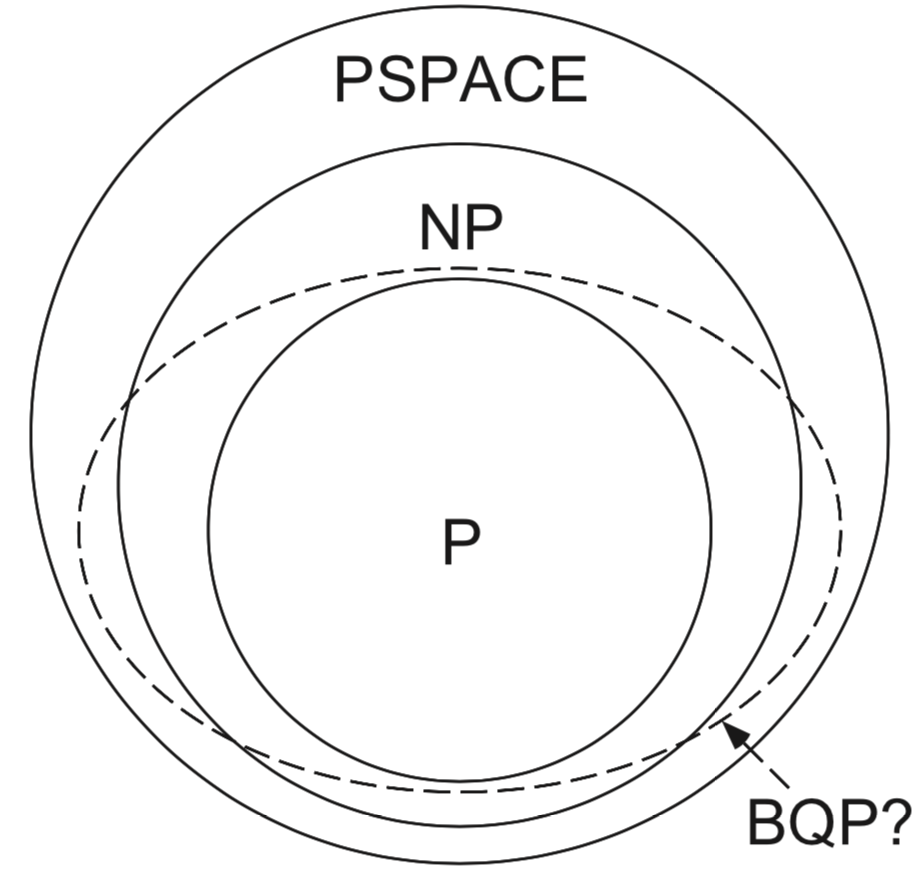
\includegraphics[width=0.75\textwidth]{Figures/BQP_diagram.png}
\caption{A Venn-diagram, illustrating the relationship of $\BQP$ to other classical complexity classes. Figure taken from~\cite{Nielsen2000}.}\label{fig:bqp_venn}
\end{figure}
%Spatial results???
\section{Classical Simulations of Quantum Computation}\label{sec:intro_classical_simulation}
The previous section discussed formal notions of quantum computation, and examined its relation to classical computation through the lens of complexity theory. In this section we will introduce classical simulations of quantum computation. We will begin by introducing more precise notions of classical simulation, before focusing on different classical descriptions of quantum systems. This is by no means an exhaustive survey, but introduces some common paradigms for classical simulation. Finally, we will discuss results on the hardness of classical simulation, and briefly introduce the notion of a `quantum supremacy' test.
\subsection{Definitions of Classical Simulations}\label{sec:intro_simulation_types}
% Types of approximation
% Strong sampling
%  Weak sampling
The general structure of quantum computations involves preparing an initial quantum state $\ket{\va{0}}$, applying a unitary evolution $U$, and then applying a measurement or otherwise estimating an observable. Given this, an obvious definition of classical simulation is to compute the probabilities of different observables on the final state $\ket{\psi}=U\ket{\va{0}}$. This task is typically called `strong' classical simulation~\cite{VandenNest2008}.
\begin{defn}[Strong Classical Simulation]\label{def:strong_simulation}
A strong classical simulator is any classical algorithm $\mathcal{A}$ that takes as input a description of a circuit $U$, and a description of the output observable $s$, and returns the probability of that output $p_{U}\left(s\right)$~\cite{VandenNest2008}.
\end{defn}
Here, $p_{U}\left(s\right)$ could be the probability we observe some $n$-qubit computational state, or a marginal probability obtained by measuring some subset of the qubits. We denote as $\mathbb{S}$ the set of observables we are interested in simulating, and $\mathbb{P}_{\mathbb{S}}$ is the distribution of those events.\par
However, this task is distinct from what we are typically asking a quantum computer to do. When running a quantum algorithm, we are instead preparing the final state $\ket{\psi}$, and then sampling from its output distribution. These samples are then post-processed to estimate other observables. Thus, we introduce the notion of a weak classical simulation.
\begin{defn}[Weak Classical Simulation]\label{def:weak_simulation}
A weak classical simulator is a classical algorithm $\mathcal{A}$ capable of taking a classical description of a circuit $U$, and returning samples from its output distribution $\mathbb{P}_{\mathbb{S}}$~\cite{VandenNest2008}.
\end{defn}
Access to a weak classical simulator should in effect be equivalent to having access to a quantum computer itself~\cite{Pashayan2017}.\par
In practice quantum computations are not perfectly accurate, due to the influence of physical noise and control errors. We can correspondingly relax our definitions of classical simulation, to allow for a degree of approximation. An approximate strong simulation computes a given probability to within some specified precision $\epsilon$, and an approximate weak simulation allows us to sample from a distribution $\mathbb{\hat{P}}_{\mathbb{S}}$ that approximates $\mathbb{P}_{\mathbb{S}}$.\par
There are several different definitions of precision used in approximate classical simulation. For strong simulation, there are three common definitions:
\begin{defn}[Approximate Strong Simulation]\label{def:approximate_strong}
An approximate strong simulator computes estimates of output probabilities $\hat{p}\left(s\right)$ to within a given error $\epsilon$, that is either
\begin{enumerate}
    \item \textbf{Additive}: $\left|p\left(s\right)-\hat{p}\left(s\right)\right| \leq \epsilon\;\forall s\in\mathbb{S}$~\cite{Pashayan2017}
    \item \textbf{Multiplicative}: $\frac{1}{\epsilon}p\left(s\right)\leq \hat{p}\left(s\right) \leq \epsilon p\left(s\right)\;\forall s\in\mathbb{S}$~\cite{Hangleiter2017}
    \item \textbf{Relative}: $\left(1-\epsilon\right)p\left(s\right) \leq \hat{p}\left(s\right) \leq \left(1+\epsilon\right)p\left(s\right) \;\forall s\in\mathbb{S} $~\cite{Hangleiter2017,Bravyi2016}.
\end{enumerate}
\end{defn}
Multiplicative and relative precision are slightly stronger requirements than additive error, as can be seen by considering the case where $p\left(s\right)\rightarrow 0$. In the literature, `relative' simulation is also sometimes referred to as `multiplicative' simulation, as the condition can be rewritten as~\cite{Pashayan2017}
\[\left|p\left(s\right)-\hat{p}\left(s\right)\right| \leq \epsilon p\left(s\right).\]
For weak simulation, the commonly used notion of precision is variously referred to as $\ell_{1}$-precision~\cite{Bremner2011}, additive precision~\cite{Yoganathan2019} or simply $\epsilon$-precision~\cite{Pashayan2017}.
\begin{defn}[Approximate Weak Simulation]\label{def:approximate_weak}
An approximate weak simulator samples from an output distribution $\hat{\mathbb{P}}$ such that
\[ \norm{\mathbb{P}_{\mathbb{S}}-\hat{\mathbb{P}}_{\mathbb{S}}}_{1} = \sum_{s\in \mathbb{S}} \left| p\left(s\right) - \hat{p}\left(s\right)\right| \leq \epsilon.\]
\end{defn}
The one-norm is used as it is directly proportional to the total variational distance between the two distributions.\par
Sometimes, a classical algorithm is capable of generating an approximate simulation $\hat{q}$ with some precision $f\left(\epsilon\right)$, with a non-zero probability of failure such that
\[\text{Pr}\left[\left|q-\hat{q}\right| > f\left(\epsilon\right)\right]\leq \delta.\]
This is referred to as an $\left(\epsilon,\,\delta\right)$-precision approximation~\cite{Pashayan2017}. If the failure probability $\delta$ is bounded, then by $m$ repeat rounds the probability of failure can be reduced to $\delta^{m}$, as in the case for the complexity class $\BPP$.\par
Given these notions then, we can define an efficient $\left(\epsilon,\,\delta\right)$-approximate classical simulation of an $n$ qubit system as one with a complexity that scales as $\poly \left(n, \epsilon^{-1}, \log{\delta^{-1}}\right)$~\cite{Pashayan2017}.
\subsection{Classical Descriptions of Quantum Systems}\label{sec:intro_classical_desc}
% statevector methods & p-blockedness
What could be called the `textbook' description of a quantum computation is the state-vector representation, a vector $\ket{\psi}\in\mathbb{C}^{2^{n}}$ that encodes the wave-function of the $n$-qubit system~\cite{Nielsen2000}. In this picture, the state is updated by applying $2^{n}\times 2^{n}$ unitary matrices. Thus, simulating a quantum computation in this picture might seem to require exponential spatial and temporal resources.\par
However, as quantum circuits are typically built out of local interactions, usually $1$ and $2$ qubit gates, it is possible build block decompositions of both the state-vector and unitary matrices. While a general state-vector requires $2^{n}$ complex numbers to completely specify, a tensor-product of smaller states requires just $O\left(n\right)$~\cite{Ekert1998}.\par
A quantum computation can be described as $p$-blocked if at all time-points it can be decomposed into a tensor product of subsystems each acting on at most $p$ qubits, where $1\leq p\leq n$~\cite{Jozsa2003}. It can be shown that the complexity of both strong and weak classical simulation on a $p$-blocked state-vector has a running time that scales as $O(2^{p+1}\poly\left(m\right))$, where $m$ is the number of blocks~\cite{Jozsa2003}. If $p$ grows at most logarithmically in the system size, then this simulation is efficient. For a fixed $p$, then the runtime also scales efficiently as the system size grows. Otherwise, if $p$ grows unboundedly in the duration of the computation, then simulation requires exponential resources. Interestingly, it can be shown that for example in Shor's algorithm, $p=n$~\cite{Ekert1998}.\par
% Other methods like the binary search trees JMK thingy
The Quantum Multiple Decision Diagram (QMDD) is an alternative encoding of the state-vector that similarly exploits redundancies arising from terms with equal amplitudes~\cite{Niemann2016}. They combine this with a tree-based data-structure, where each leaf of the tree corresponds to a distinct amplitude, labeled by the outcomes to which it corresponds. In general, an arbitrary QMDD will have $2^{n}$ leaves, but the authors show that in practice QMDDs can be significantly smaller than this during common routines including the Quantum Fourier Transform. This can be exploited to develop a classical simulation method where updates scale as $O\left(n \left|v\right|\right)$, where $\left|v\right|$ is the number of leaves in the tree~\cite{Zulehner2017}. If this number grows at most polynomially in the system size, the simulation is efficient.\par
% Approximate QMDD => sparseness, as in VdN
The cases where $\left|v\right|$ grows at most polynomially in the system size corresponds to the definition of computationally tractable states, classes of states that admit efficient strong and weak simulation in the computational basis~\cite{VandenNest2009}. Certain sparse circuits acting on these ``computationally tractable states'' in turn produce a computationally tractable output state, and thus can be efficiently simulated. This definition can also be expanded to approximate simulation, where we approximate its output distribution $\mathbb{P}$ to within additive error $\epsilon$, with some other distribution $\mathbb{\hat{P}}$ that is computationally tractable~\cite{Schwarz2013}.\par
% Tensor network descriptions, alternative picture
An alternative representation of a quantum circuit, that is more distinct from the state-vector picture, is the use of tensor networks to simulate quantum circuits. These methods were first introduced in the context of simulating dynamics of many-body quantum systems~\cite{Vidal2003}.\par
Tensor networks are undirected graphs, where tensors represent input and output states, and quantum gates, and edges represent qubit wires~\cite{Markov2005}. Tensors are combined or contracted by summing over shared indices, with a runtime that scales as the product of the dimensions of the indices to be contracted. For fixed input and output states $\va{x}$ and $\va{y}$, contracting the entire network results in a rank-0 tensor, a scalar value which corresponds to the amplitude $\matrixel{\va{x}}{U}{\va{y}}$~\cite{Markov2005}. It can be shown that the complexity of simulating a tensor network scales exponentially with the `tree-width', a property of the underlying graph of the network~\cite{Markov2005}. In general, tensor networks are known to be efficient when the entanglement of the system is bounded~\cite{Vidal2003}. It can also be shown that for circuits built out of one and two-qubit gates, the tree-width scales linearly with both the number of qubits and the circuit depth~\cite{Markov2005}.\par
% Wigner function picture, born from QO and gaussian states
Yet another alternative classical description of quantum circuits commonly discussed in the literature are quasiprobability or `Wigner function' representations~\cite{Wootters1987}. In this picture, the state is encoded in a quasiprobability distribution on a phase-space, where each point is described by a set of mutually anti-commuting operators~\cite{Wootters1987}. The phase-space can be continuous, as is used in the study of quantum optics~\cite{Nielsen2000}, or discrete, as is usually considered in the context of quantum computing~\cite{Gross2006}.\par
It can be shown that, if the Wigner function representation is strictly positive, then the system is efficiently simulable classically~\cite{Bartlett2002,Mari2012}. This is analogous to the same sign-problem discussed by Feynman in his 1982 address~\cite{Feynman1982}. Positive Wigner function simulations use a random walk across the phase-space, with transition probabilities given by Wigner function expansions of each gate $U$. If the Wigner function is negative, then it is possible to define an alternative sampling strategy that can be used to simulate the computation, but at the expense of an increase in the number of samples, which scales exponentially with the `negativity' of the system, the one-norm of its quasiprobability expansion~\cite{Pashayan2015}. The negativity is by definition $1$ if the system is non-negative, and $>1$ otherwise.
\subsection{Efficiently Simulable Quantum Systems}\label{sec:intro_efficient_simulations}
% Prop D note from Jozsa et al
In the previous section, we briefly introduced several different representations of quantum computations used in classical simulations. In each case, there are also certain circumstances under which the simulation is efficient. Indeed, in their paper on simulation of $p$-blocked computations, it was noted by Jozsa \& Linden that in general for any classical description $\mathcal{D}$, then there exists a corresponding property $\text{prop}\left(\mathcal{D}\right)$ that is required for the simulation to be intractable classically~\cite{Jozsa2003}. For example, in both the $p$-blocked picture and the tensor network picture, the required feature $\text{prop}\left(\mathcal{D}\right)$ is that the entanglement in the system grow unboundedly during the computation~\cite{Jozsa2003,Vidal2003}.\par
% E.g. stabilizer states, explore in detail
Perhaps the most famous example of this requirement is related to the Gottesman-Knill theorem~\cite{Jozsa2003,Gottesman1998b}.
\begin{quote}
\textbf{Gottesman-Knill Theorem:} A quantum circuit built out of only 
\begin{itemize}
    \item Preparation of states in the computational basis
    \item Clifford and Pauli gates
    \item Measurement in the computational basis
\end{itemize}
can be efficiently simulated on a classical computer.
\end{quote}
We will discuss the Gottesman-Knill theorem and how these circuits, typically called stabilizer circuits, can be simulated in Chapter~\ref{chap:stabilizers}.\par
This theorem has gained particular attention in the field for several reasons. Firstly, it sets up a clear correspondence between classical simulability and universal quantum computing. The gate-set of stabilizer circuits is not universal for quantum computation. This means these circuits cannot be used to build up arbitrary unitary operations~\cite{Nielsen2000}. In fact, stabilizer circuits are also not universal for classical computation~\cite{Aaronson2004}. However, introducing a single gate outside of this set is sufficient to generate a group dense in the special unitary group, and thus `promote' the gate-set to universality. These universal circuits are in turn no longer efficiently simulable.\par
Stabilizer circuits are also closely related to the study of quantum error-correcting codes, where logical gates `native' to the code are typically Pauli and Clifford gates corresponding to stabilizer circuits~\cite{Nielsen2000}. Non-Clifford gates are then introduced through a protocol called state-injection, involving `magic' states that cannot be generated by stabilizer circuits~\cite{Gottesman1999,Bravyi2005}.\par
Interestingly, it has also been shown that there is a correspondence between stabilizer circuits, and `contextuality', a generalised notion of locality~\cite{Howard2014}. Contextuality was first discussed in the 1960s, where it was argued that non-contextuality is a unique feature of quantum systems~\cite{Bell1966,Kochen1967}. For example, in Spekkens's Toy Model ~\cite{Kochen1967}, a classical model of quantum systems based on a restriction of available information, features like non-locality and entanglement can be efficiently described, but contextuality cannot. Similarly, it was shown by Howard et al.\ that in odd-prime dimensional quantum systems, stabilizer circuits are entirely non-contextual, and the onset of contextuality is connected to the ability to distill high-fidelity magics states~\cite{Howard2014}. The case is slightly more complicated for quantum computing with qubits, as qubits show state-independent contextuality, but recent work has explored this correspondence between contextuality and qubit magic states~\cite{BermejoVega2017}.
\subsubsection{Resources for Quantum Computation}
% Prod D and resources
The Gottesman-Knill theorem makes it clear that non-stabilizer resources are required for universal quantum computation, and as stated there is a correspondence between this required property and classical simulability. In fact, in general, the property $\text{prop}\left(\mathcal{D}\right)$ can be interpreted as `required' for quantum advantage, from the corresponding breakdown of efficient classical simulation. Jozsa \& Linden argue that rather than any one `true' $\text{prop}\left(\mathcal{D}\right)$, it is likely that any quantum computation with quantum advantage requires all of these properties to be true.\par
% Examples
For example, as discussed in the $p$-blocked case, this suggests that entanglement is required for quantum advantage. However, given that entangled stabilizer circuits exist, entanglement alone is clearly not sufficient. Similarly however, it is easy to construct non-stabilizer circuits that are either $p$-blocked, or sparse such that the output is computationally tractable.\par
The study of these potential resources, not only for computation but also for non-classical phenomena more generally, are called quantum resource theories. In general, a quantum resource theory is composed of a set of states that are considered `free', a set of states that have an associated `cost', and a set of allowed or `free' operations~\cite{Brandao2015}. We are then interested in asking what is the associated resource cost of certain protocols, and how does the resource behave under free operations?\par
Resource theories have been applied to a broad range of phenomena, including; non-stabilizer states~\cite{Veitch2014}; magic states~\cite{Howard2017}, more specifically; and asymmetry~\cite{Piani2016}, which relates to both computational tractability~\cite{VandenNest2009} and to generalizations of Gottesman-Knill called normalizer circuits~\cite{BermejoVega2014}. Of particular interest are resource theories where the set of free states is convex, as these also admit convex cost functions that can be more easily analysed~\cite{Regula2018}. All of the examples given in this paragraph fall into the category of convex resource theories~\cite{Chitambar2019}.\par
% Simulation schemes w/ wigner function
There is also typically a correspondence between free states and operations in resource theories and their classical simulability. Indeed, many of the resource theories discussed above explicitly admit classical simulation through a discrete Wigner function representation. For example, it can be proven that any mixed state on $n$ qubits with a positive Wigner function representation can be described as a convex mixture of stabilizer states~\cite{Gross2006}. In these pictures, the resource cost of a given state is directly related to the computational cost of classical simulation~\cite{Howard2017,Kocia2017,Seddon2019,Raussendorf2019}.\par
As an example of the power of resource theories, we can consider the Robustness of Magic (RoM), introduced in~\cite{Howard2017}. This measure is equal to the negativity of a stabilizer state decomposition of a state. The RoM is largest for pure, non-stabilizer states, which lie outside the convex hull of the stabilizer states. However, as the state we are considering becomes more and more mixed, for example as a result of environmental noise, it is pushed closer to the set of free states. Below some threshold, the state has RoM $\mathcal{R}\left(\rho\right)=1$, and can be efficiently simulated. This corresponds neatly with the notion of magic state distillation, where we are trying to `distill' pure magic states using Clifford circuits. We are consuming multiple copies to produce a magic state with increased robustness, which are subsequently harder to classically simulate and more useful for quantum computing. It is also congruous with the existence of a noise threshold below which we cannot distill any magic state~\cite{Bravyi2005}; below this threshold, the `noisy' magic states are `free' states, and thus we cannot increase their RoM using just free operations.
%TODO: Add figure???
\subsection{Simulation and Quantum Advantage}\label{sec:intro_complexity}
Given some of the results quoted in the previous sections, we might imagine that with continued development a sufficiently optimized classical method could exist to simulate quantum circuits. Here, we will review results from complexity theory which suggest that even an approximate efficient classical simulation of arbitrary quantum computation should not be possible.\par
\subsubsection{Hardness of Strong Simulation}
% Hardness of strong simulation
% Encodes #P
It can be shown that exact strong simulation would imply the existence of efficient classical algorithms to solve problems in $\#\P$, using a correspondence based on quantum circuits. From a famous computational result in complexity theory called Toda's theorem, it can be shown that the complexity class of problems solvable by a $\P$ algorithm with access to an oracle for $\#\P$, typically denoted $\P^{\#\P}$, in fact contains the entire $\PH$~\cite{Toda1991}. Thus, the existence of an efficient classical algorithm for $\#\P$ problems would imply even stronger consequences than $\P=\NP$.\par
The proof relies on the ability to construct quantum circuits $C$ out of $H$ and Toffoli gates~\cite{Dawson2004}, or alternatively out of $H$, $Z$, $CZ$ and $CCZ$ gates~\cite{Montanaro2017}, such that computing the probability amplitude 
\[\matrixel{\va{0}}{C}{\va{0}} \propto \text{gap}\left(f\right),\]
where $f\,:\,\{0,1\}^{n}\rightarrow \{0,1\}$ is an $n$-variable binary polynomial, and
\[\text{gap}\left(f\right) = [\# \va{x}:f\left(\va{x}\right)=1] - [\# \va{x}:f\left(\va{x}\right)=0].\]
Computing the gap of a cubic polynomial is known to be $\#\P$ hard in general, if $f$ has degree $\geq 3$~\cite{Montanaro2017}, and thus could be efficiently solved by an efficient strong simulation.\par
Interestingly, this example also illustrates a case where studying quantum algorithms casts light on classical complexity theory. It was believed but not conclusively shown that $\text{gap}\left(f\right)$ could be efficiently computed for polynomials with degree $\leq 2$. A quantum circuit to compute the gap of such a polynomial could be built using just $H$, $Z$, and $CZ$ gates, and is thus a stabilizer circuit. This means the amplitude $\matrixel{\va{0}}{C}{\va{0}}$ can in turn be computed efficiently, resolving the open problem~\cite{Montanaro2017}. This example also further illuminates the relationship between universal quantum circuits and classical computation; circuits built using $H$, $Z$, $CZ$ and $CCZ$ gates are known to be universal for quantum computing, and in turn are likely not to be strongly simulable.\par
% Hard to even approximate
% Relation to Ising Partition Funtions, matrix permanent
There is in fact evidence that even approximate strong simulation of quantum computations would also imply the collapse of the $\PH$.
For example, there exists a $\BQP$ algorithm for approximately evaluating the Jones polynomial~\cite{Aharonov2007}, an important problem in the study of topological quantum field theories, to within additive error. This algorithm is based on repeatedly running a quantum circuit a polynomial number of times to obtain an estimate of a particular amplitude, and thus a strong classical simulation could be used to compute the Jones polynomial exactly. However, it can be shown that even approximating the Jones polynomial to within multiplicative error $\epsilon$ is a problem in $\#\P$~\cite{Kuperberg2009}, and thus no approximate strong classical simulation can exist unless the $\PH$ collapses. Interestingly, it is believed that approximately evaluating the Jones polynomial is a $\BQP$-complete problem, and thus this result would suggest that $\BQP$ problems cannot be efficiently strongly simulated classically.\par
A core lemma in the proof of~\cite{Kuperberg2009} is that given some family of quantum circuits $C$ such that the class of problems solvable by $C$ circuits under postselection $\mathbf{postC}=\PostBQP$, then an efficient strong simulation of the output distribution of $C$ would collapse the polynomial hierarchy. For the algorithm for the Jones polynomial, this follows naturally as the problem is $\BQP$-complete. Interestingly however, this result can also be used to imply that approximate strong simulation is hard even for certain types of quantum computation that are `weaker' i.e.\ they are strictly not universal~\cite{Aaronson2010}. For example, Instantaneous Quantum Polynomial (IQP) circuits, circuits with depth $\poly\left(n\right)$, built out commuting gates like $Z$, $CZ$ and $CCZ$, have the property that they are universal under post-selection~\cite{Bremner2011}. Thus, strong simulation of IQP circuits implies the collapse of the $\PH$~\cite{Goldberg2014}.\par
An alternative strategy involves finding some correspondence between the quantum computation and another problem known to be $\#\P$ hard. For example, the output distribution of IQP circuits can be shown to be equivalent to partition functions of Ising model Hamiltonians~\cite{Fujii2017}, and thus from a characterisation of these partition functions IQP circuits are $\#\P$ hard to simulate in general~\cite{Goldberg2014}. This is also the strategy employed by Aaronson \& Arkhipov, when showing that a quantum optics task called Boson Sampling is equivalent to computing the permanent of a matrix to within additive error~\cite{Aaronson2010}, a known $\#\P$-hard problem~\cite{Valiant1979}.
% Acceptance probability?quant-ph/9812056
\subsubsection{Extending Results to the Weak Simulation Case}
% Van den Nest, separation between strong and weak sampling
While the results above apply to strong classical simulation, as discussed weak simulation can be considered as a more appropriate definition of classical simulation. It was also shown by Van den Nest that it is possible to construct quantum circuits whose strong simulation can be proven to be in $\#\P$, but which nonetheless admit an efficient weak simulation~\cite{VandenNest2008}. Thus, a bound on strong simulation is not sufficient to rule out classical simulation of quantum circuits.\par
Initial evidence for the hardness of weak sampling was given in~\cite{Bremner2011}, where the authors showed a weak simulation of IQP circuits with multiplicative error would imply the collapse of $\PH$. Here, multiplicative error means that we have some approximate distribution $\hat{\mathbb{P}}$, such that every term is itself a multiplicative approximate of the true probability. This is a strong requirement for approximate classical simulation.\par
% Connecting approximate strong and weak computation
Subsequent work has shown that in fact, it is possible to lift a complexity theoretic bound on strong simulation with multiplicative error, to obtain an equivalent bound on weak simulation with additive error, given a proof that the circuit families satisfies a pair of conjectures called `anti-concentration' and `average-case hardness'~\cite{Hangleiter2017}. Recall that we are considering a family of quantum circuits $C$, which are hard to approximately strongly simulate, either as they are universal under postselection, or through correspondence to some other problem which is known to be $\#\P$-hard in the worst case.\par
The output distribution of these circuits is said to anticoncentrate if there exist two positive real numbers $\alpha$ and $\beta$, such that
\begin{equation}
\text{Pr}_{U\sim \mathbb{P}_{C}}\left(\left|\matrixel{\va{x}}{U}{\va{0}}\right|^{2}\geq \frac{\alpha}{N}\right) > \beta,
\label{eq:anticoncentration}
\end{equation}
where $N$ is the dimension of the system, typically $2^{n}$ for $n$ qubits~\cite{Hangleiter2017}. This inequality states that for some random circuit $U$ drawn from the family $C$, the probability of an arbitrarily chosen entry being greater than uniform is greater than $\beta$. Intuitively, anticoncentration requires that there is high probability the output distribution of $U$ is reasonably close to uniform~\cite{Harrow2017}. This ensures we are unlikely to find a circuit $U$ with an exactly or approximately sparse output distribution, that would be subsequently amenable to classical simulation~\cite{VandenNest2008,Schwarz2013}.\par
Average-case hardness requires that, given a problem that is known to be $\#\P$ hard to approximately compute in the worst-case, then it is also $\#\P$ hard to simulate on some constant fraction $c>0$ of the problem instance~\cite{Bremner2016}. This takes us from a family of problems that can in principle be hard to simulate, to one where there are many instances known to be hard to simulate~\cite{Harrow2017}. For example, some Ising Hamiltonians, and thus some instances of IQP circuits, are known to be classically simulable~\cite{Fujii2017}. Nonetheless, IQP circuits can be shown to satisfy average-case hardness~\cite{Bremner2016}.\par
These two properties can be combined with a result from classical complexity theory called the Stockmeyer Counting Algorithm~\cite{Stockmeyer1985}. Taken together, average-case hardness and anticoncentration imply that a classical simulator capable of sampling from the output distribution with a worst-case additive error, is in fact capable of sampling with an average-case multiplicative error~\cite{Bremner2016}. Subsequently, using the Stockmeyer algorithm, this weak simulator can then be used to obtain an estimate of an output probability with multiplicative error. This completes the reduction from weak simulation with additive error, to strong simulation with multiplicative error, and thus shows that weak simulation is also $\#\P$-hard~\cite{Bremner2016}.\par
% Hakop paper about connecting estimating probabilties and sampling
% Polybox notion, strong additive approximation also insufficient for efficient sampling
Subsequent work has strengthened the case for the hardness of weak simulation. Consider having access to a classical algorithm capable of computing certain output probabilities with additive $\left(\epsilon,\delta\right)$-precision, efficiently --- namely, with a runtime that scales as $\poly\left(n,\epsilon^{-1},\log\delta^{-1}\right)$. Such a device is called a poly-box~\cite{Pashayan2017}. It can be shown that even with such a capability, the output distribution cannot be efficiently weakly simulated with additive error as long as the output distribution $\mathbb{P}$ is not approximately sparse. Namely, there does not exist some distribution $\hat{\mathbb{P}}$ such that $\norm{\mathbb{P}-\mathbb{\hat{P}}}\leq \epsilon$, and which has $t=\poly\left(\epsilon^{-1}\right)$ non-zero amplitudes. In other words, even with such a strong classical simulation device, the distribution cannot be weakly simulated if it is sufficiently dense.
\subsubsection{Quantum `Supremacy'}
% Connection to quantum supremacy experiments
While not necessarily practically applicable, these kind of random problems that are believed to be hard to simulate clasically under the assumption the $\PH$ does not collapse form the basis of an effort in the quantum computing community to demonstrate so-called `quantum supremacy' --- the ability for a quantum computer to successfully run an algorithm super-polynomially faster than a classical computer~\cite{Preskill2012}.\footnote{I want to acknowledge here the very real concerns that have been raised about the use of the word supremacy, given the historical and contemporary political significance of the word. I use the term in this thesis as, despite much discussion, it has become the \emph{de facto} name for this phenomenon.}
\par
Random circuit problems are especially interesting compared to more direct tasks such as Shor's algorithm, because they require significantly fewer qubits to implement, and in some cases do not even require a universal architecture~\cite{Montanaro2017}. They also have much stronger guarantees on their computational hardness compared with `analogue' quantum simulators, quantum systems that realise model Hamiltonians~\cite{Montanaro2017}. That said, there has also been recent effort in the community towards constructing quantum simulators with provable hardness~\cite{Hangleiter2017,Gao2017,BermejoVega2018,Haferkamp2019}.\par
A quantum supremacy experiment based on these kind of random sampling problems with be made up of two key parts: sampling, and verification. The first task, also referred to as `Heavy Output Generation', is to generate a large number of samples from the output distribution of a given quantum circuit, drawn at random from a family of circuits~\cite{Aaronson2016}. This is done simultaneously using both a quantum computer, and an appropriate classical simulation method, presumably using High Performance Computing (HPC) resources.\par
The next step is to use an additional classical method to verify the output of both the quantum and classical samples. This step is in general even more computationally intensive than the sampling step, and is a significant caveat in current quantum supremacy proposals compared to running an $\NP$ problem such as factorization, which can be efficiently checked~\cite{Harrow2017}. After verification, the runtime and resources required for both the quantum and classical methods are compared.\par
An important caveat in realising quantum supremacy experiments, however, is their susceptibility to noise. As previously discussed, sufficiently noisy quantum computations can in fact be efficiently simulated classically. It is thus important that quantum supremacy protocols are reasonably robust, as quantum error correction is out of reach for contemporary quantum computers~\cite{Preskill2018}.\par
This caveat also acts in tandem with continued development of classical simulation methods. For example, recent effort in simulation of noisy boson sampling problems has pushed the threshold for quantum supremacy to around $30-40$ photons~\cite{Neville2017}, compared to current experimental records of about $6$.\par
Because noisy quantum circuits can typically be more easily simulated, an alternative proposal for quantum supremacy experiments changes the order of the classical sampling and verification steps. The idea is to use a classical verifier capable of estimating noise in the system~\cite{Villalonga2019}, such that this noise parameter can be used as input to the classical simulation to enable a fairer comparison.


% !TEX root = ../Main.tex

\chapter[Methods for Simulating Stabilizer Circuits]{Methods for Simulating Stabilizer\\ Circuits}
\label{chap:stabilizers}

\section{Introduction}\label{sec:stabilizer-intro}
% Stabilizer circuits are an intersting class of circuits
% Capture many seemingly quantum features
% Recap definition
% Some of this is probably meant for intro instead
In the previous chapter (INSERT REFERENCE), we briefly introduced the notion of stabilizer circuits as a class of efficiently simulable quantum computations. In this chapter, we revisit stabilizer circuits in detail, with a focus on different classical data structures for encoding stabilizer states and the corresponding algorithms for simulations.\par
Several informal definitions of stabilizer circuits have been used in the quantum computing literature~\cite{Gottesman1998b,Aaronson2004,VandenNest2008,Seddon2019}. However, what each definition has in common is that the operations $\mathcal{E}$ acting on an abelian subgroup $\mathcal{S} \subseteq \mathcal{P}_{n}$ generate a new subgroup $\mathcal{S'}\subseteq \mathcal{P}_{n}$. These groups $\mathcal{S}$ are also called a stabilizer groups.\par
In this thesis, we focus exclusively on stabilizer circuits acting on pure states $\ket{\phi}$ called stabilizer states. These can be entirely characterized by their associated stabilizer group as
\begin{equation}
    s\ket{\phi}=\ket{\phi}\;\forall s\in\mathcal{S}
\end{equation}
For an $n$-qubit state, the group $\mathcal{S}$ has $2^{n}$ elements~\cite{Gottesman1998b}. As $\mathcal{S}$ is also abelian, this means it can be described by a generating set with $n$ elements,
\begin{equation}
    \mathcal{S} = \langle g_{1}, g_{2},\dots,g_{n}\rangle \; : g_{i}\in\mathcal{S},
\end{equation}
which are commonly referred to as the `stabilizers' of the state $\ket{\phi}$. We also note that this definition allows us to write
\begin{equation}
    \ketbra{\phi} = \frac{1}{2^{n}}\sum_{s\in\mathcal{S}} s = \frac{1}{2^{n}}\prod_{i=1}^{n}\left(\mathbb{I}+g_{i}\right)
\end{equation}
Given that these circuits map stabilizer states to other stabilizer states, this means they must be built up of unitary operations $U$ which map Pauli operators to other Pauli operators under conjugation. This set is commonly denoted as $\mathcal{C}_{2}$, or the `second level of the Clifford hierarchy' 
\begin{align}
    \mathcal{C}_{2} &\equiv \{U\,:\,UPU^{\dagger}\in\mathcal{P}_{n}\;\forall P\in\mathcal{P}_{n}\} \label{eq:c2}\\
    \mathcal{C}_{j} &\equiv \{U\,:\,UPU^{\dagger}\in\mathcal{C}_{j-1}\;\forall P\in\mathcal{P}_{n}\} \label{eq:cj}
\end{align}
where in Eq.~\ref{eq:cj} we have also introduced the (recursive) definition for level $j$ of the Clifford hierarchy. From this definition
\begin{equation}
    V\mathcal{S}V^{\dagger}=\langle Vg_{i}V^{\dagger}\rangle = \langle g_{i}' \rangle = \mathcal{S}'
\end{equation}
%TODO: Do we need to explain measurement or just cite it? Maybe this comes up later in the implementation...
We also allow stabilizer circuits to contain measurements in the Pauli basis~\cite{Gottesman1998b}.
\subsubsection*{Simulating stabilizer circuits}
% Classical simulabiltiy follows from gate updates and encoding
% Introduce tableaux, and classical encoding
From the above definitions, we can see that simulating a stabilizer circuit on $n$ qubits corresponds to updating the $n$ stabilizer generators for each unitary and measurement we apply. As the number of generators grows linearly in the number of qubits, if these group updates can be computed in time $O\left(\poly (n)\right)$ then it follows the circuits can be efficiently simulated clasically.\par
The first proof of this was given by Gottesman in \cite{Gottesman1998b}, by showing through examples that stabilizer updates can be quickly computed for the CNOT, H and S gates, and for single qubit Pauli measurements. This is significant as the $n$ qubit Clifford group can be entirely generated from these gates.
\begin{equation}
    \mathcal{C}_{2} = \langle CNOT_{i,j},\, H_{i},\, S_{i}\,:i,j\in \mathbb{Z}_{n}\rangle. \label{eq:cliffordgen}
\end{equation}
This result is typically referred to as the `Gottesman-Knill' theorem.\par
A more formal proof follows from the work of Dehaene \& de-Moor, who showed that the action of Clifford unitaries on Pauli operators corresponds to multiplication of $(2n+1)\times (2n+1)$ symplectic binary matrices with $(2n+1)$-bit binary vectors~\cite{Dehaene2003}. The dimension of these elements also grows just linearly in the number of qubits, and as matrix multiplication requires time $O(n^{2.37})$ it follows that we can update the stabilizers in $O(mn^{2.73})$ for $m$ Clifford gates.\par
This work was then extended by Aaronson \& Gottesman, who introduced an efficient data structure for stabilizer groups, and algorithms for their updates under Clifford gates and Pauli measurement~\cite{Aaronson2004}. This method avoids the need for matrix multiplications, instead providing direct update rules allowing stabilizer circuits to be simulated in $O(n^{2})$.\par
Since 2004, there have been several papers looking at different data structures and algorithms for simulating stabilizer circuits of the type we consider here. For example, a method based on encoding stabilizer states as graphs~\cite{Anders2006}, refinements of the Aaronson \& Gottesman encoding~\cite{Garcia2012}, and an encoding using affine spaces and phase polynomials~\cite{VandenNest2008,Bravyi2016}.\par
In the rest of this section, we will discuss different aspects of simulating stabilizer circuits, focusing on updating stabilizer states under gates and measurements, computing stabilizer inner products, and the connections between stabilizer circuits and states.
% \clearpage
\subsection{Tableau Encodings of Stabilizer States}\label{sec:sympencoding}
The method in \cite{Aaronson2004} is based on a classical data structure they call the `stabilizer tableau', a collection of Pauli matrices that define the stabilizer group, encoded using the binary symplectic representation of \cite{Dehaene2003}
\begin{equation} P = i^{\delta}-1^{\epsilon} \bigotimes_{i=1}^{n} x_{i}z_{i}\end{equation}
where the Pauli matrix at qubit $i$ is defined by two binary bits such that
\begin{equation}
    x_{i}z_{i} = \begin{cases}
    I & x_{i}=z_{i}=0\\
    X & x_{i}=1, z_{i}=0 \\ 
    Z  &x_{i}=0, z_{i}=1 \\
    Y  &x_{i}=z_{i}=1
    \end{cases}
\end{equation}
Together with the $\delta$ and $\epsilon$ phases, a generic Pauli operator can be encoded in $2n+2$ bits; two bits to encode the phase, and two $n$-bit binary strings $\tilde{x},\tilde{z}\in\mathbb{Z}_{2}^{n}$ to encode the Pauli acting on each qubit, commonly referred to as `x-bits' and `z-bits' respectively. In this picture, multiplication of Pauli operators corresponds to addition of $x$ and $z$ bits modulo 2, with some additional, efficiently computable function for correcting the phase~\cite{Dehaene2003}
\begin{align}
    P Q &= i^{\delta_{pq}}-1^{\epsilon_{pq}}\bigotimes_{i=1}^{n}x_{i}' z_{i}' \\
    x'_{i} &= x_{pi}\oplus x_{qi} \\
    z'_{i} &= z_{pi} \oplus x_{qi}
\end{align}
where $\delta_{pq} = \delta_{p}\oplus \delta_{q}$, $\epsilon_{qr} = f(\tilde{x}_{p}, \tilde{z}_{p}, \tilde{x}_{q}, \tilde{z}_{q})$.\par
%%Tableau definition, drops an extra factor of n bits
%% Gate updates
In stabilizer groups, we can restrict ourselves to considering Pauli operators with only real phase. This is because if $iP\in\mathcal{S}$, then $(iP)^{2}=-I\in\mathcal{S}$. But, this implies that $-I\ket{\phi}=\ket{\phi}$, which is a contradiction.\par
While only $n$ generators $S_{i}$ are needed to characterize the stabilizer group $\mathcal{S}$, the tableau also includes an additional $2n$ operators called `destabilizers' $D_{i}\in\mathcal{P}_{n}$. Together, these $2n$ operators generate all $4^{n}$ elements of $\mathcal{P}_{n}$.\par
There are many possible choices of destabilizer, but the tableau chooses operators such that~\cite{Aaronson2004}
\begin{align*}
    \comm{D_{i}}{D_{j}} &= 0\;\forall\, i, j \,\in \{1,\dots,n\} \\
    \comm{D_{i}}{S_{j}} &= 0 \iff i\neq j \\
    \acomm{D_{i}}{S_{i}} &= 0 
\end{align*}
Altogether, the full tableau has spatial complexity $4n^{2}+2n$. These are sometimes referred to as `Aaronson-Gottesman 'tableaux or `CHP' tableaux, after the software implementation by Aaronson~\cite{Aaronson2004b}.
\begin{figure}[H]
\begin{equation}
\kbordermatrix{~ & ~ & ~ & ~ & ~ & ~ & ~ & ~ & ~ & ~\\
    \mathcal{D}_{1} & x_{1,1} & \cdots & x_{1,n} & \omit\vrule & z_{1,n} & \cdots & z_{1,n} & \omit\vrule & r_{1} \\
    \vdots & \vdots & \ddots & \vdots &\omit\vrule & \vdots & \ddots & \vdots & \omit\vrule  &\vdots \\
    \mathcal{D}_{n} & x_{n,1} & \cdots & x_{n,n} & \omit\vrule & z_{n,1} & \cdots & z_{n,n} & \omit\vrule & r_{n}\\ \hline
    \mathcal{S}_{1} & x_{n+1,n} & \cdots & x_{n+1,n} & \omit\vrule & z_{n+1,1} & \cdots & z_{n+1,n} & \omit\vrule & r_{n+1}\\
    \vdots & \vdots & \ddots & \vdots & \omit\vrule & \vdots & \ddots & \vdots & \omit\vrule & \vdots \\
    \mathcal{S}_{n} & x_{2n, 1} & \cdots & x_{2n, n} & \omit\vrule & z_{2n,1} & \cdots & z_{2n,n}&\omit\vrule&r_{2n}
    }
\end{equation}
\caption{Example of a `CHP' tableau, where the first $n$ rows are the Destabilizers and the next $n$ rows are the stabilizers. The $2n+1$th column gives that phase $-1^{r_{i}}$ for each operator.}
\label{fig:ExampleCHP}
\end{figure}
\subsubsection*{Simulating Gates}
Gate updates for each individual operator in the tableau can be computed constant time. For example, the Hadamard transforms single qubit Pauli matrices under conjugation as
\begin{equation}
    HPH^{\dagger} = \begin{cases}
        I & P=I\\
        Z & P=X\\
        X & P=Z\\
        -Y & P=Y
        \end{cases}
\end{equation}
In the symplectic form, we then have to update the $i$th Pauli operator as
\begin{equation}
    x_{i}'z_{i}' = (x_{i}\oplus p)(z_{i}\oplus p) \; : \; p = x_{i} \oplus z_{i}
\end{equation}
and the phase as
\begin{equation}
\delta' = \delta \oplus \left(x_{i}\wedge z_{i}\right)
\end{equation}
Similar update rules exist for the CNOT and S gates, which together generate the $n$ qubit Clifford group. As there are $O(n)$ operators in the tableau, and each update is constant time, gate updates overall take $O\left(2n\right)$~\cite{Aaronson2004}. This is in contrast to the $O(n^{2.37})$ complexity of~\cite{Dehaene2003}
\subsubsection*{Simulating Measurements}
The addition of the destabilizer information is  used to speed up the simulation of Pauli measurements on Stabilizer states. Measuring some operator $P$ on a stabilizer state will always produce either a deterministic outcome, or an equiprobable random outcome~\cite{Gottesman1998b}.\par
If the outcome is deterministic, then $\pm P$ is in the stabilizer group, and the outcome is $+1$ or $-1$ respectively. Using the stabilizer genereators, this allows us to write 
\begin{equation}
    \comm{P}{S_{i}}=0\;\forall S_{i}\in\mathcal{S} \implies \prod_{i}c_{i}S_{i} = \pm P. \label{eq:det_requirement}
\end{equation}
for binary coefficients $c_{i}$.\par
Checking if the outcome is deterministic takes $O(n^{2})$ time in general, using the symplectic inner product to check the commutation relations~\cite{Dehaene2003}. However, checking which measurement outcome occurs involves computing the coefficients $c_{i}$. In the symplectic form, thiscan be rewritten as
\[
    Ac=P
\]
where $c$ is a binary vector, $A$ is a matrix with each stabilizer as a column vector, $P$ is the operator to measure, and we have dropped the phase. Solving this would require inverting the matrix $A$, and take time $O(n^{3})$.\par
Aaronson \& Gottesman show that for single qubit mesurements, including destabilizer information instead allows us to compute the $c_{i}$ and the resulting measurement outcome in $O(n^{2})$. As this is a single qubit measurement, they also show that the commutivity relation requries checking only individual bits of the stabilizer vectors, also reducing that step to $O(n)$ time.\par
For random measurements, from Eq.~\ref{eq:det_requirement}, $\exists S_{i}:\acomm{S_{i}}{P}=0$, and it suffices to replace this stabilizer with $P$, and update the other elements of the group as $S_{j}'=PS_{j}$ iff $\acomm{S_{j}}{P}=0$~\cite{Gottesman1998b,Aaronson2004}.
\subsubsection*{`Canonical' Tableaux}
% A&G fix tableaux through initial state
There are multiple possible choices of generators for each stabilizer group/state. For example, for the Bell state $\ket{\phi^{+}}=\frac{1}{2}\left(\ket{00}+\ket{11}\right)$
\begin{align}
    \mathcal{S} = \{II, XX, -YY, ZZ\} = \langle XX,-YY\rangle = \langle XX, ZZ\rangle = \langle -YY,ZZ\rangle.
\end{align}
In simulation, tableau are fixed by choice of a convention. For example, it is possible to arrive at a `canonical' set of stabilizer generators using an algorithm which strongly resembles Gaussian elimination~\cite{Garcia2012}. This method rearranges the stabilizer rows of the tableau by multiplying and swapping generators, such that the overall stabilizer group is left unchanged. Computing this canonical form requires  time $O(n^{3})$~\cite{Garcia2012}.
\begin{figure}[H]
    \centering
    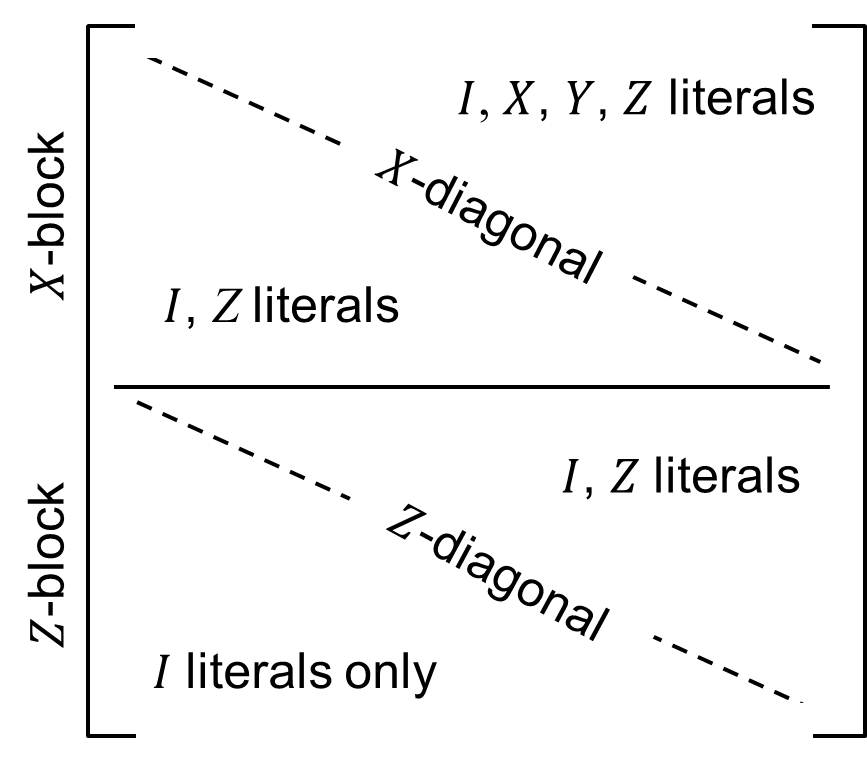
\includegraphics[width=0.45\linewidth]{stbmtx_inv.jpg}
    \caption{Representation of the canonical or `row-reduced' set of stabilizer generators. Figure taken from~\cite{Garcia2012}.}
\label{fig:canoncialtableau}
\end{figure}
These tableau can then be updated using the same methods as in \cite{Aaronson2004}, though this will in general not preserve the canonical form. Each Clifford gate will change one or two columns of the tableau, and thus an additional $O(n)$ row multiplications are required to restore it to canonical form, taking total time $O(n^{2})$ per gate~\cite{Garcia2015}.
Importantly this canonical tableau can also be used to compute deterministic measurement outcomes in time $O(n)$, and so this method can simulate measurement outcomes more efficiently at the cost of more expensive gate updates~\cite{Garcia2015}.\par
In contrast, Aaronson \& Gottesman fix the stabilizer tableau through an initial state, $\ket{0}^{\otimes n}$. The full tableau for this state looks like the identity matrix, with an additional zero-column for the phases. The tableau of a given state $\ket{\phi}$ is then built-up gate by gate using a stabilizer circuit $V:\ket{\phi}=V\ket{0^{\otimes n}}.$
\subsection{Connecting Stabilizer States and Circuits}
% Connection between clifford circuits and states
The convetion for `CHP' stabilizer tableaux mentioned above, and the definition of stabilizer circuits given in Section~\ref{sec:stabilizer-intro}, show that stabilizer states can also be defined by a stabilizer circuit and an initial state.\par
In \cite{Aaronson2004}, the authors derive examples of these `canonical circuits', and show that its possible for any stabilizer state to be synthesised by a unique circuit acting on the $\ket{0^{\otimes n}}$ state
\begin{equation}
    \ket{\phi} = V\ket{0} = H\;C\;S\;C\;S\;C \;H \; S \;C \;S \ket{0^{\otimes n}}\label{eq:chpcirc}
\end{equation}
where each letter denotes a layer made up of only Hadamard (H), CNOT (C) or S gates. The proof is based on  a sequence of operations reducing an arbitrary tableau to the identity matrix, each step of which corresponds to applying layers of a given Clifford gate~\cite{Aaronson2004}. As a corollary, the total number of gates in the canonical circuit for an $n$-qubit stabilizer state scales as $O(n\log (n))$~\cite{Aaronson2004}, based on previous work on synthesising $CNOT$ circuits with the $O(n\log (n))$ gates~\cite{Patel2003}, and that each $H$ and $P$ layer can act on at most $n$-qubits.\par
A slightly simpler canonical form was derived in 2008, which allows a stabilizer circuit to be written as
\begin{equation}
    \ket{\phi} = S\;CZ\;X\;C\;H \ket{0^{\otimes n}} \label{eq:affinecirc}
\end{equation}
where the CZ and X layers are made up of Controlled-Z gates and Pauli X gates, respectively~\cite{VandenNest2008}. This circuit follows from the work of \cite{Dehaene2003}, who showed that any stabilizer state can be written as
\begin{equation}
    \ket{\phi} = \frac{1}{\sqrt{2^{k}}}\sum_{x\in\mathcal{K}} i^{f(x)}\ket{x}.\label{eq:affineform}
\end{equation}
In this equation, $\mathcal{K}\subseteq\mathbb{Z}_{2}^{n}$ is an affine subspace of dimension $k$, and $f(x)$ is a binary  function evaluated $\bmod\,4$. Thus, a stabilizer state is always a uniform superposition of computational basis strings, with individual phases $\pm \mathi,\,\pm 1$. The affine space $\mathcal{K}$ has the form
\[
    \mathcal{K}=\{Gu + h\}
\]
for $k$-bit binary vectors $u$, an $n\times k$ binary matrix G, and an $n$-bit binary `shift-vector' $h$.\par
Van den Nest notes that this representation can be directly translated into a stabilizer circuit; we begin by applying $H$ to the first $k$ qubits to initialize the state $\sum_{u}\ket{u}\otimes\ket{0^{\otimes n-k}}$. We then apply CNOTs to prepare $\sum_{u}\ket{Gu}$, and finally Pauli Xs to preapre $\sum_{u}\ket{Gu\oplus h}$~\cite{VandenNest2008}.\par
The phases can be further decomposed into two linear and quadratic binary functions $l,q\,:\mathbb{Z}_{2}^{n}\rightarrow\mathbb{Z}_{2}$, such that $i^{q(x)}=i^{l(x)}(-1)^{q(x)}$. The linear terms correpsond to single qubit phase gates, which can be generated by the S gate, and the quadratic terms to two-qubit phase gates, generated by the CZ~\cite{VandenNest2008}. Thus,
\begin{equation}
\ket{\phi}=\sum_{x\in\mathcal{K}}i^{l(x)}(-1)^{q(x)}\ket{x} = S\;CZ\;X\;C\;H\;\ket{0}
\label{eq:expandedaffinecirc}
\end{equation}
While \cite{VandenNest2008} showed that these simpler canonical circuits exist, an algorithm to compute them first introduced in 2012~\cite{Garcia2012}. This method allowed such a circuit to be read off from the `canonical' set of stabilizer generators introduced in Section~\ref{sec:sympencoding}. 
\subsection{Computing Inner Products}\label{sec:innerproduct}
%% Outline inner product complexity as it comes up a lot later, cite BG for affine space, mention CHP/Canonical
The final task we might consider in simulating stabilizer circuits is the problem of computing probability amplitudes $P(x)=\left\vert \braket{x}{\phi}\right\vert^{2}$. As computational states are also stabilizer states, this corresponds more broadly to computing inner products between stabilizer states.\par
From the affine space form in Eq.~\ref{eq:affineform}, we can see that
\begin{equation}
\braket{\varphi}{\phi} = \frac{1}{\sqrt{2^{k+k'}}}\sum_{x\in\mathcal{K}\cap\mathcal{K'}} i^{f(x)-f'(x)}\label{eq:affine_ip}
\end{equation}
and the problem of computing the inner product corresponds to computing the magnitude of an `exponential sum' of phase differences $(\pm\mathi,\;\pm 1)$ for each string $x$ in the intersection of the two affine spaces~\cite{Bravyi2016}. From inspection, we can see that
\[
\vert \sum_{x} i^{f(x)-f'(x)}\vert = \begin{cases}
0 \\
2^{s/2} : s\in\{0,1,\dots,n\}
\end{cases}
\]
This sum can be solved in $O(n^{3})$ time, using an algorithm developed by Sergey Bravyi~\cite{Bravyi2016,Bravyi2018,Bravyi2017}. An algorithm for computing this intersection was also described in~\cite{Bravyi2016}, which we discuss further in Section~\ref{sec:stabilizer_simulators}.\par
Alternatively, the inner product can also be computed using the stabilizer generators directly. Consider two states $\ket{\phi},\ket{\varphi}$ with respective generators $G_{i},H_{i}$. If $\exists i,j\,:G_{i}=-H_{j}$, the states are orthogonal and the inner product is $0$. Otherwise, the inner product is given by $2^{-s}$, where $s$ the number of generators $G_{i}\notin \{H_{i}\}$.\par
While there are multiple choices of stabilizer generators, we note that inner products are invariant under unitary operations $U$ as
\[
\braket{\varphi}{\phi} = \matrixel{\varphi}{U^{\dagger}U}{\phi}.
\]
Thus, given the canonical circuit $V\; : \ket{\varphi}=V\ket{0^{\otimes n}}$
\[
\braket{\varphi}{\phi} = \matrixel{\varphi}{V^{\dagger}V}{\phi} = \matrixel{0^{\otimes n}}{V}{\phi}.
\]
%Gaussian elimination
Each stabilizer $G_{i}'$ of $\ket{0^{\otimes n}}$ has a single Pauli $Z$ operator acting on qubit $i$. By simplifying the stabilizer $H_{i}'$ of $V\ket{\phi}$ using Gaussian elimination, then we have
\begin{equation}
\left\vert \matrixel{0^{\otimes n}}{V}{\phi}\right\vert = \begin{cases}
 0 & \exists H_{i}' = \bigotimes_{i}Z_{i}\\
 2^{-s} & \exists H_{i}' : \acomm{H_{i}'}{G_{i}'} = 0
\end{cases}
\end{equation}
where $s$ is the number of stabilizers that anticommute with the corresponding stabilizer $G_{i}'$~\cite{Aaronson2004}. The second case arises as if $\acomm{H_{i}'}{G_{i}'} = 0$, then $H_{i}'$ acts as either Pauli $X$ or $Y$ on qubit $i$. Thus, the qubit is in state $\ket{\pm 1}$ or $\ket{\pm\mathi}$, and $\braket{0}{\pm i,1}=\frac{1}{\sqrt{2}}$. Because this method involves computing the canonical circuit and then applying gaussian elimination, it runs in time $O(n^{3})$.\par
The first implementation of this algorithm was given in~\cite{Garcia2012}, where the authors first use their canonical form to construct a `basis circuit' $B : \ket{\varphi}=B\ket{b}$ for some computational state $\ket{b}$, and then compute $\matrixel{b}{B}{\phi}$ using the same method outlined above~\cite{Garcia2012}.
\section{Results}
The main result of this chapter is to introduce two new classical representations of stabilizer states developed in collaboration with Sergey Bravyi~\cite{Bravyi2018}. We will discuss their algorithmic complexity, and implementation in software. We will also briefly discuss the implementation of a classical datastructure based on affine spaces, introduced in~\cite{Bravyi2016}.\par
Finally, we  present data evaluating the performance of all three methods. For the affine space representation, we benchmark against existing implementations in MATLAB~\cite{Bravyi2016}. For the two novel representations, we present data comparing their performance to two pieces of existing stabilizer circuit simulation software~\cite{Aaronson2004,Anders2006}.
\subsection{Novel Representations of Stabilizer States}
Existing classical simulators have two important limitations. One is that they focus only on implementations of single qubit Pauli measurements made in the $Z$ basis. Multi-qubit measurements, or measurements in different bases, need to be built up in sequence, or involve applying additional basis changes gates like $H$ and $S$, respectively.\par
These simulators also do not track global phase information. For the case of simulating individual stabilizer circuits, this is sufficient as global phase does not affect measurement outcomes. However, if we wish to extend our methods to simulating superpositions of stabilizer states, then phase differences between terms in the decomposition must also be recorded~\cite{Garcia2015}.\par
Here, we present two data structures, which we call the `DCH' and `CH' forms.
\begin{defn}
DCH Representation:\\
Any stabilizer state $\ket{\phi}$ can be written as
\begin{equation}\ket{\phi} = \omega^{e}U_{D} U_{CNOT} U_{H} \ket{s}
\label{eq:dch}
\end{equation}
where $U_{D}$ is a diagonal Clifford unitary such that
\[
U_{D}\ket{x} = i^{f(x)}\ket{x},
\]
$U_{CNOT}$ is a layer of $CNOT$ gates, $U_{H}$ is a layer of Hadamard gates, acting on a computational state $\ket{s}$, and with a global phase factor $w^{e}$ where $\omega=\sqrt{\mathi}$ and $e\in\mathbb{Z}_{8}$.\label{def:dch}
\end{defn}
Any diagonal Clifford matrix of the form $U_{D}$ is described by its `weighted polynomial' $f(x)$, evaluated $\bmod\; 4$, which can be expanded into linear and quadratic terms as
\[
    f(x) = \sum_{i}a_{i}x_{i} + 2\sum_{c,t}x_{j}x_{k}\;\bmod\;4 = L(x) + 2Q(x)
\]
where the coefficients $a_{i}\in\mathbb{X}_{4}$~\cite{VandenNest2008,Campbell2016}. This was also the expansion used in the definition of the affine space representation in Eq.~\ref{eq:expandedaffinecirc}.\par
We observe that the linear terms can be entirely generated by the $S$, $Z$ and $S^{\dagger}$ gates acting on single qubits, and the quadratic terms by $CZ$ gates acting on pairs of qubits~\cite{Campbell2016}. Thus, any unitary $U_{D}$ can be built up of these gates. As a corollary, we note that these `DCH' circuits can be obtained from the 7-stage circuits given in Eq.~\ref{eq:affinecirc}, by commuting the $X$ layer through to the beginning of the circuit and acting it on the $\ket{0^{\otimes n}}$ initial state.~\cite{VandenNest2008}.\par
%% Outline classical encoding here
The computational string $s$ can be encoded as an $n$-bit binary row-vector. This is also true of the Hadamard layer, which can be expanded in terms of a binary vector $h$ as
\begin{equation}
U_{H} = \bigotimes_{i=1}^{n} H^{h_{i}}.
\label{eq:binaryhad}
\end{equation}
A $CNOT$ gate controlled on qubit $c$ and targeting qubit $t$ transforms the computational basis states as
\[
CNOT_{c,t}\ket{x} = CNOT_{c,t}\bigotimes_{i=1}^{n}\ket{x_{i}} = \bigotimes_{i=1}^{n}\ket{x_{i}\oplus\delta_{i,t}x_{c}}
\]
i.e.~it adds the value of bit $c$ to bit $t$, modulo $2$. Thus, we can encode the action of $U_{CNOT}$ as an $n\times n$ binary matrix $E$ which is equal to the identity matrix, with an additional one at $E_{c,t}$, such that
\begin{equation}
CNOT_{c,t}\ket{x} = \ket{xE}\;:\; E_{i,j}=\begin{cases} 1 & i=j\\ 1 & i=c, j=t \\ 0 & otherwise \end{cases}
\label{eq:cnot_matrix}
\end{equation}
We can then build up $U_{CNOT}$ from successicve CNOT gates as
\begin{equation}
U_{CNOT}\ket{x} = \ket{x E_{1}E{2}E_{3}\dots E_{m}} \equiv \ket{xW} \label{eq:cnot_matrices}
\end{equation}
where $W=E_{1}E_{2}\cdots E_{n}$ is the matrix representing the full circuit, obtained by successive right multiplication of the matrices encoding a single CNOT.\par
Finally, we need to encode the action of $U_{D}$. The phase resulting from a single qubit diagonal Clifford is conditional on the qubits being in the $\ket{1}$ state. Thus, we can write the linear part of the weighted polynomial as $Lx^{T}$ for some row-vector $L$ of integers $\bmod\;4$, which we call the linear phase vector. Each value in $L$ can be stored using just 2 bits.\par 
Each gate $CZ_{i,j}$ between qubits $i$ and $j$ also contributes a factor of $2$ to the overall phase, conditioned on the $i$th and $j$th qubits being in the $\ket{1}$ state. For a given computational string $x$, the overall phase from the $CZ$ gates is thus $2\sum_{i,j : CZ_{i,j}} x_{i}x_{j}$.\par
We can encode the action of the $CZ$ gates using an $n\times n$ symmetic binary matrix $Q$ where $Q_{i,j}=Q_{j,i}=1$ if we apply $CZ_{i,j}$, and zero otherwise, which we call the quadratic phase matrix. We can then compute the phase from the $CZ$ gates as
\begin{align}
xMx^{t} &= \sum_{p} x_{p} \left(Qx^{T}\right) \nonumber \\
&= \sum_{p}x_{p}\left(\sum_{q}Q_{p,q} x_{q}\right) \nonumber \\
&= \sum_{p,q} x_{p}x_{q} Q_{p,q}\nonumber \\
&= 2\sum_{p}\sum_{q>p} x_{p}x_{q} Q_{p,q} \nonumber \\
&= 2\sum_{i,j : CZ_{i,j}\in U_{D}} x_{i}x_{j} \nonumber
\end{align}
where the last line follows from the definition of the matrix $Q$. Altogether, this allows us to write~\cite{Bravyi2016}
\begin{equation}
U_{D}\ket{x} = i^{f(x)}\ket{x} = i^{Lx^{T} + xQx^{T}}\ket{x} = i^{xBx^{T}}\ket{x}
\label{eq:phase_encoding}
\end{equation}
where $B$ is a matrix such that $B_{ii}=L_{i},\;B_{i,j}=Q_{i,j}$, as by definition $Q$ has zero diagonal. We refer to $B$ as simply the phase matrix, with diagonal elements stored $\bmod\,4$ and off-diagonal elements stored $\bmod\,2$.\par
Finally, we include the global phase factor, an integer modulo $8$ and stored using just three bits, meaning overall the DCH representation is specified by the tuple $\left(e, s, h, B, W\right)$. The spatial complexity is thus $\Theta(n^{2})$. In order to optimize certain subroutines, which we discuss later in this section, we also store a copy of $W^{-1}$, the inverse of the CNOT matrix, and $W^{T}$, the transpose of the CNOT matrix. We further introduce two variables $p\in\{0,1,\dots,n\},\;\epsilon=0,1$, which are used to ensure normalisation of the DCH state under certain operations. Together with the phase $e$, they define a coefficient we denote $c=2^{-p/2}\epsilon \omega^{e}$. We store $p$ as an unsigned integer, and $\epsilon$ as a single binary bit. Overall, then, the DCH form requires roughly $4n^{2}+4n+36$ bits of memory.
\begin{defn}
CH Representation:\\
Any stabilizer state $\ket{\phi}$ can be written as
\begin{equation}
\ket{\phi} = \omega^{e} U_{C}U_{H}\ket{s}
\label{eq:ch}
\end{equation}
where $U_{C}$ is a Clifford operator such that
\begin{equation}
U_{C}\ket{0^{\otimes n}} = \ket{0^{\otimes n}},
\end{equation}
$U_{H}$ is a layer of $H$ gates, $\ket{s}$ is a computational basis state, and with global phase factor $\omega^{e}$ where $\omega=\sqrt{i}$ and $e\in\mathbb{Z}_{8}$.\label{def:ch}
\end{defn}
%%Outline classical encoding here
The CH representation is based on a notion of a `control-type' Clifford operator, which stabilizes the all zero computational basis state. Examples of control-type Clifford gates include the $S$, $CZ$ and $CNOT$ gates. A control type operator $U_{C}$ can be obtained from the DCH form, for example, by concatenating $U_{D}$ and $U_{CNOT}$ layers. Thus, we can see that any stabilizer state can be generated by a $CH$-type circuit.\par
Similarly to above, we encode the initial computational basis state $s$ and the Hadamard layer $U_{H}$ as $n$-bit binary row-vectors. The control-type layer we then encode using a stabilizer tableau, made up of $2n$ Pauli operators
$U_{C}^{\dagger}X_{i}U_{C}$ and $U_{C}^{\dagger}Z_{i}U_{C}$. This tableau resembles a CHP-type tableau for the state $U_{C}\ket{0^{\otimes n}}$, where the Pauli X entries are the destabilizers and the Pauli Z entries are the stabilizers. Alternatively, we can see this as characterising the operator $U_{C}$ by its action on the generators of the Pauli group.\par
Using a normal CHP-tableau, each Pauli would require $2n+1$ bits to encode. However, from the definition of the control-type operators, $U_{C}^{\dagger}Z_{i}U_{C}$ will never result in a Pauli $X$ or $Y$ operator, as otherwise $U_{C}\ket{0^{\otimes n}}\neq\ket{0^{\otimes n}}$. Thus, we can ignore the $n$ `x-bits' and phasebits of each of the Pauli $Z$ rows. Specifically, we write
\begin{align}
U_{C}^{\dagger}Z_{j}U_{C} &= \bigotimes_{k=1}^{n} Z^{G_{j,k}} \\
U_{C}^{\dagger}X_{j}U_{C} &= i^{\gamma_{j}}\bigotimes_{k=1}^{n}X^{F_{j,k}}Z^{M_{j,k}}
\end{align}
for binary matrices $G, F, M$, and a phase vector $\gamma\,:\,\gamma_{i}\in\mathbb{Z}_{4}$, as $Y=-\mathi XZ$. Note that this differs from the CHP method, where the string $11$ encodes Pauli $Y$ directly, without tracking a separate complex phase.\par
Finally, we again require three further bits to encode the global phase, and the $CH$ representation is thus given by the tuple $(e, s, h, G, M, F)$. Overall, the $CH$ form  also has spatial complexity $\theta(n^{2})$.  In order to optimize some subroutines, we additionally store copies of $M^{T}$ and $F^{T}$, and again include the variables $p$ and $\epsilon$,  requiring a total of $5n^{2}+4n+36$ bits of memory.
\subsection{Simulating circuits with the DCH and CH Representations}
In this section, we will outline how to update the DCH and CH representations under different stabilizer circuit operations, and how to compute the inner product. For both methods, gate updates can be split into two types: control-type operators, and Hadamard gates. The technique for treating the Hadamard also shares some aspects with applying Pauli projectors to the states, and deciding measurement outcomes. Some of the techniques employed will be common to both representations, differing only in their implementation on the underlying datastrucutre.
\subsubsection*{Gate updates: The DCH Representation}
In the DCH picture, the complexity of a gate depends on whether it is a $CNOT$, or a diagonal Clifford operator $S$, $Z$, $S^{\dagger}$ or $CZ$. Diagonal gates can be simulated in constant time $O(1)$ by simply updating the linear or quadratic part of the diagonal layer. Single qubit gates applyed to qubit $i$ update the $i$th element of the linear phase vector $D$, as they contribute only to the linear part of the weighted polynomial. Thus, we have
\begin{align}
S_{i}\ket{\phi} &\implies B_{i,i}\leftarrow B_{i,i} + 1\;\bmod\,4 \\
Z_{i}\ket{\phi} = S^{2}\ket{\phi} &\implies B_{i,i}\leftarrow B_{i,i} +2\;\bmod\,4 \\
S_{i}^{\dagger} = s^{3}\ket{\phi} & \implies B_{i,i}\leftarrow B_{i,i} + 3\;\bmod\,4. 
\end{align}
Similarly, a $CZ$ gate applied to qubits $i$ and $j$ will change entries $B_{i,j}$ and $B_{j,i}$ of the quadratic phase matrix as
\begin{equation}
B_{i,j}' \leftarrow B_{i,j}\oplus 1,
\end{equation}
and equivalently for $B_{j,i}$.\par
For $CNOT$ gates, we first need to commute them past the diagonal layer before updating $U_{CNOT}$. The overall effect on the DCH form is then
\begin{align}
CNOT_{c,t}\ket{\phi} &= i^{e}\,CNOT_{c,t}U_{D}U_{CNOT}U_{H} \ket{s}\nonumber \\
&= i^{e}\,CNOT_{c,t}U_{D}CNOT_{c,t}^{\dagger} U_{CNOT}' U_{H}\ket{s} \nonumber \\
&= i^{e}\,U_{D}'U_{CNOT}'U_{H}\ket{s}
\end{align}
updating $U_{CNOT}$ using matrix multiplication as in Eq.~\ref{eq:cnot_matrices}, and where the last line relies on the following Lemma:
\begin{lem}
For any CNOT circuit $U_{CNOT}$ and any diagonal Clifford circuit $U_{D}$, $U_{CNOT}^{\dagger}U_{D}U_{CNOT}$ is also a diagonal Clifford circuit $U_{D}'$ with corresponding phase matrix $B'=WBW^{T}$.\label{lem:dc_conjugtation}
\end{lem}
\begin{proof}[Proof of Lemma~\ref{lem:dc_conjugtation}]
Consider the case of a single CNOT gate on qubits $c$ and $t$. We have
\begin{align}
CNOT_{c,t}^{\dagger} U_{D} CNOT_{c,t}\ket{x} &= CNOT_{c,t} U_{D} CNOT_{c,t} \nonumber \\
&= CNOT_{c,t} U_{D} \ket{x + x_{j}e_{k}\;\bmod\,2} \nonumber \\
&= \mathi^{f(x + x_{j}e_{k})} CNOT_{c,t} \ket{x + x_{j}e_{k}\;\bmod\,2} \nonumber \\
&= \mathi^{f(x + x_{j}e_{k})} \ket{x + 2x_{j}e_{k}\;\bmod\,2} \nonumber \\
&= \mathi^{f(x+x_{j}e_{k})}\ket{x}
\end{align}
where we have used the fact that a single CNOT gate is self-inverse. Thus, $CNOT_{c,t}^{\dagger}U_{D}CNOT_{c,t}$ acts as a diagonal Clifford gate. As any CNOT circuit is a sequence of individual CNOT gates, $U_{C}^{\dagger}U_{D}U_{C}$ is also a diagonal Cliford circuit.\par
Using the matrix representation of the action of $U_{C}$, it is easy to show that
\begin{align}
U_{C}^{\dagger}U_{D}U_{C} &= U_{C^{\dagger}}U_{D}\ket{xW} \nonumber \\
&= \mathi^{(xW)B(xW)^{T}}U_{C}^{\dagger}\ket{xW} \nonumber \\
&= \mathi^{(xW)B(xW)^{T}}\ket{xWW^{-1}} \nonumber \\
&= \mathi^{xWBW^{T}x^{t}}\ket{x},
\label{eq:cdc}
\end{align}
completing the proof.
\end{proof}
In general, computing the updated form of $U_{CNOT}^{\dagger}U_{D}U_{CNOT}$ would require time $O(n^{2})$. However, for the case of a single gate $CNOT_{c,t}$, recall that the matrix $E$ differs from the identity matrix at a single element, $E_{c,t}=1$. This allows us to simplify the updates as
\begin{equation}
\label{eq:cnot_phaseupdate}
\left[E_{c,t}BE_{c,t}^{T}\right]_{i,j} = \sum_{k,l}E_{i,k}E_{j,l}B_{k,l} =
\begin{cases}
B_{i,j} & i,j\neq c \\
B_{c,j}+B_{t,j} & i=c,\,j\neq c\\
B_{i,c}+B_{i,t} & i\neq c,\,j=c\\
B_{c,c}+B_{t,t} + B_{c,t} + B_{t,c} & i=j=c
\end{cases}
\end{equation}
Additionally, we need to update $W$ and $W^{-1}$. The inverse of $U_{C}$ is the same sequence of CNOT gates, applied in reverse order. Thus, we have $W^{-1}=E_{m}E_{m-1}\cdots E_{1}$, and we update $W^{-1}$ by left multiplication with the CNOT matrix. Using the definition of the CNOT matrix,
\[
\begin{array}{rcl}
\left[WF\right]_{ij} = &  \sum_{k}W_{i,k}F_{k,j} = & \begin{cases} W_{i,j} & j\neq t \\ W_{i,c}+W_{i,t} & j=t \end{cases}\\
\\
\left[FW^{-1}\right]_{i,j} = &  \sum_{k}F_{i,k}W_{k,j}^{-1} = & \begin{cases} W^{-1}_{i,k} & i\neq c \\ W^{-1}_{c,j}+W^{-1}_{t,j} & i=c \end{cases}
\end{array}\]
updating just the target column and the control row of $W$ and $W^{-1}$, respectively.\par
Putting together these two pieces, we thus have
\begin{align}
CNOT_{c,t}\ket{\phi} \implies & \mathrm{row}_{c}(B) \gets \mathrm{row}_{c}(B)+\mathrm{row}_{t}(B) \nonumber \\
& \mathrm{col}_{c}(B) \gets \mathrm{col}_{c}(B)+\mathrm{col}_{t}(B) \nonumber \\
& \mathrm{col}_{t}(W) \gets \mathrm{col}_{t}(W) + \mathrm{col}_{c}(W) \nonumber \\
& \mathrm{row}_{c}(W^{-1}) \gets \mathrm{row}_{c}(W^{-1}) + \mathrm{row}_{t}(W^{-1})
\end{align}
These updates take $O(n)$ time, as we update a constant number of rows and columns.\par
%%Move to CH form, try not to just copy the paper....
\subsubsection*{Gate Updates: The CH Representaiton}
For the CH representation, whenver we apply a new control-type operator $C$ we need to update the stabilizer tableau by conjugating each element $U_{C}^{\dagger}X_{i},\,Z_{i}U_{C}$ with the matrix $C$. This can be implemented using the usual rules for updating Pauli operators under Clifford operations, with the additional note that we have to adjust the updates to correctly track the phases of the Pauli $X$ terms, and that we are conjugating as $U_{C}^{-1}PU_{C}$, rather than $U_{C}PU_{C}^{-1}$. \par
The control-type circuit is built out of individal operations $U_{C}=C_{m}C_{m-1}\dots C_{1}$. We we update $U_{C}$ with some new operator $C_{m+1}$, change the tableau as
\begin{equation}
\left(C_{m+1}U_{C}\right)^{\dagger} P C_{m+1}U_{C} = U_{C}^{\dagger} \left(C_{m+1}^{\dagger}PC_{m+1}\right)U_{C}.
\end{equation}
Because $C_{m+1}$ is a Clifford operator, the term $C^{\dagger}_{m+1}PC_{m+1}$ is also a Pauli operator $P'=i^{\alpha}\prod_{i=1}^{n}X_{i}^{x_{i}}Z_{i}^{z_{i}}$ for some phase $\alpha$ and bit strings $x$ and $z$. This allows us to write
\begin{align}
U_{C}^{\dagger} C_{m+1}^{\dagger}PC_{m+1} U_{C} &= i^{\alpha} U_{C}^{\dagger}\left(\prod_{i=1}^{n}X_{i}^{x_{i}}Z_{i}^{z_{i}}\right)U_{C} \nonumber \\
&= i^{\alpha} \prod_{i=1}^{n} U_{C}^{\dagger} X_{i}^{x_{i}} Z_{i}^{z_{i}}U_{C} \nonumber \\
&= i^{\alpha} \prod_{i=1}^{n}U_{C}^{\dagger} X_{i}^{x_{i}}U_{C}\,U_{C}^{\dagger}Z_{i}^{z_{i}}U_{C} \nonumber \\
&= i^{\alpha} \prod_{i=1}^{n}\left(i^{\gamma_{i}} \prod_{j=1}^{n}X_{i}^{F_{i,j}}Z_{i}^{M_{i,j}}\right)^{x_{i}}\left(\prod_{i=1}^{n}Z_{i}^{G_{i,j}}\right)^{z_{i}}
\label{eq:expanded_leftupdate}
\end{align}
where the last line is a product of terms from the tableau of $U_{C}$.\par
As an example, consider the action of the $S$ gate. For each term, we have
\[
S^{\dagger}PS =  \left\{ \begin{array}{rcl}
    I & \rightarrow & I \\
    X & \rightarrow & -\mathi XZ \\
    Z & \rightarrow & Z \\
    \end{array}\right.
\]
The $Z$ stabilizers are unchanged, and the $X/Y$ stabilizers flip from $\mathi^{\alpha}X^{a}Z^{b}$ to $\mathi^{\alpha+3}X^{a}Z^{b\oplus 1}$. On the tableau, acting an $S$ gate on qubit $q$ will only act non-trivially on the term $U_{C}^{\dagger}X_{q}U_{C}$, and thus
\[
U_{C}^{\dagger}S^{\dagger}X_{q}S_{q}U_{C} = i^{3}U_{C}^{\dagger}X_{q}U_{C}U_{C}^{\dagger}Z_{q}U_{C} \implies \left\{
\begin{array}{rcl}
\text{row}_{q}(M)  & \gets & \text{row}_{q}(M)+\text{row}_{q}(G) \\
\gamma_{q} & \gets & \gamma_{q} + 3\;\bmod\,4 \\
\end{array}\right.
\]
We can compute the updates for $CZ$ and $CX$ in the same way, giving overall gate update rules
\begin{align}
S & \left\{
\begin{array}{rcl}
\text{row}_{q}(M)  & \gets & \text{row}_{q}(M)+\text{row}_{q}(G) \\
\gamma_{q} & \gets & \gamma_{q} + 3\;\bmod\,4 \\
\end{array}\right. \nonumber \\
CZ_{q,p} & \left\{
\begin{array}{rcl}
\text{row}_{q}(M) & \gets & \text{row}_{q}(M) + \text{row}_{p}(G) \\
\text{row}_{p}(M) & \gets & \text{row}_{p}(M) + \text{row}_{q}(G)
\end{array} \right. \nonumber \\ 
CNOT_{q,p} & \left\{
\begin{array}{rcl}
\text{row}_{p}(G) & \gets & \text{row}_{p}(G) + \text{row}_{q}(G)\\
\text{row}_{q}(F) & \gets & \text{row}_{q}(F) + \text{row}_{p}(G)\\
\text{row}_{q}(M) & \gets & \text{row}_{q}(M) + \text{row}_{p}(M)\\
\gamma_{q} & \gets & \gamma_{q}+\gamma_{p} + 2 \sum_{i}M_{q,i}F_{p,i} \;\bmod\,4
\end{array}\right.
\end{align}
Where on the final line, we apply an extra phase correction that results from reordering the Pauli operators in the CNOT updates. This arises as, expanding out the action on the $X$ stabilizers,
\begin{align*}
U_{C}^{\dagger}CNOT_{q,p}X_{q}CNOT_{q,p}U_{C} &= U_{C}^{\dagger}X_{q}X_{p}U_{C} \\
&= U_{C}^{\dagger}X_{q}U_{C}U_{C}^{\dagger}X_{p}U_{C} \\
&= i^{\gamma_{q}+\gamma_{p}}\prod_{i=1}^{n}X_{i}^{F_{q,i}}Z_{i}^{M_{q,i}}X_{i}^{F_{p,i}}Z_{i}^{M_{p,i}}
\end{align*}
and we pick up an extra phase of $-1$ each time $M_{q,i}=F_{p,i}=1$ as $ZX=-XZ$. All of these updates take time $O(n)$, as we are updating the $n$-element rows of $n\times n$ matrices.
\subsubsection*{Hadamard gates and Pauli Measurements}
Simulating Hadamard gates and arbitrary Pauli measurements is done using an algorithm with the same general structure in the DCH and CH representation. These routines employ an algorithm developed by Sergey Bravyi for application to the CH method,  which can also be applied to the DCH case.\par
Hadamard gates and Pauli projectors can both be written as $\frac{1}{\sqrt{2}}\left(P_{1}+P_{2}\right)$ for some Pauli operators $P_{1},P_{2}$. In the Hadamard case, we have $P_{1}=X_{i},P_{2}=Z_{i}$, and in the projector case $P_{1}=I,P_{2}=P$. Given this structure, we then commute these operators through to the comutational basis state
\begin{align*}
\epsilon 2^{-p/2}i^{e}\frac{1}{\sqrt{2}}\left(P_{1}+P_{2}\right)U_{C}U_{H}\ket{s} &=
\epsilon 2^{-(p+1)/2}i^{e} U_{C}U_{H}\left(P_{1}'+P_{2}'\right)\ket{s} \\ 
&= \epsilon 2^{-(p+1)/2}i^{e'} U_{C}U_{H}\left(\ket{t}+i^{\beta}\ket{u}\right)
\end{align*}
where $P_{1,2}'$ can be efficiently computed as the circuit $U_{C}U_{H}$ is Clifford, $\beta\in\mathbb{}Z_{4}$, and $t$ and $u$ are two new computational basis states obtained from the action of $P_{1,2}$ on $s$. Note that we are writing $U_{C}$ here as a shorthand, as the circuit $U_{D}U_{CNOT}$ in the DCH represntation is also a control-type unitary.\par
Once in this form, we employ the following proposition, called Proposition $4$ in \cite{Bravyi2018}:
\begin{prop}
\label{prop:pseudocz}
Given a stabilizer state $U_{H}\left(\ket{t}+i^{\beta}\ket{u}\right)$, we can construct a circuit $W_{C}$ built out of $CNOT$, $CZ$ and $S$ gates, and a new Hadamard circuit $U_{H}'$, such that we can write
\[U_{H}\left(\ket{t}+i^{\beta}\ket{u}\right) = i^{\beta'}W_{C}U_{H}'\ket{s'}.\]
\end{prop}
As a means of proving this proposition, we will go through and construct $W_{C}$ and $U_{H}'$.
\begin{proof}[Proof of Proposition~\ref{prop:pseudocz}]
Firstly, consider the case $t=u$. Then we have $s'=t$, and the result depends on the phase $\beta$. If $\beta=0$, then the state is unchaged. If $\beta =1,3$, then we have
\[\frac{1}{\sqrt{2}}U_{H}\left(1+i^{\beta}\right)\ket{s'} = \frac{\left(1\pm \mathi\right)}{\sqrt{2}}U_{H}\ket{s'}\]
and it suffices to update the global phase term
\[
\begin{array}{rcl}
\beta = 1 & \implies & e\gets e+1\;\bmod\, 8\\
\beta=3 & \implies & e\gets e+7\;\bmod\,8
\end{array}\]
Finally, if $\beta=2$, we have $\ket{s'}-\ket{s'}$ and the state is cancelled out. We denote this by setting $\epsilon\gets 0$. This only arises in the case of applying a Pauli projector that is orthogonal to the state.\par
If $t\neq u$, then we instead note that we can always define some sequence of $CNOT$ gates $V_{C}$ such that
\[
\begin{array}{lr}
\ket{t}=V_{C}\ket{y} & \ket{u} = V_{C}\ket{z}
\end{array}
\]
where $y,z$ are two $n$-bit binary strings such that $y_{i}=z_{i}$ everywhere except bit $q$ where $z_{q}=y_{q} + 1$. We can assume without loss of generality that $\exists q:t_{q}=0,u_{q}=1$, else we swap the two strings and update the phase accordingly. Then
\[V_{C} = \prod_{i: i\neq q,\;t_{i}\neq u_{i}}CNOT_{q,i}\]
and we can commute this circuit past $U_{H}$ to obtain a new circuit $V_{C}'$. We can always freely pick $q:v_{q}=0$, unless $v_{i}=1\forall i$, and thus $V_{C}'$ is given by:
\[V_{C}' = \left\{ \begin{array}{c l}
\prod_{i\neq q,\,v_{i}=0} CNOT_{q,i}\prod_{i\neq q,\,v_{i}=1}CZ_{q,i} & v_{q}=0 \\ 
\prod_{i\neq q} CNOT_{i,q} & v_{i}=1 \forall i \\
\end{array} \right.
\]
We complete the proof by considering the action of $U_{H}$ on the new strings $\ket{y}+\mathi^{\beta}\ket{z}$. Again, fixing $y_{q}=0,z_{q}=1$, we can write
\[
U_{H}\left(\ket{y}+i^{\beta}\ket{z}\right) = H^{v_{q}} S^{\beta}\ket{+} = \omega^{a}S_{q}^{b}H_{q}^{c}\ket{d}
\]
for some bits $a,b,c,d\in\{0,1\}$ that can be computed exactly from the values of $\beta$ and $v_{q}$.\par
%% Ask Dan if he thinks I should preproduce them here....
This completes the proof of Proposition~\ref{prop:pseudocz}, where $W_{C}=V_{C}'S_{q}^{b}$, $U_{H}'=U_{H}H^{v_{q}+c}_{q}$, and $s'=y\oplus d\,e_{q}$, where $e_{q}$ is an indicator vector that is $1$ at position $q$ and zero elsewhere.
\end{proof}
Computing the circuits $W_{C}$ and $U_{H}'$ given the two strings $t,u$ takes time $O(n)$, as it involves inspecting the $n-bit$ strings $t$, $u$ and $v$. Given this proposition, we now need to show how to commute a Pauli operator through the stabilizer circuit in both representations, and then how to update the layers $U_{D}U_{CNOT}$ and $U_{C}$ by right multiplication with the circuit $W_{C}$. This can be rewritten in terms of binary vector-matrix multiplication, and we introduce the following notation:
\[
\begin{array}{lr}
\prod_{i=1}^{n}X_{i}^{x_{i}} \equiv X(x) & \prod_{i}Z_{i}^{z_{i}} \equiv Z(z)
\end{array}
\]
for binary strings $x$ and $z$.
\subsubsection*{Applying Proposition~\ref{prop:pseudocz} to DCH States}
When commuting a Pauli operator $P$ through a Clifford circuit, it is important to fix the ordering of the $X$ and $Z$ terms, as Pauli operators can be expanded out as $P=i^{a}X(x)Z(z) = i^{a}(-1)^{x\cdot z}Z(z)X(x)$, as $XZ=-ZX$, and where we use $x\cdot z$ to denote the binary inner product
\[x\cdot z = \sum_{i}x_{i}z_{i}\;\bmod\,2.\]
In the DCH case, we fix $P=i^{a}Z(z)X(z)$, as this simplifies the phase terms when commuting past the $U_{D}$ layer.\par
Pauli $Z$ terms are unchanged by the DCH layer as they commute with diagonal Clifford oeprtors. To commute the $X$ terms past the $U_{D}$ layer, we use $X(x)U_{D} = U_{D}\left(U_{D}^{\dagger}X(x)U_{D}\right)$, and compute the new Pauli $U_{D}^{\dagger}P'U_{D}=i^{a'}Z(z')X(x)$.\par
The diagonal entries of the phase matrix $B$ contribute as
\[(S^{B_{ii}})^{\dagger} X_{i}^{x_{i}} S^{B_{ii}} = \left\{
\begin{array}{rcl}
S^{\dagger}X^{x-{i}} S & \rightarrow & i(ZX)^{x_{i}} \\
ZXZ & \rightarrow & -X^{x_{i}}\\
SXS^{\dagger} & \rightarrow & -i (ZX)^{x_{i}}\\
\end{array} = i^{B_{ii}}X^{x_{i}}Z^{x_{i}B_{ii}\;(\bmod\,2)}
\right.\]
We also have that $CZ (X\otimes I) CZ = XZ,\;CZ(I\otimes X)CZ=ZX$, i.e.~a CZ conjugated with a Pauli X on the control (target) qubit adds a Pauli $Z$ on the target (control) qubit. Qubit $i$ picks up a $Z$ operator each time there is a $CZ$ between qubits $i$ and $j$, and an $X$ acting on qubit $j$. Using the off-diaognal entries of the phase matrix, we can write
\[Z_{i}^{z'_{i}}:z' = \sum_{j\neq i}x_{j}B_{j,i}\;\bmod\,2\]
Combining this with the fact we also pick up a Pauli Z from the diagonal if $B_{ii}=1,3$, we can write $z_{i}=aB\;\bmod\,2$. Finally, we need to consider the extra $-1$ phase  contributions for each $i:x_{i}z_{i}'=1$, as a result of preserving the ordering of $P'$. Together with the diagonal phases, this can be simplified to
\[
\sum_{i}x_{i}B_{ii} + 2\sum_{i}x_{i}\sum_{j\neq i}x_{j}B_{j,i} = xBx^{T}\;\bmod\, 4
\]
Overall then, we have
\begin{equation}
U_{D}^{\dagger}X(x)U_{D} = i^{xMx^{T}}Z(xM)X(x)
\label{eq:dch_dupdate}
\end{equation}
A similar result applies to commuting a Pauli operator through the $U_{CNOT}$ layer. $CNOT$ has the property that it maps $I_{c}Z_{t}\rightarrow Z_{c}Z_{t}$ and $X_{c}I_{t}\rightarrow X_{c}X_{t}$ under conjugation. Thus, we can compute the new strings $x',z'$ by applying an appropriate CNOT matrix.\par
For the X bits, we can simply apply $x'=xW^{-1}$, where we use the inverse matrix as we are computing $U_{CNOT}^{\dagger} X U_{CNOT}$ and thus the binary string is subject to the inverse sequence of CNOT gates. \par
For the string $z$, we need to apply a CNOT matrix with the controls and targets swapped. From the definition given in Eq.~\ref{eq:cnot_matrix}, we can see that if the binary matrix $E$ encodes $CNOT_{c,t}$, then $CNOT_{t,c}$ is encoded by $E^{T}$. We then update the strign $z$ under the sequence $E_{m}^{t}E_{m-1}^{t}\dots E_{1}^{t} = W^{T}$. This gives
\begin{equation}
U_{CNOT}^{\dagger}i^{a}Z(z)X(x)U_{CNOT} = i^{a}Z(zW^{T})X(xW^{-1}).
\label{eq:dch_cupdate}
\end{equation}
As mentioned, we store copies of $W^{-1}$ and $W^{T}$ with the DCH representation. This helps to avoid the $O(n^{3})$ computational cost associated with inverting $W$, and the $O(n^{2})$ cost of transposing $W$. We can thus compute this update in time $O(n^{2})$.\par
Finally, to commute a Pauli operator past the $U_{H}$ layer, we note that the Hadamard acts as
\[
\begin{array}{rcl}
HXH & \rightarrow Z\\
HZH & \rightarrow X\\
HZXH & \rightarrow -ZX
\end{array}
\]
The $x$ and $z$ bits are only changed for those bits where $v_{i}=1$, and so we can write
\[z_{i}' = z_{i}(1-v_{i}) + x_{i}v_{i}\]
and vice-versa for the $x$ bits. In terms of boolean operations, this can also be written as $z_{i}'= z_{i}\wedge\neg v_{i} \oplus x_{i}\wedge v_{i}$. Finally, we have the phase correction whenere $x_{i}=z_{i}=z_{i}=1$. Thus, overall, we can write
\begin{equation}
U_{H}^{\dagger}i^{a}Z(z)X(z)U_{H} = i^{a+v\cdot\left(x\wedge z\right)}Z(z\wedge\neg v \oplus x\wedge v)X(x\wedge v)
\label{eq:dch_hupdate}
\end{equation}
and this update takes time $O(n)$ to compute.\par
To complete the application of Propositon~\ref{prop:pseudocz}, we also need to be able to update $U_{D}U_{CNOT}$ by right multiplication with $W_{C}$. We can split $W_{C}=W_{CNOT}W_{D}$, where $W_{D}$ is made up of $CZ$ gates and the single $S$ gate.\par
The $U_{CNOT}$ layer updates as $U_{CNOT}'=U_{CNOT}W_{CNOT}$. Because of the ordering of the circuits, we here update the matrix $W$ by left multiplication, and update $W^{\dagger}$ by right multiplication. Thus, for each $CNOT$ gate in $W_{CNOT}$, we update the columns of $W^{-1}$ and the rows of $W$ using the rules given in Eq.~\ref{eq:dch_cupdate}.\par
We then need to commute the diagonal layer $W_{D}$ past $U_{CNOT}'$. We can do this by adapting Eq.~\ref{eq:cdc} to instead compute $U_{CNOT}W_{D}U_{CNOT}^{\dagger}$, giving a new phase matrix $C'=W^{-1}CW^{-1}$ where $C$ encodes the action of $W_{D}$. This computation again benefits from storing $W^{-1}$ in the DCH information, and can be further optimized by noting that many entries of $C$ are zero. Finally, we can combine the two phase matrices by simplying adding all the elements, keeping the diagonal entries $\bmod 4$ and the off-diagonal entries $\bmod 2$. All together, including the Pauli updates, applying Proposition~\ref{prop:pseudocz} takes time $O(n^2)$.
\subsubsection*{Applying Proposition~\ref{prop:pseudocz} to CH States}
% Commuting through C by building up term by term from the individual tableau entries
% Again, Pauli convention is important
% Same Hadamard rule as before.
Commuting a Pauli operator through the layers of the CH circuit can be done using methods already introduced in previous sections. Distinctly from the DCH case, here we fix $P=i^{a}X(x)Z(z)$.\par
To commute a Pauli past the $U_{C}$ layer, we need to compute $U_{C}^{\dagger}PU_{C}$, and this can be expanded out in a similar manner to Eq.~\ref{eq:expanded_leftupdate}. This gives
\[
\begin{array}{l l}
U_{C}^{\dagger}X(x)U_{C} = & \prod_{i:x_{i}=1}U_{C}^{\dagger}X_{i}U_{C}\\
U_{C}^{\dagger}Z(z)U_{C} & \prod_{i:z_{i}=1}U_{C}^{\dagger}Z_{i}U_{C}
\end{array}
\]
We can thus build up $P'$ term by term as
\begin{align}
U_{C}^{\dagger}PU_{C} &= \prod_{j=1}^{n}x_{j}\left(\mathi^{\gamma_{j}}X(\text{row}_{j}(F))Z(\text{row}_{j}(M))\right)\prod_{j=1}^{n}z_{i}\left(Z(\text{row}_{j}(G))\right) \nonumber \\
&= \mathi^{\sum_{j=1}^{n} x_{j}\gamma_{j} + 2\sum_{j=1}^{n}\sum_{k>j}x_{j}x_{k}\left( \text{row}_{j}(F)\cdot\text{row}_{j}(M) \right)}X(xF)Z(xM+zG) \nonumber \\
&= \mathi^{xJx^{T}}X(xF)Z(xM+zG).
\label{eq:tableau_update_pauli}
\end{align}
The extra factor of $2$ in the phase arises from having to commute the Pauli $Z$ terms in $U_{C}^{\dagger}X_{j}U_{C}$ past the following Pauli $X$ terms. We can encode these commutation relations as a binary matrix
\[MF^{T} : \left[MF^{T}\right]_{i,j} = \text{row}_{i}(M)\cdot \text{row}_{j}(F),\]
which is additionally symmetric as 
\[\comm{U_{C}^{\dagger}X_{j}U_{C}}{U_{C}^{\dagger}X_{k}U_{C}} = \comm{X_{j}}{X_{k}} = 0.\]
Similiar to the way we encode the phase polynomial in the DCH form, we can then simplify the overall phase calculation as
\[aJa^{T} : \left[J\right]_{i,j} = \begin{cases} \gamma_{i} & i=j \\ MF^{T}_{i,j} & i\neq j \end{cases}\]
where we pick up the correct factor of $2$ from the symmetric nature of $MF^{T}$.
Computing each of the matrix-vector multiplications to commute past $U_{C} $takes $O(n^{2})$ time. We can then use the same update rule as for the DCH form to commute the Pauli operator past the $U_{H}$ layer.\par
Finally, to finish applying Proposition~\ref{prop:pseudocz}, we need to update the tableau of $U_{C}$ to $U_{C}W_{C}$. We have
\[\left(U_{C}W_{C}\right)^{\dagger}X_{i},Z_{i}\left(U_{C}W_{C}\right) = W_{C}^{\dagger}\left(U_{C}^{\dagger}X_{i},Z_{i}U_{C}\right)W_{C}\]
an thus we need to update the Paulis in the tableau by conjugtion with $CNOT$, $CZ$ and $S$ gates. These rules for updating $U_{C}$ by right-multiplication with a control type unitary are the same as for the CHP tableau, with some additional corrections for phase.
\begin{align}
S & \left\{
\begin{array}{rcl}
\text{col}_{q}(M)  & \gets & \text{col}_{q}(M)+\text{col}_{q}(G) \\
\gamma & \gets & \gamma - \; \text{col}_{q}(F) \bmod\,4 \\
\end{array}\right. \nonumber \\
CZ_{q,p} & \left\{
\begin{array}{rcl}
\text{col}_{q}(M) & \gets & \text{col}_{q}(M) + \text{col}_{p}(F) \\
\text{col}_{p}(M) & \gets & \text{col}_{p}(M) + \text{col}_{q}(F) \\
\gamma & \gets & \gamma + \text{col}_{p}(F) \cdot \text{col}_{q}(F)
\end{array} \right. \nonumber \\ 
CNOT_{q,p} & \left\{
\begin{array}{rcl}
\text{col}_{q}(G) & \gets & \text{col}_{q}(G) + \text{col}_{p}(G)\\
\text{col}_{p}(F) & \gets & \text{col}_{p}(F) + \text{col}_{q}(F)\\
\text{col}_{q}(M) & \gets & \text{col}_{q}(M) + \text{col}_{p}(M)\\
\end{array}\right.
\end{align}
There are $O(n)$ row and column updates to perform, and thus this final step runs in time $O(n^{2})$. Overall, then, the complexity of applying Proposition~\ref{prop:pseudocz} to the CH form is $O(n^{2})$, arising from computing $U_{C}^{\dagger}PU_{C}$ and then updating the tableau under $W_{C}$.
\subsubsection*{Sampling Pauli Measurements with Proposition~\ref{prop:pseudocz}}
% s, t and decidability!
% If random, pick a coin, apply +- P!
Proposition~\ref{prop:pseudocz} can also be extended to apply to sampling measurements of arbitrary Pauli operators. Measuring a Pauli operator $P$ is closely related to applying a projector $\Pi_{\pm P}=\frac{1}{\sqrt{2}}\left(I\ \pm P\right)$. As mentioned previously, there are three possible outcomes for a Pauli measurement
\[
\begin{array}{r c l}
\Pi_{+P}\ket{\phi} = \ket{\phi} & P\ket{\phi} = \ket{\phi} & \text{Deterministic Outcome}\;+1\\
\Pi_{+P}\ket{\phi} = 0 & P\ket{\phi} = -\ket{\phi} & \text{Determinitic Outcome}\; -1\\
\Pi{+P}\ket{\phi} = \ket{\phi}+\ket{\varphi} & P\ket{\phi}=\ket{\varphi} & \text{Random Outome} \\
\end{array}
\]
In terms of measuring an operator $P$, then we can begin by commuting the projector $I+P$ through the Clifford circuit as described in the previous sections. Dropping the normalisation, we have
\begin{align*}
\left(I+P\right)V\ket{s} &= V\left(I+V^{\dagger}PV\right)\ket{s} \\
& = V\left(\ket{s}+P'\ket{s}\right) = V\left(\ket{s}+i^{\beta}\ket{s'}\right)
\end{align*}
which is the equivalent to the statement of Proposition~\ref{prop:pseudocz}, with $t=s$ and $u=s'$.\par
If $s=s'$, then the measurement outcome is deterministic. As we have used the projector $\Pi_{+P}$, the measurement outcome is $+1$ unless $\beta=2$, in which case the outcome is $-1$. Otherwise, if $s\neq s'$, the measurement outcome is random and equiprobable. We can sample the $\pm 1$ outcome using random number generation techniques, and then apply the corresponding projector $\left(I\pm P\right)$. As computing $P'$ takes in general $O(n^{2})$ time, deciding on the measurement outcome also takes $O(n^{2})$ time. However, compare to other stabilizer simulators, we note that this algorithm works for arbitrary Pauli operators $P$ as opposed to just single-qubit Pauli $Z$ measurements.
\subsubsection*{Computational Amplitudes and Sampling Output Strings}
% Commute the X through, update, compute 0 amplitude
% Easy as really! Especially as DC/C layers do _nothing_ to the all 0 state.
Commuting Pauli operators through the layers of control type operators can also be used to compute the probability of a given computational basis state. Recall that a control-type Clifford circuit $U_{C}$ is defined such that $U_{C}\ket{0^{\otimes n}}=\ket{0^{\otimes n}}$. Recall also that for the DCH representation, $U_{D}$ and $U_{CNOT}$ are also a control-type operators. Thus,
\begin{align*}
\braket{0^{\otimes n}}{\phi} &= w^{e}\matrixel{0^{\otimes n}}{U_{C}U_{H}}{s} \nonumber \\
&= w^{e}\left(\bra{0^{\otimes n}}U_{C}\right)U_{H}\ket{s} \nonumber \\
&= w^{e}\matrixel{0^{\otimes n}}{U_{H}}{s}.
\end{align*}
This trick, using the definition of a control-type operator to simplify the inner product, can be extended to any comptuational basis state. Writing $\ket{t}=X(t)\ket{0^{\otimes n}}$, we can then commute the $X$ operators past the control-type layer (s) to obtain
\begin{align}
\matrixel{t}{U_{C}U_{H}}{s} &= \matrixel{0^{\otimes n}}{P'U_{H}}{s} \nonumber \\
&= \matrixel{0^{\otimes n}}{i^{\mu}Z(z')X(x')\,U_{H}}{s} = \matrixel{x'}{U_{H}}{s}
\label{eq:arbitray_computational}
\end{align}
where we have used the `ZX' convention in the definition of the Pauli operator. If instead we use the `XZ' convention, then we pick up an additional phase factor of $-1^{x'\cdot z'}$.\par
The action of the Hadamard layer on a computational basis state can be expanded out as
\begin{equation}
U_{H}\ket{s}=2^{-\left\vert v\right\vert/2}\left(-1\right)^{s\cdot v}\sum_{x\leq v}(-1)^{s\cdot x}\ket{s \oplus x}
\label{eq:hadamard_action}
\end{equation}
where $x\leq v$ denotes the binary strings $x:x_{i}=v_{i}\iff v_{i}=0$ and $\left\vert v\right\vert$ is the Hamming weight of the string $v$. Thus, we have overall that
\begin{equation}
\matrixel{t}{\phi} = 2^{-\left\vert{v}\right\vert /2}i^{\mu}\prod_{j:v_{j}=1}(-1)^{x'_{j}s_{j}}\prod_{j:v_{j}=0}\braket{x'_{j}}{s},
\end{equation}
which equals $0$ if any $u_{j}\neq s_{j}$ for $v_{j}=0$, and is propostional to $2^{-\left\vert v\right\vert/2}$ otherwise. As this requires commuting a Pauli operator through the C/DC layer (s), computing these amplitudes takes time $O(n^{2})$.\par
This result can also be extened to sample strings from the probability distriution $P(x)=\left\vert\matrixel{t}{V}{s}\right\vert^{2}$, where $V_{C}$ is a Clifford circuit such that $V_{C}=U_{C}U_{H}\equiv U_{D}U_{CNOT}U_{H}$. From the above, we know that any string with a non-zero amplitude occurs with equal probability. This, it is sufficient to start with a binary string
\[w:w_{j}=\begin{cases}s_{j} & v_{j}=0 \\ 0 & \text{otherwise}\end{cases}\]
and then pick each of the remaining $\left\vert v\right\vert$ bits at random with equal probability.
\subsubsection*{Computing Inner Products}
The computational basis are a special case of stabilizer state inner products. Here, we present a general method for computing inner products $\braket{\varphi}{\phi}$ using the DCH and CH forms. Both methods proceed by combining the two control-type layers, and then breaking down the computation into a sum of different computational basis state amplitudes
\begin{align*}
\braket{\varphi}{\phi} &= \matrixel{t}{V_{H}V_{C}^{\dagger}U_{C}U_{H}}{s} \\
&= \matrixel{t}{V_{H}}{\Phi} : \ket{\Phi} = V_{C}^{\dagger} \ket{\phi}.
\end{align*}
%%DCH: Combines previosuly shown ingredients.
%% Combine the D layers, commute the C past and then combine that
%% Then, discuss either null space or Hadamard commuting strategies
%% O(n^3) complexity, from computing the state to then do amplitude
%% Or computing null space to sum over
\begin{prop}
Given a stabilizer inner product of the form
\[\matrixel{t}{V_{H}}{\Phi}\]
where $\ket{\Phi}$ is encoded in DCH or CH form, we can compute the inner product by computing the computational state ampliude $\braket{t}{\Phi'}$ where $\ket{\Phi'}=V_{H}\ket{\Phi}$, in time $O(n^{3})$.\label{prop:stab_inner_prod}
\end{prop}
\begin{proof}[Proof of Proposition~\ref{prop:stab_inner_prod}a]
In both the DCH and CH form, we can simulate the action of a single Hadamard gate in time $O(n^{2})$. The Hadamard circuit $V_{H}$ contains at most $n$ Hadamard gates, and so we can compute $V_{H}\ket{\Phi}$ in time $O(n^{3})$. The amplitude then reduces to computing the amplitude $\braket{t}{\Phi'}$, which takes time $O(n^{2})$. The overall worst-case complexity is thus $O(n^{3})$.
\end{proof}
In the following sections, we will show how to compute $\ket{\Phi}$ from the DCH/CH data of $\ket{\varphi}$ and $\ket{\phi}$.\par
\large{\itshape{The DCH Case}}\\
In this representation, we need to compute $U_{D}'U_{CNOT}'=V_{CNOT}^{\dagger}V_{D}^{\dagger}U_{D}U_{CNOT}$. We begin by combining the two phase layers, noting that
\[U_{D}^{\dagger}\ket{x} = \mathi^{-\,xBx^{t}}\ket{x}\]
and thus given the two phase matrices $A,B$, the phase matrix encoding the combined circuit is
\[V_{D}^{\dagger}U_{D}\ket{x}=\mathi^{x \left(A-B\right)x^{T}}\ket{x}\]
where, as per the definition, the subtraction is $\bmod{2}$ on the off-diagonal entries and $\bmod{4}$ on the diagonal entries.\par
We then need to commute $V_{CNOT}^{\dagger}$ past the new $U_{D}'$ layer, and combine it with $U_{CNOT}$. As this circuit is an inverse, it is characterised by the binary matrix $Q^{-1}$, and its inverse is $Q$. Thus
\begin{equation}
\begin{array}{rcl}
B' & \gets & Q^{-1}B'Q \\
W & \gets & WQ^{-1}\\
W^{-1} & \gets & QW^{-1} \\
\end{array}
\end{equation}
Altogether then, the updated DCH information of $\ket{\Phi}$ can be computed in time $O(n^{2})$.\par
% Alternatively, we can relate the inner product calculation to the problem of computing exponential sums. Considering the action of the DCH layers of $\ket{\Phi}$, we can expand it in the computational basis as
% \[
% U_{D}'U_{CNOT}'U_{H}\ket{s} = 2^{-\vert v\vert/2}\sum_{x<v} \mathi^{xWBW^{T}x^{T}+ 2\left(s\cdot v + s\cdot x\right)}\ket{xW},
% \]
% and we can expand the action of the Hadamard circuit $V_{H}$ using Eq.~\ref{eq:hadamard_action}. This lets us write the exponential sum as
% \[
% \braket{\varphi}{\phi} = 2^{-\left(\vert v\vert+\vert c\vert\right)/2}\left(-1\right)^{2\left(s'\cdot c + s\cdot v\right)}\sum_{\left(x<v\right),\,\left(y<c\right)}\mathi^{xWBW^{T}x^{T}+2\left(y\cdot c + x\cdot v\right)}\braket{y}{xW}
% \]
% where $c$ is the binary string encoding the action of $V_{H}$. The strings that contribute to this sum can be split into four cases, depending on the action of the two Hadamard layers.
% \begin{equation}
% \begin{array}{rcl}
% v_{j}=c_{j} = 0 & \implies & x_{j}=s_{j},\;y_{j}=t_{j}\\
% v_{j}=0,\,c_{j}=1 & \implies & [xW]_{j}=y_{j}=t_{j}\\
% v_{j}=1,\,c_{j}=0 & \implies & x_{j}=s_{j},\;y_{j}=[sW]_{j}\\
% v_{j}=c_{j}=1 & \implies & [xW]_{j}=y_{j}=\{0,1\}\\
% \end{array}
% \end{equation}
% If there are any bits $j:t_{j}\neq[sW]_{j}$, then the inner product is zero. Otherwise, the strings $x$ that contribute to the inner product have their bits where $(v_{j}\vee c_{j})=0$ fixed, and these bits contribute a global phase to the amplitude. Writing $s(ab)$ to denote the substring of bits $s_{j}$ where the corresponding bit $v_{j}=a$ and $c_{j}=b$, and similarly $B(ab,cd)$ to denote a sub-matrix with rows $i$ and columns $j:\,v_{i}=a\,c_{i}=v,\;\,v_{j}=c,\,c_{j}=d$, we can write
% \begin{equation}
% \braket{\varphi}{\phi} = \mathi^{p}\sum_{x\in\mathbb{Z}_{2}^{\vert v\wedge c\vert}}\mathi^{xB'(11,11)x^{T}+}
% \end{equation}
\large{\itshape{The CH Case}}\\
Given two tableau describing control-type unitaries $V_C{}$ and $U_{C}$, we can combine them using Eq.~\ref{eq:tableau_update_pauli}, as 
\begin{align*}
\left(V_{C}U_{C}\right)^{\dagger} X_{j}V_{C}U_{C} &= U_{C}^{\dagger}\left(V_{C}^{\dagger} X_{j} V_{C}\right)U_{C}\\
&=\mathi^{\gamma'_{j}}U_{C}^{\dagger}P U_{C}\\
&= \mathi^{\gamma'_{j}+\text{row}_{j}(F')J\text{row}_{j}(F')^{T}}X(\text{row}_{j}(F')F)Z(\text{row}_{j}(M')M),
\end{align*}
and similarly for the $Z_{j}$ entries. Combining two tableau in this way will require time $O(n^{3})$, as there are $2n$ entries and each update takes time $O(n^{2})$. However, to compute the tableau of $\ket{\Phi}$, we will require the following Lemma:
\begin{lem}\label{lem:inverse_tableau}
Given the tableau of a control type operator $U_{C}$, specified by the binary matrices $F$, $M$ and $G$, then the inverse tableau has matrices $G'$, $F'$ and $M'$ such that
\begin{equation}
\begin{array}{rcl}
G' & \equiv & G^{-1}\\
F' & \equiv & G^{T} \\
M' & \equiv & M^{T}.\\
\end{array}
\end{equation}
\end{lem}
\begin{proof}[Proof of Lemma~\ref{lem:inverse_tableau}]
The entries of the tableau for $U_{C}^{\dagger}$ have the property
\[
U_{C}\left(U_{C}^{\dagger}X_{j},Z_{j}U_{C}\right)U_{C}^{\dagger} = U_{C}^{\dagger}\left(U_{C}X_{j},Z_{j}U_{C}^{\dagger}\right)U_{C}=X_{j},Z_{j}
\]
Consider first the Pauli $Z$ terms. Using Eq.~\ref{eq:tableau_update_pauli}, can see that
\[U_{C}\left(U_{C}^{\dagger}Z_{j}U_{C}\right)U_{C}^{\dagger} = Z(\text{row}_{j}(G)G') = Z_{j}\]
for all $j\in\{1,2,\dots,n\}$. Expanding out this requirement, we can see that $\text{row}_{j}(G)\cdot \text{col}_{k}(G') = \delta_{jk}\forall\;j,k$. If we change the order of the multiplications, we obtain the additional constraint $\text{row}_{j}(G')\cdot \text{col}_{k}(G)=\delta_{jk}$. We thus require that
\begin{equation}
GG'=G'G=I
\label{eq:G_result}
\end{equation}
and thus, $G'=G^{-1}$.\par
A feature of CHP tableaux is that the $j$th stabilizer and destabilizer anticommute. Here, similarly
\[U_{C}^{\dagger}X_{j}U_{C}\,U_{C}^{\dagger}Z_{k}U_{C}=\left(-1\right)^{\delta_{jk}}U_{C}^{\dagger}Z_{k}U_{C}\,U_{C}^{\dagger}X_{j}U_{C}\]
where the extra phase arises from the commutation relations of Pauli operators. In terms of the entries of the tableau, this tells us that
\[\text{row}_{j}(F)\cdot\text{row}_{k}(G)=\delta_{jk}\forall\,j,k\implies FG^{T}=I.\]
This also holds for the tableau of $U_{C}^{\dagger}$. From this, we can concldue that $F=\left(G^{-1}\right)^{T}$, and similarly $F'=G^{T}$.\par
Finally, consider the $X_{j}$ entries. Again applying Eq.~\ref{eq:tableau_update_pauli}, we have
\[U_{C}\left(U_{C}^{\dagger}X_{j}U_{C}\right)U_{C}^{\dagger}= X(\text{row}_{j}(F)F')Z(\text{row}_{j}(F)M' + \text{row}_{j}(M)G') = X_{j}.\]
As the Pauli $Z$ terms cancel, we have
\begin{align*}
\text{row}_{j}(F)\cdot\text{col}_{k}(M')+\text{row}_{j}(M)\cdot\text{col}_{k}(G')&=0\;\forall j,k\\
\implies \text{row}_{j}(F)\cdot\text{col}_{k}(M') &= \text{row}_{j}(M)\cdot\text{col}_{k}(G')\;\forall j,k.
\end{align*}
Using $F^{T}=(G^{-1})$, and Eq.~\ref{eq:G_result}, we thus have
\begin{equation}
\text{row}_{j}(F)\cdot\text{col}_{k}(M')=\text{row}_{j}(M)\cdot\text{row}_{k}(F)\;\forall j,k\implies M_{j,k}=M'_{k,j}
\end{equation}
completing the proof.
\end{proof}
\large{\itshape{Specialization for `Equatorial' Stabilizer States}}\par
A specialisation exists for computing the inner product when the state $\ket{\varphi}$ is of the form
\[\ket{\varphi} = \sum_{x\in\mathbb{Z}_{2}^{n}}i^{xAx^{T}}\ket{x}\]
a superposition of all $2^{n}$ computational basis states with relative phases. We call these `equatorial' stabilizer states, as they are like $n$-qubit generalisations of single qubit states $\ket{0}+\mathe^{i\theta}\ket{1}$ which lie on the equator of the Bloch sphere.
\begin{cla}
If $\ket{\varphi}$ is an equatorial state, we can write the inner product as
\begin{equation}
\braket{\phi}{\varphi} = 2^{-(n+\vert v\vert)/2}\mathi^{sKs^{T}+2s\cdot v}\sum_{x\in\mathbb{Z}_{2}^{\vert v\vert}}\mathi^{xK(1,1)x^{T}+2x[s+sK](1)^{T}}
\end{equation}\label{claim:exp_sum_ip}
where $s(1)$ denotes the elements of a vector $s_{j}: v_{j}=1$, and $K(1,1)$ is the submatrix with rows $i$ and columns $j$ such that $v_{i},v_{j}=1$. 
\end{cla}
\begin{proof}[Proof of Claim~\ref{claim:exp_sum_ip}]
Let us assume that, given a control-type unitary $U_{C}\equiv U_{D}U_{CNOT}$, we can write $U_{C}^{\dagger}\ket{\varphi}=\sum_{x\in\mathbb{Z}_{2}^{n}}i^{xKx^{T}}\ket{x}$ for an appropriate phase matrix $K$. We will show in the following section how to construct this matrix $K$ given the CH and DCH representation of a state $\ket{\phi}$. Given this form then, we have
\begin{align*}
\braket{\varphi}{\phi} &= \left(\braket{\phi}{\varphi}\right)^{*} \\ 
&= 2^{-n/2}\left(\sum_{x\in\mathbb{Z}_{2}^{n}}\mathi^{xKx^{T}} \matrixel{s}{U_{H}}{x} \right)^{*}\\
\end{align*}
Using Eq.~\ref{eq:hadamard_action} to expand out the left hand side of this expression, we obtain a sum over terms
\[\sum_{x\in\mathbb{Z}_{2}^{n}}\mathi^{xKx^{T}} \matrixel{s}{U_{H}}{x} = 2^{-\vert v\vert/2}(-1)^{s\cdot v}\sum_{y<v}(-1)^{s\cdot y}\sum_{x\in\mathbb{Z}_{2}^{n}}\mathi^{xKx^{T}}\braket{s\oplus y}{x}\]
From the orthogonality of computational basis states, we can set $x=s\oplus y$ and drop all other terms in the sum. Doing so changes the phase calculation to
\[(s\oplus y)K(s\oplus y)^{T}=sKs^{T}+yKy^{T}+yKs^{T}+sKy^{T} = sKs^{T}+yKy^{T}+2yKs^{T} \]
where the final equality follows from the symmetric nature of $K$. From the the definition of $y\leq v$, $y_{j}=0\iff v_{j}=0$. Thus, we can take the global phase of $sKs^{T}$ out and reduce the sum to the sum over strings $y\in\mathbb{Z}_{2}^{\vert v\vert}$, as in Claim~\ref{claim:exp_sum_ip}.\par
To complete the proof, we need to show how to obtain $K$ in both cases. In the DCH form, we have
\[\braket{\phi}{\varphi}=\matrixel{s}{U_{H}U_{CNOT}^{-1}U_{D}^{-1}}{\varphi}.\]
Using the definition of an equatorial stabilizer state, we can write $\ket{\varphi}=V_{D}\ket{+^{\otimes n}}$, and simply compute $\ket{\varphi'}=U_{D}^{-1}V_{D}\ket{+^{\otimes n}}$ by combining the two phase layers to obtain a new phase matrix $(A-B)$.\par
Another feature of the state $\ket{+^{\otimes n}}$ is that it is invariant under $CNOT$ circuits, as it is a superposition of all computational basis states and subsequently invariant under their permutation. Applying Lemma~\ref{lem:dc_conjugtation}, we can commute the circuit $U_{CNOT}^{-1}$ past $U_{D}'=U_{D}^{-1}V_{D}$ and eliminate it. This gives a new phase matrix $K=G(A-B)G^{T}$.\par
In the CH case, using Eq.~\ref{eq:tableau_update_pauli}, we can write
\[U_{C}^{-1}\ket{x}=U_{C}^{-1}X(x)U_{C}\ket{0^{\otimes n}}=\mathi^{xJx^{T}}\ket{xF}\]
Applying this to $\ket{\varphi}$ thus gives
\[U_{C}^{-1}\sum_{x\in\mathbb{Z}_{2}^{n}}\mathi^{xAx^{T}}\ket{x}=\sum_{x\in\mathbb{Z}_{2}^{n}}\mathi^{x(A+J)x^{T}}\ket{xF}.\]
Using $FG^{T}=I$, as introduced in the previous section, and setting $x=yG^{T}$, we have
\[\sum_{y\in\mathbb{Z}_{2}^{n}}\mathi^{yG^{T}(A+J)Gy^{T}}\ket{y}=\sum_{y\in\mathbb{Z}_{2}^{n}}\mathi^{yKy^{T}}\ket{y}\]
as required where $K=G^{T}(A+J)G$.
\end{proof}
Once the calculaton is in this form, we can compute the inner product in time $O(\vert v\vert^{3})$ using the algorithm for exponential sums developed by Sergey Brayyi~\cite{Bravyi2018}. Computing the phase matrix $K$ takes time $O(n^{2})$ in both cases, and thus as $\vert v\vert\leq n$ we have a general performance $O(n^{3})$.
\begin{table}[t]
\centering
\begin{tabular}{|l|c|c|c|c|c|}
\hline
Property & CH & DCH & CHP & Canonical & Graph States~\cite{Anders2006} \\
\hline
Memory & $O(n^{2})$ & $O(n^{2})$ & $O(n^{2})$ & $O(n^{2})$ & $O(nd)$\\
\hline
Z & $O(n)$ & $O(1)$ & $O(n)$ & $O(n^{2})$ & $O(1)$\\
X & $O(n)$ & $O(n)$ & $O(n)$ & $O(n^{2})$ & $O(1)$\\
S & $O(n)$ & $O(1)$ & $O(n)$ & $O(n^{2})$ & $O(1)$\\
H & $O(n^{2})$ & $O(n^{2})$ & $O(n)$ & $O(n^{2})$ & $O(1)$\\
CZ & $O(n)$ & $O(1)$ & $O(n)$ & $O(n^{2})$ & $O(d^{2})$\\
CX & $O(n)$ & $O(n)$ & $O(n)$ & $O(n^{2})$ & $O(d^{2})$\\
Measurement & $O(n^{2})$ & $O(n^{2})$ & $O(n^{2})$ & $O(n^{2})$ & $O(d^{2})$\\
Inner Product & $O(n^{3})$ & $O(n^{3})$ & $O(n^{3})$ & $O(n^{3})$ & N/A \\
\hline
\end{tabular}
% \footnotetext{Here, $d$ is the degree of the graph, which varies from $\log{n}$ to $n$.}
% \footnotetext{We note that, while all algorithms for measurement are in principle extensible beyond single qubit measurements, only the DCH and CH simulators currently implement arbtirary Pauli measurements.}
\caption{Comparison of the asymptotic complexity of different stabilizer circuit simulators, including common operations and their memory footprint. We include the graph based representation of Anders \& Briegel, discussed later in this section, and omit the `Affine Space' simulator as it has no current implemention for gate updates.\\ Here, $d$ is the degree of the graph used as an internal representation, which varies from $\log{n}$ to $n$~\cite{Anders2006}. We further note that, while all algorithms for measurement are in principle extensible beyond single qubit measurements, only the DCH and CH simulators currently implement arbtirary Pauli measurements.}
\label{tab:comparison}
\end{table}
\subsection{Implementations in Software}\label{sec:stabilizer_simulators}
The DCH and CH data structures and most routines were implemented in \texttt{C++}, to produce a stabilizer circuit simulator. The one expection was the arbitrary stabilizer state inner product, which was derived but left unimplemented due to time constraints. In this section, we will review some of the optimizations employed, and present data comparing their performance with existing software implementations.\par
The resulting simulators were also validated through the use of testing random circuits. The CH representation was validated by comparison to a \texttt{MATLAB} version of the simulator develoepd independently by David Gosset. The DCH representation was then validated against this successfully tested CH representation, using random circuits and conversion to state-vectors through $2^{n}$ calls of the computational amplitude routine.
\subsubsection*{Efficient Binary Operations}\label{sec:binary_ops}
% Both methods involve operations variously modulo 2 and 4
The datastructures and subroutines underpinning the CH and DCH representations are built out of arithmetic performed modulo $2$ and $4$, depending on the context. This allows us to efficiently store the representations using binary bits as opposed to integers, and then use boolean operations as part of the simulation routines.\par
% Addition/subtraction modulo 2 > xor
Addition and subtraction modulo $2$, such as is required in the $U_{C}$ updates of the CH representation and the $U_{D}$ updates in the DCH representation, is equivalent to the boolen `XOR' operation, defined as
\[
\begin{array}{c|c|c|c|c}
a & b & a\oplus b & a+b\left(\bmod{2}\right)&a-b\left(\bmod{2}\right)\\
\hline
0 & 0 & 0 & 0 & 0\\
0 & 1 & 1  & 1 & 1\\
1 & 0 & 1 & 1 & 1\\
1 & 1 & 0 & 0 & 0
\end{array}
\label{eq:xor}
\]
For addition modulo $4$, we encode each number using two binary bits $a$ and $b$ as $2*a+b$. In this context, $a$ is typically referred to as the `2s' bit and $b$ as the `1s' bit. Addition can be done for the  1s and 2s terms separetly, with an additional carry correction
\[x+y\pmod{4} = 2*\left(a_{x}\oplus a_{y} \oplus (b_{x}\wedge b_{y})\right) + \left(b_{x}\oplus b_{y}\right).\]
In the case of subtraction modulo $4$, we note that adding and subtracting $2$ can be achieved using just the $xor$ operation, as only the two bit is changed. Otherwise, we note that
\[
\begin{array}{c|c|c}
a  & a-3 \pmod{4} & a-1\pmod{4}\\
\hline
0 & 1 & 3 \\
1 & 2 & 0 \\
2 & 3 & 1 \\
3 & 0 & 2 \\
\end{array}
\]
i.e.\ $a-3=a+1$, and $a-1=a+3$, where the addition is again modulo $4$. This trick allows us to simplify $a-b\pmod{4}$ by setting $b_{2}\gets b_{2}\oplus b_{1}$, and then using addition.\par
Vector and matrix multiplcations modulo $2$ can also be reduced to a set of binary operations. Each element $[aM]_{i}]$, $[LM]_{i,j}$ can be written as a binary inner product, respectively $a\cdot \text{col}_{i}(M)$ and $\text{row}_{i}(KL)\cdot\text{col}_{j}(M)$. Computing the binary inner product can then be expanded out in terms of boolean operations as
\[x\cdot y = \left(x_{1}\wedge y_{1}\right)\oplus\left(x_{2}\wedge y_{2}\right)\cdots\oplus\left(x_{n}\wedge y_{n}\right).\]
Typically, we are applying the same operation to entire vectors, rows or columns of a binary matrix. Thus, we can employ a technique called `bitpacking' to efficiently store and update these binary values. In \texttt{C++}, integers can by stored using 8, 16, 32 or 64 binary bits (1, 2, 3 and 4 bytes, respectively). The builtin in \texttt{bool} datatype is also typically stored using 1 byte, as this is the smallest unit of memory addressable by a processsor~\cite{CPPRefTypes}.\par
Bitpacking instead stores up to 64 binary bits in a single variable, manipulating them through the use of `bitwise' oeprators~\cite{CPPRefBitwise}. Bitpacking typically achievs an $8$-fold reduction in the memory footprint. Additionally, a bitwise operation between two variables acts on all bits simulatenously in a single timestep. For example, considering the XOR between two binary vectors, we can write
\[
\begin{array}{rcl}
x\oplus y = [x_{1}\oplus y_{1},\cdots x_{n}\oplus y_{n}] & \iff &
\texttt{uint64\_t z = x \^{} y //bitwise XOR}
\end{array}
\]
We can also make use of so called `intrinsic' functions to optimise computing the binary inner product, and sums of terms modulo $4$. Intrinsic functions allow certain special processor instructions to be called directly. Specifically, we use two intrinsics for calculating the hamming weight and the parity of a binary string, each of which are computed in a single time step. Using these operations, we can write the binary inner product as
\[\sum_{i}x_{i}y_{i} = \left\vert x\wedge y\right\vert\,\text{mod}\,2\iff \texttt{parity(x \& y)}\]
and a sum of integers modulo $4$ as
\[2*\sum_{i}a_{i}+\sum_{i}b_{i}\iff \texttt{(2*parity(2bits)+hamming\_weight(1bits))\%4}\]
where \texttt{\%} is the \texttt{C++} modulo operator.\par
Using these operations allows us to reduce the effective complexity of many common subroutines by a factor of $n$, as long as the number of variables $n$ is less than $64$. For example, instead of $O(n)$ time, computing the binary inner product now requires just two operations: a bitwise logical AND, and the parity intrinsic. However, above $64$ bits, we need to pack the bits across multiple variables, and so the number of calls to intrinsic functions will again asymptotically as $O(n)$. Specifically, the number of operations required will go as $n/64$.\par
\large{\itshape{Case study: Stabilizer simulations with Affine Spaces}}\par
% Example of bitpacking
As an example of the use of bitpacking to optimize stabilizer simulators, we developed a \texttt{C++} implementation of the stabilizer state simulator introduced in Appendices~B, C and E of~\cite{Bravyi2016}. While not a full simulator, they provide explicit algorithms for performing Pauli measurements and computing stabilizer inner products. These methods were implemented by the authors in \texttt{MATLAB}, using matrices of integers and repreated calls to the \texttt{mod} function in MATLAB.\par
In particular, in their encoding a stabilizer state is based on Eq.~\ref{eq:affineform}, described by a tuple
\[\ket{\phi} = \left(n, k, h, G, G^{-1}, Q, D, J\right)\]
where $n$ is the number of qubits, $k$ is dimension of the the affine space $\mathcal{K}$, generated by the first $k$ columns of the $n\times n$ binary matrix $G$ and an $n$-bit binary vector $h$. The inverse matrix $G^{-1}$ is also stored. The phase terms are encoded in a quadratic form using a constant offset $Q\in\mathbb{Z}_{4}$, a vector $D$ of elements $\bmod{4}$, and a symmetric $n\times n$ binary matrix $J$.\par
The \texttt{C++} simulator makes use of bitpacking to efficiently store $h$, $G$, $G^{-1}$ and $J$. Additionally, we store the elements of $D$ using two binary variables, separating the 1s and 2s bits. The routines were verified and benchmarked against the existing \texttt{MATLAB} implementation using the \texttt{MATLAB} EXternal languages (MEX) interface, which allows compiled code to be called from within \texttt{MATLAB} applications~\cite{MEXRef}.\par
\begin{figure}[p]
\centering
\caption{Figures showing the perforamnce of the \texttt{MATLAB} and \texttt{C++} implementations of a stabilize simulator based on Affine Spaces.}
\label{fig:affine_timings}
\begin{subfigure}[t]{0.9\textwidth}
    \begin{scaletikzpicturetowidth}{\textwidth}
        % This file was created by matlab2tikz.
%
%The latest updates can be retrieved from
%  http://www.mathworks.com/matlabcentral/fileexchange/22022-matlab2tikz-matlab2tikz
%where you can also make suggestions and rate matlab2tikz.
%
\definecolor{mycolor1}{rgb}{0.00000,0.44700,0.74100}%
%
\begin{tikzpicture}[scale=\tikzscale]

\begin{axis}[%
width=6.028in,
height=1.99in,
at={(1.011in,3.406in)},
scale only axis,
xmin=0,
xmax=70,
ymin=0,
ymax=0.00015909,
ylabel style={font=\color{white!15!black}},
ylabel={Average Runtime (s)},
axis background/.style={fill=white},
legend style={legend cell align=left, align=left, draw=white!15!black}
]
\addplot [color=red]
  table[row sep=crcr]{%
2	2.5926e-05\\
5	5.0013e-05\\
8	6.4585e-05\\
10	6.8944e-05\\
12	7.2533e-05\\
15	7.5721e-05\\
18	8.2104e-05\\
20	8.3476e-05\\
22	8.5327e-05\\
25	9.0192e-05\\
28	9.3834e-05\\
30	9.6946e-05\\
32	0.00010005\\
35	0.00010454\\
38	0.00010903\\
40	0.00011256\\
42	0.00011546\\
45	0.00012216\\
48	0.0001268\\
50	0.0001322\\
52	0.00013545\\
55	0.00014171\\
58	0.00014882\\
60	0.00015538\\
62	0.00015909\\
};
\addlegendentry{MATLAB Times}

\addplot [color=blue]
  table[row sep=crcr]{%
2	1.5123e-05\\
5	1.6819e-05\\
8	1.8712e-05\\
10	2.0068e-05\\
12	2.1762e-05\\
15	2.433e-05\\
18	2.7736e-05\\
20	2.978e-05\\
22	3.2178e-05\\
25	3.6266e-05\\
28	4.0495e-05\\
30	4.3668e-05\\
32	4.6966e-05\\
35	5.2876e-05\\
38	5.8782e-05\\
40	6.2934e-05\\
42	6.6936e-05\\
45	7.3777e-05\\
48	8.2887e-05\\
50	8.809e-05\\
52	9.3789e-05\\
55	0.00010065\\
58	0.00010962\\
60	0.00011817\\
62	0.00012186\\
};
\addlegendentry{C++ Times}

\end{axis}

\begin{axis}[%
width=6.028in,
height=1.99in,
at={(1.011in,0.642in)},
scale only axis,
xmin=0,
xmax=70,
xlabel style={font=\color{white!15!black}},
xlabel={N Qubits},
ymin=1,
ymax=3.5,
ylabel style={font=\color{white!15!black}},
ylabel={Speedup},
axis background/.style={fill=white}
]
\addplot [color=mycolor1, dashed, forget plot]
  table[row sep=crcr]{%
2	1.71434239238246\\
5	2.97360128426185\\
8	3.4515284309534\\
10	3.43551923460235\\
12	3.33301167172135\\
15	3.11224825318537\\
18	2.96019613498702\\
20	2.80308932169241\\
22	2.65171856547952\\
25	2.48695748083605\\
28	2.31717495987159\\
30	2.22006961619493\\
32	2.13026444662096\\
35	1.97707844768893\\
38	1.85481950256881\\
40	1.78854037563161\\
42	1.72493127763834\\
45	1.65580058825921\\
48	1.5297935743844\\
50	1.50073788171189\\
52	1.44419921312734\\
55	1.40794833581719\\
58	1.35759897828863\\
60	1.31488533468731\\
62	1.3055145248646\\
};
\end{axis}
\end{tikzpicture}%
    \end{scaletikzpicturetowidth}
    \caption{Average runtime and resulting speedup of the \texttt{Shrink} routine.}
\end{subfigure}
\begin{subfigure}[t]{0.9\textwidth}
    \caption{Average runtime and resulting speedup of the \texttt{Extend} routine.}
    \begin{scaletikzpicturetowidth}{\textwidth}
        % This file was created by matlab2tikz.
%
%The latest updates can be retrieved from
%  http://www.mathworks.com/matlabcentral/fileexchange/22022-matlab2tikz-matlab2tikz
%where you can also make suggestions and rate matlab2tikz.
%
\definecolor{mycolor1}{rgb}{0.00000,0.44700,0.74100}%
%
\begin{tikzpicture}[scale=\tikzscale]

\begin{axis}[%
width=6.028in,
height=1.99in,
at={(1.011in,3.406in)},
scale only axis,
xmin=0,
xmax=70,
ymin=1e-05,
ymax=7e-05,
ylabel style={font=\color{white!15!black}},
ylabel={Average Runtime (s)},
axis background/.style={fill=white},
legend style={legend cell align=left, align=left, draw=white!15!black}
]
\addplot [color=red]
  table[row sep=crcr]{%
2	1.5176e-05\\
5	1.866e-05\\
8	2.0248e-05\\
10	2.0774e-05\\
12	2.1374e-05\\
15	2.2036e-05\\
18	2.3968e-05\\
20	2.415e-05\\
22	2.4638e-05\\
25	2.566e-05\\
28	2.5847e-05\\
30	2.7091e-05\\
32	2.72e-05\\
35	2.8078e-05\\
38	2.8782e-05\\
40	2.9215e-05\\
42	2.9687e-05\\
45	3.0708e-05\\
48	3.1988e-05\\
50	3.2585e-05\\
52	3.4744e-05\\
55	3.4219e-05\\
58	3.5141e-05\\
60	3.5952e-05\\
62	3.6294e-05\\
};
\addlegendentry{MATLAB Times}

\addplot [color=blue]
  table[row sep=crcr]{%
2	1.0559e-05\\
5	1.1704e-05\\
8	1.2711e-05\\
10	1.3338e-05\\
12	1.4102e-05\\
15	1.5412e-05\\
18	1.7335e-05\\
20	1.8421e-05\\
22	1.9562e-05\\
25	2.1782e-05\\
28	2.38e-05\\
30	2.569e-05\\
32	2.7229e-05\\
35	3.0418e-05\\
38	3.3149e-05\\
40	3.5263e-05\\
42	3.7265e-05\\
45	4.0828e-05\\
48	4.5163e-05\\
50	4.7289e-05\\
52	5.2236e-05\\
55	5.4066e-05\\
58	5.834e-05\\
60	6.2754e-05\\
62	6.4334e-05\\
};
\addlegendentry{C++ Times}

\end{axis}

\begin{axis}[%
width=6.028in,
height=1.99in,
at={(1.011in,0.642in)},
scale only axis,
xmin=0,
xmax=70,
xlabel style={font=\color{white!15!black}},
xlabel={N Qubits},
ymin=0.4,
ymax=1.6,
ylabel style={font=\color{white!15!black}},
ylabel={Speedup},
axis background/.style={fill=white}
]
\addplot [color=mycolor1, dashed, forget plot]
  table[row sep=crcr]{%
2	1.43725731603372\\
5	1.59432672590567\\
8	1.59295098733381\\
10	1.55750487329435\\
12	1.51567153595235\\
15	1.42979496496237\\
18	1.3826362849726\\
20	1.31100374572499\\
22	1.25948267048359\\
25	1.17803691121109\\
28	1.08600840336134\\
30	1.05453483845854\\
32	0.998934959051012\\
35	0.923071865342889\\
38	0.868261486017678\\
40	0.828488784278139\\
42	0.796645646048571\\
45	0.752130890565298\\
48	0.708278900870181\\
50	0.689060880965975\\
52	0.665135155831228\\
55	0.632911626530537\\
58	0.60234830305108\\
60	0.572903719284826\\
62	0.564149594304722\\
};
\end{axis}
\end{tikzpicture}%
    \end{scaletikzpicturetowidth}
\end{subfigure}
\end{figure}
\begin{figure}[p]\ContinuedFloat
\begin{subfigure}[t]{0.9\textwidth}
    \begin{scaletikzpicturetowidth}{\textwidth}
        % This file was created by matlab2tikz.
%
%The latest updates can be retrieved from
%  http://www.mathworks.com/matlabcentral/fileexchange/22022-matlab2tikz-matlab2tikz
%where you can also make suggestions and rate matlab2tikz.
%
\definecolor{mycolor1}{rgb}{0.00000,0.44700,0.74100}%
%
\begin{tikzpicture}[scale=\tikzscale]

\begin{axis}[%
width=6.028in,
height=1.99in,
at={(1.011in,3.406in)},
scale only axis,
xmin=0,
xmax=70,
ymin=0,
ymax=0.00020305,
ylabel style={font=\color{white!15!black}},
ylabel={Average Runtime (s)},
axis background/.style={fill=white},
legend style={legend cell align=left, align=left, draw=white!15!black}
]
\addplot [color=red]
  table[row sep=crcr]{%
2	6.5671e-05\\
5	8.2246e-05\\
8	9.0946e-05\\
10	9.39e-05\\
12	9.6418e-05\\
15	9.9666e-05\\
18	0.000107\\
20	0.00010879\\
22	0.00011189\\
25	0.00011595\\
28	0.00012207\\
30	0.0001269\\
32	0.00013042\\
35	0.00013843\\
38	0.0001449\\
40	0.0001488\\
42	0.00015181\\
45	0.00015898\\
48	0.00016638\\
50	0.00017151\\
52	0.00017549\\
55	0.00018311\\
58	0.00019142\\
60	0.00019659\\
62	0.00020305\\
};
\addlegendentry{MATLAB Times}

\addplot [color=blue]
  table[row sep=crcr]{%
2	1.5661e-05\\
5	1.7529e-05\\
8	2.0009e-05\\
10	2.1909e-05\\
12	2.3451e-05\\
15	2.6775e-05\\
18	3.0776e-05\\
20	3.3425e-05\\
22	3.6278e-05\\
25	4.0818e-05\\
28	4.6035e-05\\
30	4.9967e-05\\
32	5.4129e-05\\
35	5.9676e-05\\
38	6.65e-05\\
40	7.1899e-05\\
42	7.6236e-05\\
45	8.4508e-05\\
48	9.4973e-05\\
50	0.00010024\\
52	0.00010707\\
55	0.00011562\\
58	0.00012604\\
60	0.00013437\\
62	0.00014034\\
};
\addlegendentry{C++ Times}

\end{axis}

\begin{axis}[%
width=6.028in,
height=1.99in,
at={(1.011in,0.642in)},
scale only axis,
xmin=0,
xmax=70,
xlabel style={font=\color{white!15!black}},
xlabel={N Qubits},
ymin=1,
ymax=5,
ylabel style={font=\color{white!15!black}},
ylabel={Speedup},
axis background/.style={fill=white}
]
\addplot [color=mycolor1, dashed, forget plot]
  table[row sep=crcr]{%
2	4.19328267671285\\
5	4.69199612071424\\
8	4.54525463541406\\
10	4.28590990004108\\
12	4.11146646198456\\
15	3.72235294117647\\
18	3.47673511827398\\
20	3.25474943904263\\
22	3.08423838138817\\
25	2.84065853300015\\
28	2.65167807103291\\
30	2.53967618628295\\
32	2.40942932623917\\
35	2.31969300891481\\
38	2.17894736842105\\
40	2.0695698132102\\
42	1.99131643842804\\
45	1.88124201259052\\
48	1.75186631990145\\
50	1.71099361532322\\
52	1.6390212010834\\
55	1.58372253935305\\
58	1.51872421453507\\
60	1.46304978789908\\
62	1.44684338036198\\
};
\end{axis}
\end{tikzpicture}%
    \end{scaletikzpicturetowidth}
    \caption{Average runtime and resulting speedup of Pauli measurements.}
\end{subfigure}
\begin{subfigure}[t]{0.9\textwidth}
    \caption{Average runtime and resulting speedup of stabilizer inner products.}
    \begin{scaletikzpicturetowidth}{\textwidth}
        % This file was created by matlab2tikz.
%
%The latest updates can be retrieved from
%  http://www.mathworks.com/matlabcentral/fileexchange/22022-matlab2tikz-matlab2tikz
%where you can also make suggestions and rate matlab2tikz.
%
\definecolor{mycolor1}{rgb}{0.00000,0.44700,0.74100}%
%
\begin{tikzpicture}[scale=\tikzscale]

\begin{axis}[%
width=6.028in,
height=1.99in,
at={(1.011in,3.406in)},
scale only axis,
xmin=0,
xmax=70,
ymin=0,
ymax=0.0025,
ylabel style={font=\color{white!15!black}},
ylabel={Average Runtime (s)},
axis background/.style={fill=white},
legend style={legend cell align=left, align=left, draw=white!15!black}
]
\addplot [color=red]
  table[row sep=crcr]{%
2	6.8156e-05\\
5	0.00012282\\
8	0.00018194\\
10	0.00029918\\
12	0.00032291\\
15	0.00040477\\
18	0.00049751\\
20	0.00057439\\
22	0.00061514\\
25	0.00071057\\
28	0.00081493\\
30	0.00087765\\
32	0.00093589\\
35	0.0010821\\
38	0.0012976\\
40	0.0014137\\
42	0.0014789\\
45	0.0015856\\
48	0.0016956\\
50	0.0018166\\
52	0.001915\\
55	0.0020096\\
58	0.002169\\
60	0.0022584\\
62	0.002303\\
};
\addlegendentry{MATLAB Times}

\addplot [color=blue]
  table[row sep=crcr]{%
2	1.4271e-05\\
5	1.8064e-05\\
8	2.2598e-05\\
10	3.3443e-05\\
12	3.5459e-05\\
15	4.5744e-05\\
18	5.7116e-05\\
20	6.8029e-05\\
22	7.8348e-05\\
25	9.8547e-05\\
28	0.00012161\\
30	0.00013766\\
32	0.00016092\\
35	0.00019803\\
38	0.00024019\\
40	0.00026846\\
42	0.00029857\\
45	0.00034954\\
48	0.00040243\\
50	0.00044862\\
52	0.00049757\\
55	0.00056182\\
58	0.00064542\\
60	0.00069609\\
62	0.00074984\\
};
\addlegendentry{C++ Times}

\end{axis}

\begin{axis}[%
width=6.028in,
height=1.99in,
at={(1.011in,0.642in)},
scale only axis,
xmin=0,
xmax=70,
xlabel style={font=\color{white!15!black}},
xlabel={N Qubits},
ymin=2,
ymax=10,
ylabel style={font=\color{white!15!black}},
ylabel={Speedup},
axis background/.style={fill=white}
]
\addplot [color=mycolor1, dashed, forget plot]
  table[row sep=crcr]{%
2	4.77583911428772\\
5	6.79915854738707\\
8	8.05115496946632\\
10	8.9459677660497\\
12	9.10657378944697\\
15	8.84859216509269\\
18	8.71051894390363\\
20	8.44331094092225\\
22	7.85138101802216\\
25	7.21046810151501\\
28	6.70117589014061\\
30	6.37549033851518\\
32	5.81587124036788\\
35	5.46432358733525\\
38	5.40238977476165\\
40	5.26596140952097\\
42	4.95327728840808\\
45	4.53624763975511\\
48	4.21340357329225\\
50	4.04930676296197\\
52	3.84870470486565\\
55	3.57694635292442\\
58	3.36060239843823\\
60	3.2444080506831\\
62	3.07132188200149\\
};
\end{axis}
\end{tikzpicture}%
    \end{scaletikzpicturetowidth}
\end{subfigure}
\end{figure}
The results of the benchmark are shown in Figure~\ref{fig:affine_timings}. We include two core subroutines specific to the affine space simulator, called \texttt{Shrink} and \texttt{Extend}, which are called as part of computing stabilizer inner products and simulating Pauli measurements respectively, as well as results for arbitrary $n$ qubit Pauli mesaurements and computing the inner product between stabilizer states.\par
The obsereved differences in runtime are relatively consistent across each routine. In general, the \texttt{C++} implementation has a significant advantage in the $5$--$15$ qubit range, with a speedup of anywhere from $1.6$ to $10$ times. This advantage then drops off as the number of qubits increases, tending to a constant speedup of between $1.5$ to $3$ times. The notable exception to this is in the \texttt{Extent} routine, which actually performs worse than the \texttt{MATLAB} version above $35$ qubits. All benchmarks have a cutoff below $64$ qubits, which is enforced by the use of $64$ bit integers for bitpacking in the \texttt{C++} simulator.
\par
\large{\itshape{Specific Optimizations for the CH and DCH Forms}}\par
We make use of bitpacking to efficiently store the CH and DCH forms. As many subroutines require computing vector-matrix multiplcations of the form $aM$, we store the matrices in `column format' where each bitpacked variable stores one column of the binary matrix. This allows us to make use of intrinsic functions to speedup these multiplcations.\par
Transposed matrices are computed using `lazy evaluation'. When the transposed matrix is required, we compute it and store it. We then additionally store a flag to indicate if the transposed matrix is up to date. If later function calls change the values of the transposed matrix, the flag is set to false and the tranpose will be recomputed only when required.\par
Whenever the result of a calculation is expected to be symmetric, we an halve the number of operations by copying values across. This gives a constant factor speedup in, for example, computing the phase matrices $K$ as part of inner product calculations. We can also make use of this symmetic structure to avoid tranposing a matrix when accessing a row.\par
Typically, phase matrices are stored as binary matrices with $0$ diagonal, and then a separate pair of bitpacked variables storing the diagonal entries which are modulo $4$. When required, we update the diagonals separately using an explicit expansion of the matrix multiplcations.\par
Some updates for the DCH form are further optimised by using explicit expansions of the matrix multiplications. For example, when commuting a Pauli $Z$ through the CNOT layer as in Eq.~\ref{eq:dch_cupdate}, we avoid a call to the transpose $W^{T}$ by noting that
\[[zW^{T}]_{i} = \sum_{j}z_{j}W^{T}_{j,i}=\sum_{j}z_{j}W_{i,j} \]
i.e.\ each entry $[zW^{T}]_{i}$ is a sum of some entries in row $i$. We can thus build up the new vector $z'=zW^{T}$ by repeatedly doing $z'\gets z' \oplus \text{col}_{j}(W)$ for each $j:z_{j}=1$.
\subsection{Performance Benchmarks}
% Two piece of stabilizer circuit simulation software: 1 based on CHP
To establish the performance of the DCH and CH implementations, we benchmark them against two existing stabilizer circuit simulators, which are available publicly online. The first is the \texttt{C} implementation of the CHP method, developed by Scott Aaronson~\cite{Aaronson2004b}. This uses a variant of bitpacking based on $32$-bit integers. The second method is a radically different representation of stabilizer states, based on the fact that any stabilizer state can be generated by a local Clifford circuit (single qubit Clifford gates), acting on a special class of stabilize state called a graph state~\cite{Schlingemann2001,VandenNest2004}.\par
Graph states are named as their structure is described by a mathematical graph of vertices $V$ and endges $E$, where each qubit is a vertex. From this grpah, a graph-state is then built-up as
\[\ket{(V,E)} = \left(\prod_{i,j \in E}CZ_{i,j}\right)\ket{+^{\otimes n}},\]
by performing a $CZ$ gate between every pair of qubits connected by an edge of the graph~\cite{VandenNest2004}.\par
The so called `Anders \& Briegel' simulator describes a stabilizer state by its corresponding graph, and by sequences of local Clifford operators acting at each vertex. A \texttt{C++} implementation of this simulator also exists, called \texttt{GraphSim}~\cite{Anders2006b}. This stores a graph as a list of vertices, each with local information about the vertices connected to it.\par
% Use a heuristic for dependence on entanglement noted by Aaronson & Gottesman
The expected runtime of different routines using the Anders \& Briegel method are also given in Table~\ref{tab:comparison}. Importantly, in their analysis, routines are quoted with a runtime that scales as $d$, the maximum `degree' or number of edges involving a given vertex. By definition, $d\leq n$, the number of vertices in the graph, and thus the simulator has a worst case performance comparable to the DCH, CH and tableau methods. However, this analysis makes explicit a feature of stabilizer circuit simulators; their runtime in practice depends on the state/circuit being considered.\par
This phenomenon was first described in~\cite{Aaronson2004}, who observed that the runtime for Pauli measurements seemingly varied between linear and quadratic scaling in the number of qubits, despite the expected asymptotic quadratic scaling. In particular, the algorithm for computing a given measurement in the CHP representation requires between $1$ and $n$ calls to a subroutine which takes $O(n)$ to evaluate, and the exact number is determined by the sparsity of the $X$-bits of the stabilizers, which is in turn related to the number of entangling gates in the circuit.\par
Similar results hold in detailed analysis of the CH and DCH representations, where the exact number of calcuations required will depend on the sparisty of the matrices/vectors encoding different features of the stabilizer circuits. Consider for example the inner product algorithm of Proposition~\ref{prop:stab_inner_prod}, where we need to apply $\vert v\vert$ $H$ gates at a cost of $O(n^{2})$ each.\par
As a result, Aaronson \& Gottesman introduced a heuristic for evaluating stabilizer circuit simulators. We begin by applying a random stabilizer circuit to the state, choosing $H$, $S$ and $CNOT$ gates at random, before applying the operation we are benchmarking and recording the runtime. Using an argument based on message passing, the authors claim that in general we need $O(n\log{n})$ gates in the circuit to observe this transition between easier and harder instances of stabilizer circuit simulation, and so we apply $\beta n\log{n}$ gates where $\beta$ is a parameter that varies between $0.5$ and $1.2$. This heuristic is also employed by Garcia et al.\ in their paper presenting an algorithm for computing stabilizer inner products, where they observe a transition between quadratic and cubic scaling with varying $\beta$~\cite{Garcia2012}.\par
Here we present results comparing the performance of different operations between the DCH, CH, CHP and GraphSim methods, for different values of the paramter $\beta$. All runtimes are averages taken over $100000$ repetitions, where we first apply a random stabilizer circuit of $\beta n\log{n}$ gates, and then record the time taken by the particular operation.\par
% Show graphs of perforamce comparison
\begin{figure}[p]
\centering
\begin{subfigure}[t]{0.48\textwidth}
    \centering
    \caption{$S,\;\beta=1.6$}
    \begin{scaletikzpicturetowidth}{\textwidth}
        % This file was created by matplotlib2tikz v0.7.4.
\begin{tikzpicture}[scale=\tikzscale]

\definecolor{color0}{rgb}{0.75,0.75,0}

\begin{axis}[
legend cell align={left},
legend style={at={(0.03,0.97)}, anchor=north west, draw=white!80.0!black},
tick align=outside,
tick pos=left,
x grid style={white!69.01960784313725!black},
xlabel={N Qubits},
xmin=2.2, xmax=63.8,
xtick style={color=black},
y grid style={white!69.01960784313725!black},
ylabel={Time \(\displaystyle \log\)(\si{s})},
ymin=-7.56680179709815, ymax=-6.45770832334629,
ytick style={color=black}
]
\addplot [semithick, red]
table {%
5 -7.36578177153768
6 -7.37665145363506
7 -7.36803498465461
8 -7.36953551152693
9 -7.35014838523771
10 -7.35692157019239
11 -7.33550469409767
12 -7.3415001774942
13 -7.32481486608158
14 -7.32641331122644
15 -7.31231233181674
16 -7.31458343237264
17 -7.30387786139441
18 -7.29885010584561
19 -7.28504942509285
20 -7.28211406716066
21 -7.26861594130337
22 -7.26605680677719
23 -7.25927660111022
24 -7.25753096589068
25 -7.23415791110908
26 -7.21376833901667
27 -7.22159548503024
28 -7.17124281693366
29 -7.16172783395178
30 -7.15490940509782
31 -7.15061191550647
32 -7.19180388655021
33 -7.18865627730247
34 -7.17921942946773
35 -7.16731485059084
36 -7.11053973890827
37 -7.10367444204631
38 -7.13496950021743
39 -7.12296112607512
40 -7.08837690660146
41 -7.08170958402451
42 -7.06554397028924
43 -7.09584729282868
44 -7.05803264848203
45 -7.05472644801363
46 -7.06860163274825
47 -7.05919076381037
48 -7.04719448474349
49 -7.03628393158388
50 -7.03848683577071
51 -7.04132624318517
52 -7.02795461033282
53 -7.02218680214412
54 -7.01233060744983
55 -7.01816644864652
56 -7.05066220942608
57 -7.07030474654926
58 -7.04643261914162
59 -7.038450297869
60 -7.00227994001273
61 -7.00938768796817
};
\addlegendentry{CH}
\addplot [semithick, blue]
table {%
5 -7.49352743942451
6 -7.50144134881325
7 -7.50225370608097
8 -7.50021809760917
9 -7.49557399652933
10 -7.48965341654653
11 -7.4874716897348
12 -7.49393895954887
13 -7.48824627856751
14 -7.48264044743055
15 -7.47900844999573
16 -7.48504337961899
17 -7.46953903504833
18 -7.47667893396677
19 -7.46834739989928
20 -7.47544161580501
21 -7.46136092587412
22 -7.4876091451809
23 -7.48156239737604
24 -7.47832330666977
25 -7.4761807234508
26 -7.47574022491916
27 -7.48237793699454
28 -7.48619929161633
29 -7.47797069631227
30 -7.48076940782334
31 -7.47900321579787
32 -7.47656961692477
33 -7.47518082541561
34 -7.47175453332191
35 -7.47081997611037
36 -7.47408229620752
37 -7.46614281909107
38 -7.46617839065399
39 -7.46918324791637
40 -7.46688407174068
41 -7.46844572662985
42 -7.47234948029554
43 -7.46763041586421
44 -7.4503678346001
45 -7.45042909118462
46 -7.43895230992187
47 -7.4447350124252
48 -7.44370232475376
49 -7.44244708529162
50 -7.40701649343326
51 -7.39329088775615
52 -7.38635899328323
53 -7.38709858190678
54 -7.41036199670405
55 -7.40336002678191
56 -7.40446299608972
57 -7.46915126695039
58 -7.45206661542243
59 -7.395364693017
60 -7.43223278770702
61 -7.42354807429589
};
\addlegendentry{DCH}
\addplot [semithick, green!50.0!black]
table {%
5 -7.09860489294068
6 -7.06353501785637
7 -7.04450948243661
8 -7.0204971512126
9 -6.99668167091014
10 -6.97855020238267
11 -6.96161433295107
12 -6.94182840084341
13 -6.90344799316384
14 -6.90567913598907
15 -6.8947726244838
16 -6.88117333706671
17 -6.86456519752236
18 -6.85536353241151
19 -6.84263390823773
20 -6.82946546904949
21 -6.81152713188567
22 -6.79412738026255
23 -6.79306084453042
24 -6.78276617613541
25 -6.77322744228931
26 -6.75796819764936
27 -6.75687261992263
28 -6.73885137162954
29 -6.73440633298934
30 -6.72491218608097
31 -6.72045168198871
32 -6.70779932688097
33 -6.70360687734306
34 -6.69279073389172
35 -6.68704026411789
36 -6.68118565123934
37 -6.66878534723361
38 -6.65950829385175
39 -6.64596458995837
40 -6.63519769309387
41 -6.62977382085178
42 -6.62174204073869
43 -6.61334411038296
44 -6.60702005632199
45 -6.61111230783866
46 -6.60662488148453
47 -6.60020171788658
48 -6.59524836253397
49 -6.58748905381379
50 -6.58054984650076
51 -6.5746418805308
52 -6.57066122306138
53 -6.56271250874596
54 -6.55555858381108
55 -6.54722333651379
56 -6.53942687240504
57 -6.53377466155364
58 -6.52960274094648
59 -6.51897323192389
60 -6.5150413872839
61 -6.50812166306228
};
\addlegendentry{CHP}
\addplot [semithick, color0]
table {%
5 -7.51058156196833
6 -7.49917918568987
7 -7.49933822372548
8 -7.50221091253109
9 -7.5057716378638
10 -7.51638845738215
11 -7.50012879356783
12 -7.48240167513102
13 -7.47611312533685
14 -7.47103319171138
15 -7.46819293142925
16 -7.48453416099256
17 -7.47201198608683
18 -7.46370549676327
19 -7.48410497170834
20 -7.46399361364484
21 -7.45791811406094
22 -7.47082254435014
23 -7.44935467979897
24 -7.45776980242382
25 -7.45998102531896
26 -7.44674096153227
27 -7.43378531028448
28 -7.44648105985103
29 -7.4441634092514
30 -7.43332686239388
31 -7.43269361008092
32 -7.43385016846181
33 -7.42833192159631
34 -7.43812259111268
35 -7.43302659981233
36 -7.43076892769047
37 -7.43230916577072
38 -7.42512065990462
39 -7.43431153054329
40 -7.42399515675728
41 -7.43176658532978
42 -7.43714945509439
43 -7.42082713063511
44 -7.42691130482729
45 -7.42320615952235
46 -7.41474010761789
47 -7.42060515659833
48 -7.47532482462682
49 -7.48753440672626
50 -7.48705958423412
51 -7.47290008122223
52 -7.47361031635453
53 -7.47342037611173
54 -7.46397338867908
55 -7.45988710065784
56 -7.4621846814169
57 -7.45738617203595
58 -7.44955883363053
59 -7.43347530410009
60 -7.43935223752168
61 -7.43078415082912
};
\addlegendentry{Graph Sim}
\end{axis}

\end{tikzpicture}
    \end{scaletikzpicturetowidth}
\end{subfigure}
\begin{subfigure}[t]{0.48\textwidth}
    \centering
    \caption{$H,\;\beta=1.6$}
    \begin{scaletikzpicturetowidth}{\textwidth}
        % This file was created by matplotlib2tikz v0.7.4.
\begin{tikzpicture}[scale=\tikzscale]

\definecolor{color0}{rgb}{0.75,0.75,0}

\begin{axis}[
legend cell align={left},
legend style={at={(0.03,0.97)}, anchor=north west, draw=white!80.0!black},
tick align=outside,
tick pos=left,
x grid style={white!69.01960784313725!black},
xlabel={N Qubits},
xmin=2.2, xmax=63.8,
xtick style={color=black},
y grid style={white!69.01960784313725!black},
ylabel={Time \(\displaystyle \log\)(\si{s})},
ymin=-7.60262270993063, ymax=-5.82544752843321,
ytick style={color=black}
]
\addplot [semithick, red]
table {%
5 -6.98077566886337
6 -6.94935348401474
7 -6.92071743039389
8 -6.90126976995362
9 -6.87587089106428
10 -6.85941340138923
11 -6.8316852296546
12 -6.81465903269243
13 -6.79478480590056
14 -6.78139623136673
15 -6.76688707756334
16 -6.75256195707544
17 -6.73213864333129
18 -6.72670466538513
19 -6.71316419355107
20 -6.70535083551054
21 -6.68929606933946
22 -6.68033606931186
23 -6.66556635554052
24 -6.65905247475973
25 -6.64652232217987
26 -6.63315882715547
27 -6.62622027549867
28 -6.61673053698293
29 -6.60841922764088
30 -6.60041972244366
31 -6.5819955227266
32 -6.58142860185153
33 -6.57646087146346
34 -6.57018960269179
35 -6.56128048887671
36 -6.54045674171959
37 -6.53826443173955
38 -6.52040165857721
39 -6.52252421619979
40 -6.51208003233039
41 -6.50022909014505
42 -6.49741312181085
43 -6.49505092934145
44 -6.49061734332708
45 -6.48084299100074
46 -6.46270489192871
47 -6.45162901059536
48 -6.44800381773427
49 -6.43670643740206
50 -6.4350665778608
51 -6.43057107543125
52 -6.43272654468295
53 -6.42095418744518
54 -6.41897358680445
55 -6.40409502832269
56 -6.40704975469271
57 -6.40064538632357
58 -6.39608735698936
59 -6.38068540259951
60 -6.38808666337178
61 -6.37433778441311
};
\addlegendentry{CH}
\addplot [semithick, blue]
table {%
5 -6.66704069914821
6 -6.5985873956504
7 -6.57398675482457
8 -6.5458124122708
9 -6.51846994807502
10 -6.49466005939548
11 -6.47100749753793
12 -6.44842558716112
13 -6.42540393779978
14 -6.39730206455777
15 -6.37489857273612
16 -6.35456594001055
17 -6.33851765526004
18 -6.32307147774714
19 -6.30815319679972
20 -6.29372954089964
21 -6.24246277253063
22 -6.26556503502354
23 -6.25267366097574
24 -6.24209556732445
25 -6.22937402752051
26 -6.21577938721232
27 -6.2035179468262
28 -6.19208766497242
29 -6.18082668891106
30 -6.16724973773006
31 -6.15419030043688
32 -6.144018327827
33 -6.13104185456371
34 -6.12279226535982
35 -6.11316254171047
36 -6.10506229989587
37 -6.09515088779434
38 -6.08488627068372
39 -6.07816167802488
40 -6.0699408343463
41 -6.05927936496412
42 -6.05104108592405
43 -6.0406952473779
44 -6.03526625274419
45 -6.03378503025897
46 -6.01738779871965
47 -6.00732014426717
48 -5.9988203226441
49 -5.99139557046992
50 -5.98432176698504
51 -5.97711818666797
52 -5.97010916506875
53 -5.96324338974737
54 -5.95629592330345
55 -5.94769860067771
56 -5.94076990888742
57 -5.93378592452876
58 -5.92558587015886
59 -5.92011359820328
60 -5.91399629438162
61 -5.90622821850127
};
\addlegendentry{DCH}
\addplot [semithick, green!50.0!black]
table {%
5 -6.9962035366409
6 -6.96201605055287
7 -6.94028136943885
8 -6.91084053753751
9 -6.88337897503801
10 -6.86134369323315
11 -6.83891363169278
12 -6.81509856903677
13 -6.79095438431003
14 -6.7788466780453
15 -6.762398460304
16 -6.7449857356012
17 -6.7302629616172
18 -6.71474657840077
19 -6.70307387277306
20 -6.69078303461549
21 -6.67698935626961
22 -6.66547588275882
23 -6.65278906601133
24 -6.64321717902034
25 -6.62565498377539
26 -6.61597830343135
27 -6.60517897572431
28 -6.59356372204663
29 -6.58538927223049
30 -6.56678398457127
31 -6.55904214122133
32 -6.54617120527788
33 -6.54067990068696
34 -6.52640939555109
35 -6.52445664960049
36 -6.51623018082066
37 -6.50710976097608
38 -6.49832056439278
39 -6.48834654186505
40 -6.48335887472317
41 -6.47742145593813
42 -6.4716310101843
43 -6.46385711340058
44 -6.45700163632254
45 -6.45272508224958
46 -6.44518145838156
47 -6.43741215346715
48 -6.42608455957845
49 -6.41441182094369
50 -6.40565386525558
51 -6.39827889054904
52 -6.39131461172674
53 -6.38833403539199
54 -6.3795994912704
55 -6.37292206134678
56 -6.37468343252246
57 -6.36676491414585
58 -6.36261635536723
59 -6.35186451385821
60 -6.33995837631078
61 -6.33519918819583
};
\addlegendentry{CHP}
\addplot [semithick, color0]
table {%
5 -7.51288708878944
6 -7.51591807451399
7 -7.51855163827505
8 -7.51826650595225
9 -7.52098645454387
10 -7.51679510753315
11 -7.52184201986256
12 -7.51751230985653
13 -7.51430270165987
14 -7.51980471187261
15 -7.52079911888722
16 -7.51659530198295
17 -7.51335844723343
18 -7.51806602246528
19 -7.51160723748635
20 -7.51660529007755
21 -7.51207579606188
22 -7.51224245378372
23 -7.50986446571749
24 -7.5110490146573
25 -7.5102720811016
26 -7.50875600190742
27 -7.50599994208654
28 -7.50750641395817
29 -7.50042975281416
30 -7.50204116031353
31 -7.51022567798711
32 -7.51165943134073
33 -7.51478838805638
34 -7.51230743937715
35 -7.50796077516775
36 -7.50353255434223
37 -7.50819443194417
38 -7.50738765940433
39 -7.50732899266819
40 -7.5030620533854
41 -7.502295123209
42 -7.49814822313931
43 -7.49330153992578
44 -7.46730293637791
45 -7.47081227148218
46 -7.45382022268486
47 -7.43310547222928
48 -7.4425385157092
49 -7.44198781843445
50 -7.47794850449678
51 -7.47576360299323
52 -7.47587401645986
53 -7.49072084422778
54 -7.49254218915854
55 -7.48066299706664
56 -7.48369075606522
57 -7.47884098694573
58 -7.47619762462342
59 -7.47958459722749
60 -7.48967621461472
61 -7.49117411913131
};
\addlegendentry{Graph Sim}
\end{axis}

\end{tikzpicture}
    \end{scaletikzpicturetowidth}
\end{subfigure}
\caption{Average runtime of the single qubit $H$ and $S$ gates as a function of the number of qubits across different stabilizer simulators. Single qubit gates show no dependence on length of the preceeding circuit, encoded as the $\beta$ parameter.}
\label{fig:single_qubit_clifford_timings}
\end{figure}
\begin{figure}[p]
\centering
\caption{Average runtime of entangling $CNOT$ and $CZ$ gates as a function of the number of qubits for different stabilizer simulators, for extremal values of $\beta$. The Anders \& Briegel method shows a signficant dependence on circuit length.}
\label{fig:entangling_gates}
\begin{subfigure}[t]{0.45\textwidth}
    \centering
    \caption{$CNOT,\;\beta=0.5$}
    \begin{scaletikzpicturetowidth}{\textwidth}
        % This file was created by matplotlib2tikz v0.7.4.
\begin{tikzpicture}[scale=\tikzscale]

\definecolor{color0}{rgb}{0.75,0.75,0}

\begin{axis}[
legend cell align={left},
legend style={at={(0.03,0.97)}, anchor=north west, draw=white!80.0!black},
tick align=outside,
tick pos=left,
x grid style={white!69.01960784313725!black},
xlabel={N Qubits},
xmin=2.2, xmax=63.8,
xtick style={color=black},
y grid style={white!69.01960784313725!black},
ylabel={Time \(\displaystyle \log\)(\si{s})},
ymin=-7.3163058814597, ymax=-6.45792935827723,
ytick style={color=black}
]
\addplot [semithick, red]
table {%
5 -7.1974055009041
6 -7.16908557228331
7 -7.14146460698182
8 -7.11460372115199
9 -7.09087205801074
10 -7.06520269540429
11 -7.0448782111132
12 -7.01794053714354
13 -7.00166784922809
14 -6.96427816193777
15 -6.96201207132901
16 -6.94350678055545
17 -6.9286261936363
18 -6.90910737428964
19 -6.8977550098523
20 -6.88029882422241
21 -6.86591218387416
22 -6.85534174352738
23 -6.84286673095355
24 -6.83196534260969
25 -6.81944692499029
26 -6.81125707973324
27 -6.79993785435152
28 -6.79080680428047
29 -6.77824941202924
30 -6.76427465023805
31 -6.752692179941
32 -6.74079807072755
33 -6.73055010310558
34 -6.72158253587919
35 -6.71228782455651
36 -6.7060852589689
37 -6.69722331479414
38 -6.68410938741885
39 -6.67665506769987
40 -6.66877927025266
41 -6.66054855869356
42 -6.65137002468731
43 -6.64550931937273
44 -6.63906973185063
45 -6.62979789292637
46 -6.62211665203095
47 -6.61659399689797
48 -6.61041577618571
49 -6.60570245101495
50 -6.59519706124494
51 -6.58963786373979
52 -6.58167384520409
53 -6.57512979232147
54 -6.56894356769174
55 -6.5629045427794
56 -6.55660400577207
57 -6.55060491929112
58 -6.54365522656175
59 -6.53871762376821
60 -6.53412215655856
61 -6.52647361676252
};
\addlegendentry{CH}
\addplot [semithick, blue]
table {%
5 -7.24524126646799
6 -7.27728876676959
7 -7.26004494894181
8 -7.24533141375434
9 -7.22829128631287
10 -7.2127372346871
11 -7.19974563677709
12 -7.18137695478469
13 -7.17209336160234
14 -7.15563467414511
15 -7.14660967465564
16 -7.13477339743751
17 -7.1236481956041
18 -7.1102194367109
19 -7.09850898514326
20 -7.08645475176323
21 -7.07653940638998
22 -7.0700632952941
23 -7.06122867706582
24 -7.05346520722579
25 -7.04078826402431
26 -7.03153853320978
27 -7.01740994900193
28 -7.00740804681892
29 -6.99860814744321
30 -6.98970428453795
31 -6.97751389169585
32 -6.96819983742064
33 -6.96180520191347
34 -6.95123977879318
35 -6.94496587632539
36 -6.93687689496849
37 -6.92911654489955
38 -6.92185505788756
39 -6.91441333174809
40 -6.88122619425524
41 -6.90058526440358
42 -6.89248816490344
43 -6.88854256816952
44 -6.87928461711479
45 -6.85433442387287
46 -6.84553950751135
47 -6.86126795740515
48 -6.85293923351238
49 -6.84827476830873
50 -6.84155608532252
51 -6.83351956183195
52 -6.83071654814898
53 -6.82255007902817
54 -6.81717179485807
55 -6.80958425296671
56 -6.80612994614112
57 -6.797601602649
58 -6.79551373587824
59 -6.78875127264837
60 -6.78051764192297
61 -6.77497258411865
};
\addlegendentry{DCH}
\addplot [semithick, green!50.0!black]
table {%
5 -7.05255647473642
6 -7.02834940920275
7 -7.0043143599834
8 -6.99099978037597
9 -6.97672695817715
10 -6.96084772628116
11 -6.94890538734428
12 -6.92430343350638
13 -6.90955500430741
14 -6.89311587341999
15 -6.88612012614098
16 -6.87720435700615
17 -6.86487053027944
18 -6.85797364067532
19 -6.84706375582918
20 -6.82337922461572
21 -6.82336187435077
22 -6.82179741958715
23 -6.80636067807742
24 -6.79534291018927
25 -6.77881275011419
26 -6.78238184005123
27 -6.77966958917049
28 -6.75345464397291
29 -6.7634249535122
30 -6.76118640138427
31 -6.74612430659398
32 -6.73223240597118
33 -6.72290674514372
34 -6.71353454804018
35 -6.71330332001775
36 -6.71158755331585
37 -6.70221761063674
38 -6.68440746620841
39 -6.68711843866721
40 -6.67846784747407
41 -6.67049432321026
42 -6.6573168206304
43 -6.65693819236421
44 -6.6532618089966
45 -6.64567062650405
46 -6.64325919796886
47 -6.63752695014454
48 -6.6263194609419
49 -6.62298714252421
50 -6.61613618237938
51 -6.61058404662374
52 -6.60105706142653
53 -6.60512473844925
54 -6.59512695928217
55 -6.59028492356897
56 -6.58206187762712
57 -6.5824751650255
58 -6.57237920909184
59 -6.56485507993618
60 -6.56704673504792
61 -6.55870557391158
};
\addlegendentry{CHP}
\addplot [semithick, color0]
table {%
5 -6.83774933071073
6 -6.82229327845404
7 -6.81058549091863
8 -6.79459532195828
9 -6.78881803151755
10 -6.7653663128218
11 -6.76160760353341
12 -6.74680743012156
13 -6.74433680564678
14 -6.72797960313114
15 -6.72473011852948
16 -6.69318267615064
17 -6.68397720668577
18 -6.67528346722299
19 -6.67824627023677
20 -6.66416914737497
21 -6.6574865216419
22 -6.65012633418912
23 -6.64717520122596
24 -6.63856493936213
25 -6.62944620298416
26 -6.63127067635944
27 -6.62285955573777
28 -6.61676647572014
29 -6.61508772199832
30 -6.60353562229795
31 -6.59747897847217
32 -6.59619510332526
33 -6.59354498369651
34 -6.59236099813212
35 -6.58074662584327
36 -6.57561498375684
37 -6.57453099377949
38 -6.56855099380879
39 -6.56738983160237
40 -6.56151777628753
41 -6.55751395958037
42 -6.55329511208336
43 -6.55046452145247
44 -6.54517952212051
45 -6.53987375254454
46 -6.539810529451
47 -6.53456212157263
48 -6.53505612674457
49 -6.52455255274498
50 -6.52783031755313
51 -6.52209771792684
52 -6.52148689272355
53 -6.51635423053489
54 -6.51843555679776
55 -6.51183580833657
56 -6.50468744051639
57 -6.50283528796726
58 -6.50512913268507
59 -6.50284634694836
60 -6.50286708329697
61 -6.49694647296734
};
\addlegendentry{Graph Sim}
\end{axis}

\end{tikzpicture}
    \end{scaletikzpicturetowidth}
\end{subfigure}
\begin{subfigure}[t]{0.45\textwidth}
    \centering
    \caption{$CZ,\;\beta=0.5$}
    \begin{scaletikzpicturetowidth}{\textwidth}
        % This file was created by matplotlib2tikz v0.7.4.
\begin{tikzpicture}[scale=\tikzscale]

\definecolor{color0}{rgb}{0.75,0.75,0}

\begin{axis}[
legend cell align={left},
legend style={at={(0.03,0.97)}, anchor=north west, draw=white!80.0!black},
tick align=outside,
tick pos=left,
x grid style={white!69.01960784313725!black},
xlabel={N Qubits},
xmin=2.2, xmax=63.8,
xtick style={color=black},
y grid style={white!69.01960784313725!black},
ylabel={Time \(\displaystyle \log\)(\si{s})},
ymin=-7.56769629608205, ymax=-5.96161538835323,
ytick style={color=black}
]
\addplot [semithick, red]
table {%
5 -7.3840499483436
6 -7.3958258060692
7 -7.36885364187203
8 -7.37736743183528
9 -7.35143021202042
10 -7.36059818648783
11 -7.33188443653969
12 -7.33801798209237
13 -7.31534401049587
14 -7.32657541433359
15 -7.30223291861136
16 -7.30936541536554
17 -7.28293310304612
18 -7.29044088839211
19 -7.26435479931424
20 -7.26852082943717
21 -7.24045679682851
22 -7.25614544514838
23 -7.23058574569103
24 -7.2486169549895
25 -7.20547222035031
26 -7.23118658866829
27 -7.20183224906309
28 -7.21742490589213
29 -7.18887761999831
30 -7.17690284470456
31 -7.15386028306485
32 -7.19121395091683
33 -7.15964356802772
34 -7.18023042155982
35 -7.14581727889468
36 -7.16477313475731
37 -7.13347637446716
38 -7.14915534553532
39 -7.11719038978739
40 -7.13781791618688
41 -7.10827804817867
42 -7.08966379762126
43 -7.09486226399703
44 -7.11767586431398
45 -7.06933923643566
46 -7.10130772075394
47 -7.06919966250098
48 -7.09622816334134
49 -7.06335357669906
50 -7.08715697971908
51 -7.05141344893791
52 -7.07079878702215
53 -7.04261254934994
54 -7.06065999323868
55 -6.98726819937155
56 -7.04923025257499
57 -6.97781503390049
58 -7.04252393087354
59 -6.9689593267689
60 -7.03091132970899
61 -6.96381840275335
};
\addlegendentry{CH}
\addplot [semithick, blue]
table {%
5 -7.48453946227708
6 -7.47787149463889
7 -7.47949288629858
8 -7.48147947995254
9 -7.48085218977458
10 -7.47871281667926
11 -7.4805303485627
12 -7.47926107502491
13 -7.47572334153716
14 -7.4831936897246
15 -7.47630814850336
16 -7.47359739261591
17 -7.46831420369251
18 -7.49469261845802
19 -7.49282172442457
20 -7.4940554472205
21 -7.47249898901888
22 -7.46605263282941
23 -7.46847382407081
24 -7.46116998744185
25 -7.46101177314177
26 -7.45946281441554
27 -7.46449701302028
28 -7.4651999651258
29 -7.45840952444481
30 -7.45593567818981
31 -7.45182563237007
32 -7.49214412830417
33 -7.45922394472185
34 -7.44786859693593
35 -7.44418877102936
36 -7.44693295141848
37 -7.44794777517767
38 -7.45019146389561
39 -7.4827829818593
40 -7.44895398613737
41 -7.44329837304315
42 -7.44705815509671
43 -7.44259145790798
44 -7.45188955361836
45 -7.45822861077722
46 -7.43931999090245
47 -7.44061651826513
48 -7.4394418240289
49 -7.45689218679433
50 -7.44288155130948
51 -7.43448038646841
52 -7.43329977136719
53 -7.46210789923732
54 -7.43594498108668
55 -7.42820268824895
56 -7.43300070453037
57 -7.45426251428113
58 -7.42765009664234
59 -7.43488449018062
60 -7.44351055157357
61 -7.42736186479524
};
\addlegendentry{DCH}
\addplot [semithick, green!50.0!black]
table {%
5 -6.79633354893756
6 -6.73625507559397
7 -6.70381762744456
8 -6.66242893475252
9 -6.63304687346591
10 -6.60375356328453
11 -6.59306317481231
12 -6.48110063034609
13 -6.39109652961452
14 -6.4248421871121
15 -6.39997945947238
16 -6.39540678841877
17 -6.40494932382493
18 -6.37861285607413
19 -6.36810593472171
20 -6.36261835721784
21 -6.33867865730286
22 -6.33234535715894
23 -6.31036088294779
24 -6.31502006381072
25 -6.30692762325561
26 -6.30617196190021
27 -6.27721722551374
28 -6.2575883335091
29 -6.26057086185611
30 -6.25365776375033
31 -6.23462728338825
32 -6.22274069242626
33 -6.22038403085503
34 -6.22674980827217
35 -6.19279656935769
36 -6.19677989899152
37 -6.20546037086387
38 -6.18154513911721
39 -6.18817239936061
40 -6.18299355743339
41 -6.18164872030632
42 -6.16764183918712
43 -6.14451779424905
44 -6.15022076844589
45 -6.16068790870514
46 -6.15916525386733
47 -6.14799909238018
48 -6.13186831992024
49 -6.13827984402052
50 -6.13570196534046
51 -6.1097500497791
52 -6.11173848666754
53 -6.10794604472084
54 -6.08933344818292
55 -6.05805151144829
56 -6.05130981981902
57 -6.06058558973781
58 -6.04892683031863
59 -6.05897829425404
60 -6.03461906597726
61 -6.04695538110349
};
\addlegendentry{CHP}
\addplot [semithick, color0]
table {%
5 -6.8420267377467
6 -6.88263257345776
7 -6.86759621010312
8 -6.85645437276158
9 -6.84741203463464
10 -6.82492037676545
11 -6.81890850664552
12 -6.80108735921818
13 -6.80106538311581
14 -6.78510319243978
15 -6.78146186906903
16 -6.76089330529879
17 -6.7480456017726
18 -6.73865860834551
19 -6.73876092881741
20 -6.72767095672598
21 -6.71774278430463
22 -6.70872885459338
23 -6.70559330051171
24 -6.69993303356248
25 -6.68918353113547
26 -6.68832241198963
27 -6.68090852156508
28 -6.67257362747154
29 -6.67089513939829
30 -6.6582193649267
31 -6.65214914374686
32 -6.65076911068522
33 -6.64568215073493
34 -6.64397414280688
35 -6.63511895372589
36 -6.62718738086671
37 -6.62831347793879
38 -6.62178930396141
39 -6.62120977585703
40 -6.61467262226746
41 -6.60686018674615
42 -6.60467710227254
43 -6.59988874399666
44 -6.59898912029463
45 -6.58558323954491
46 -6.59106165383406
47 -6.5800211337881
48 -6.5822095536649
49 -6.57178742884981
50 -6.57492085327925
51 -6.56692655504275
52 -6.56561315460185
53 -6.55748730733112
54 -6.56273631000767
55 -6.55661652231987
56 -6.54897539858568
57 -6.54394993231371
58 -6.54687285277221
59 -6.54302243721397
60 -6.54263138845187
61 -6.53843995002223
};
\addlegendentry{Graph Sim}
\end{axis}

\end{tikzpicture}
    \end{scaletikzpicturetowidth}
\end{subfigure}
% \begin{subfigure}[t]{0.45\textwidth}
%     \centering
%     \caption{$CNOT,\;\beta=0.8$}
%     \begin{scaletikzpicturetowidth}{\textwidth}
%         % This file was created by matplotlib2tikz v0.7.4.
\begin{tikzpicture}[scale=\tikzscale]

\definecolor{color0}{rgb}{0.75,0.75,0}

\begin{axis}[
legend cell align={left},
legend style={at={(0.03,0.97)}, anchor=north west, draw=white!80.0!black},
tick align=outside,
tick pos=left,
x grid style={white!69.01960784313725!black},
xlabel={N Qubits},
xmin=2.2, xmax=63.8,
xtick style={color=black},
y grid style={white!69.01960784313725!black},
ylabel={Time \(\displaystyle \log\)(\si{s})},
ymin=-7.34397984082334, ymax=-5.99642540518275,
ytick style={color=black}
]
\addplot [semithick, red]
table {%
5 -7.14759991901984
6 -7.12071770647548
7 -7.08491531410625
8 -7.04515905921549
9 -7.02736215906665
10 -7.00591743849858
11 -6.98124542588566
12 -6.9615586786347
13 -6.94081159273
14 -6.91642930303739
15 -6.89407785669858
16 -6.88049007655987
17 -6.86903294521318
18 -6.85635140503145
19 -6.83965754362829
20 -6.83047544984401
21 -6.81214381756645
22 -6.80896279641148
23 -6.78590356939123
24 -6.77156627479945
25 -6.76299695311859
26 -6.75325282969116
27 -6.73877282811139
28 -6.73178252980187
29 -6.72374964990089
30 -6.70685409402085
31 -6.6956538301955
32 -6.69115610598116
33 -6.68952335801488
34 -6.68273081329338
35 -6.67549325145303
36 -6.6669418502882
37 -6.65754770919981
38 -6.64666860501373
39 -6.63557283843659
40 -6.63175403556354
41 -6.62449001630999
42 -6.61758308607213
43 -6.61126310422728
44 -6.60150618482251
45 -6.59593638511611
46 -6.58827930706226
47 -6.58640856847618
48 -6.57897057709695
49 -6.57070000916639
50 -6.56777172489666
51 -6.55796415932886
52 -6.55105573336898
53 -6.54538530085271
54 -6.54183371081784
55 -6.53407313400877
56 -6.53058597075573
57 -6.51712641639125
58 -6.51146479429375
59 -6.49428716092506
60 -6.48946705369655
61 -6.48441357424826
};
\addlegendentry{CH}
\addplot [semithick, blue]
table {%
5 -7.28272736647604
6 -7.26635261850062
7 -7.24824835741941
8 -7.23426142741843
9 -7.21651448746419
10 -7.20363800960516
11 -7.18988783724416
12 -7.17690871868644
13 -7.16184192400005
14 -7.14891846347299
15 -7.1353447713376
16 -7.12368110529607
17 -7.11105821053295
18 -7.09986018428653
19 -7.09038888517411
20 -7.07933101660691
21 -7.06770942851988
22 -7.05799393232843
23 -7.04759457582775
24 -7.03825579714964
25 -7.02523784270451
26 -7.01867710645826
27 -7.01018812457589
28 -6.99814086167912
29 -6.99010738540841
30 -6.98156581713662
31 -6.97212466372272
32 -6.96415018006556
33 -6.95609175821007
34 -6.94870466640623
35 -6.94360212135069
36 -6.93544467981382
37 -6.9286261936363
38 -6.91845827550297
39 -6.91208022608757
40 -6.90514470991632
41 -6.89663763700133
42 -6.88892240338493
43 -6.88480567856541
44 -6.87664497942082
45 -6.86989469831609
46 -6.86300372752963
47 -6.85711331989231
48 -6.85044836358537
49 -6.84433608770254
50 -6.83517740842308
51 -6.83288952140334
52 -6.82722782032197
53 -6.82080164772843
54 -6.79387603600815
55 -6.80877261812599
56 -6.78464800702471
57 -6.79849363294676
58 -6.78737299470614
59 -6.78766321575439
60 -6.78257923048719
61 -6.77727832775204
};
\addlegendentry{DCH}
\addplot [semithick, green!50.0!black]
table {%
5 -7.01358300978266
6 -6.99105082980184
7 -6.96628681132546
8 -6.95013102370022
9 -6.9323898670875
10 -6.91659413971853
11 -6.90388286345029
12 -6.80105164861651
13 -6.82336476601346
14 -6.78213983024264
15 -6.76567763595158
16 -6.73368596925774
17 -6.76668400098673
18 -6.75420858486246
19 -6.74754748095769
20 -6.69397191665714
21 -6.70095927908119
22 -6.7153008761514
23 -6.70475626742634
24 -6.70265538546531
25 -6.69738338827174
26 -6.69552886080581
27 -6.68736150349354
28 -6.66801627229244
29 -6.65937149788401
30 -6.68267433902007
31 -6.67550970940455
32 -6.65380747026177
33 -6.67535544058818
34 -6.66559852818321
35 -6.66871850511958
36 -6.66736968490611
37 -6.65578265841394
38 -6.64964148328906
39 -6.6465396425753
40 -6.64463661208909
41 -6.62376075605972
42 -6.63030742278404
43 -6.62349603974707
44 -6.61913057731867
45 -6.60965140977348
46 -6.60460195862076
47 -6.59965027446352
48 -6.59545876119922
49 -6.58276752526977
50 -6.54633925284244
51 -6.56688490040261
52 -6.54630258237293
53 -6.50846322271973
54 -6.5203124240265
55 -6.5130710417262
56 -6.51511105901702
57 -6.50223714033564
58 -6.50058099828206
59 -6.47827888812507
60 -6.49439018449036
61 -6.49599698660188
};
\addlegendentry{CHP}
\addplot [semithick, color0]
table {%
5 -6.74978987606718
6 -6.72814445910474
7 -6.6835306076277
8 -6.66265656601551
9 -6.63376761377182
10 -6.60424738615337
11 -6.59892357760542
12 -6.57504979596907
13 -6.55156577894194
14 -6.5285234596799
15 -6.51619739198964
16 -6.47796286377732
17 -6.45216132393268
18 -6.44185325629931
19 -6.42242548528167
20 -6.41638414081481
21 -6.39465831517518
22 -6.38594583785044
23 -6.37372431959907
24 -6.35934766153227
25 -6.34065817053239
26 -6.33314239172414
27 -6.32343715555638
28 -6.31294750797196
29 -6.3047845856035
30 -6.28575912042058
31 -6.28001113891781
32 -6.27302027286297
33 -6.26705246580055
34 -6.25562329610139
35 -6.23880085449195
36 -6.2398060336799
37 -6.23158909344296
38 -6.21191722301344
39 -6.20548058488834
40 -6.19902874143354
41 -6.19760122924095
42 -6.18645036715764
43 -6.17638037824847
44 -6.17328524671683
45 -6.16058355013315
46 -6.16227523489594
47 -6.14894477732253
48 -6.14600749226071
49 -6.13816819628042
50 -6.12769684979678
51 -6.1223430583172
52 -6.11718527043942
53 -6.11511121899381
54 -6.10369870387661
55 -6.10216955258252
56 -6.09161418316541
57 -6.08933558210628
58 -6.07652386688419
59 -6.06925670920003
60 -6.06875373413752
61 -6.05767787953005
};
\addlegendentry{Graph Sim}
\end{axis}

\end{tikzpicture}
%     \end{scaletikzpicturetowidth}
% \end{subfigure}
% \begin{subfigure}[t]{0.45\textwidth}
%     \centering
%     \caption{$CZ,\;\beta=0.8$}
%     \begin{scaletikzpicturetowidth}{\textwidth}
%         % This file was created by matplotlib2tikz v0.7.4.
\begin{tikzpicture}[scale=\tikzscale]

\definecolor{color0}{rgb}{0.75,0.75,0}

\begin{axis}[
legend cell align={left},
legend style={at={(0.03,0.97)}, anchor=north west, draw=white!80.0!black},
tick align=outside,
tick pos=left,
x grid style={white!69.01960784313725!black},
xlabel={N Qubits},
xmin=2.2, xmax=63.8,
xtick style={color=black},
y grid style={white!69.01960784313725!black},
ylabel={Time \(\displaystyle \log\)(\si{s})},
ymin=-7.71057862422415, ymax=-2.88305780443886,
ytick style={color=black}
]
\addplot [semithick, red]
table {%
5 -7.33884919513573
6 -7.35360803812088
7 -7.32436278114714
8 -7.33516254192531
9 -7.30877877775472
10 -7.32253905315814
11 -7.29627024877355
12 -7.29879911867239
13 -7.27807814712742
14 -7.28162870208848
15 -7.2575238936953
16 -7.26084712231128
17 -7.23654130739493
18 -7.24058600852326
19 -7.21746933045047
20 -7.23023360812721
21 -7.20644707591341
22 -7.21228100947603
23 -7.1868448420641
24 -7.19864843589451
25 -7.1716366074192
26 -7.18609357930946
27 -7.15462658052548
28 -7.15967869441372
29 -7.14055486163826
30 -7.15567072080279
31 -7.12656604293385
32 -7.14507060097437
33 -7.1146008939514
34 -7.12949601951841
35 -7.10295712520106
36 -7.12015149870173
37 -7.08449938638909
38 -7.10080677842267
39 -7.06366976559805
40 -7.09141204944299
41 -7.06523701270166
42 -7.08975136366714
43 -7.05339939275261
44 -7.07715936806261
45 -7.0453962113533
46 -7.04813086883351
47 -7.01292391853609
48 -7.05404126378581
49 -7.02037060097008
50 -7.04213757405237
51 -7.00988456680723
52 -7.03028270240681
53 -6.99666012200487
54 -7.00897206096089
55 -6.94560529649245
56 -7.00414113554906
57 -6.93449871182033
58 -6.99326020319297
59 -6.92578716540321
60 -6.9864297317705
61 -6.92134022027307
};
\addlegendentry{CH}
\addplot [semithick, blue]
table {%
5 -7.49114585968845
6 -7.48923253787344
7 -7.48827167641376
8 -7.48736896019078
9 -7.48715024056451
10 -7.49016062105498
11 -7.48835322690797
12 -7.48841874577476
13 -7.48767188202705
14 -7.48841339692531
15 -7.48651204918951
16 -7.47682994084718
17 -7.47549872514722
18 -7.48040167882989
19 -7.48218676042749
20 -7.47422852003947
21 -7.48444537409502
22 -7.48545224733971
23 -7.4740163175015
24 -7.47907911784183
25 -7.47896657817908
26 -7.47194503368453
27 -7.476698457763
28 -7.47405771473373
29 -7.47542214842743
30 -7.46647832393817
31 -7.4603769844694
32 -7.47140335646185
33 -7.47079301050967
34 -7.46618982498943
35 -7.4710871544242
36 -7.46516447360886
37 -7.4657403012653
38 -7.45277065800809
39 -7.46115366107737
40 -7.46503520760533
41 -7.46023033725028
42 -7.45386467857009
43 -7.4468794773532
44 -7.45506175739626
45 -7.45558589881563
46 -7.44733300040066
47 -7.45284580686488
48 -7.44818661545814
49 -7.44998211667095
50 -7.44852072473431
51 -7.4475909780939
52 -7.4511943010155
53 -7.45389925851611
54 -7.44263598248017
55 -7.43532801896966
56 -7.42349510017846
57 -7.42990092100804
58 -7.4224944132552
59 -7.42942087041916
60 -7.41715061640673
61 -7.46158588869271
};
\addlegendentry{DCH}
\addplot [semithick, green!50.0!black]
table {%
5 -6.73120914496812
6 -6.70530235875015
7 -6.66624449590253
8 -6.62922422966865
9 -6.60095481638378
10 -6.57654931847538
11 -6.52127049421694
12 -3.10249056897455
13 -6.03755205325095
14 -6.26857402503253
15 -6.45802158830298
16 -6.45029678778476
17 -6.2364679379879
18 -6.41502120985996
19 -6.35242046808833
20 -6.39415323199866
21 -6.28211240402551
22 -6.37984415747906
23 -6.23208163320548
24 -6.25897531880512
25 -6.33792341173997
26 -6.23778673307143
27 -6.31857965308943
28 -6.17940122131493
29 -6.29548143296826
30 -6.1686569431667
31 -6.27732659794415
32 -6.15830711439372
33 -6.18606824851437
34 -6.14153077904703
35 -6.10954768182378
36 -6.1224069555862
37 -6.12028839829535
38 -6.11581375475491
39 -6.11538133415418
40 -6.15923417885743
41 -6.06557629423858
42 -6.09738039142299
43 -6.09807875062374
44 -6.09610080814851
45 -6.13773441579527
46 -6.05107821016233
47 -6.08516728129005
48 -6.06550306373983
49 -6.09722499070065
50 -6.07907928567295
51 -6.07610968503973
52 -6.07455382401673
53 -6.07022816184775
54 -6.06472808276219
55 -6.0611751750661
56 -6.05907182776155
57 -6.0536695903515
58 -6.0482672296769
59 -6.04843713404124
60 -5.96953791412279
61 -6.03419644432747
};
\addlegendentry{CHP}
\addplot [semithick, color0]
table {%
5 -6.81874825565707
6 -6.7685125692
7 -6.73760112367373
8 -6.72421659244958
9 -6.68366055622055
10 -6.64074333034798
11 -6.65047576231018
12 -6.61712602675726
13 -6.60153915039178
14 -6.56419702769098
15 -6.55162300323368
16 -6.51697929548553
17 -6.49199983702961
18 -6.48594658835543
19 -6.46324086885548
20 -6.44746927140856
21 -6.429264472209
22 -6.41906362566867
23 -6.41217009722484
24 -6.39399181543721
25 -6.37049763897865
26 -6.36785056870778
27 -6.35474381617707
28 -6.34236388132999
29 -6.33237616484018
30 -6.3170349628587
31 -6.30824415046579
32 -6.30302886885825
33 -6.29280126190037
34 -6.28575912042058
35 -6.26784114441375
36 -6.26960537191832
37 -6.26261729562775
38 -6.25420874516583
39 -6.23662966660098
40 -6.2304757181745
41 -6.22827438988162
42 -6.21720929638661
43 -6.20614119488038
44 -6.20391226585768
45 -6.19272346082268
46 -6.19799500616193
47 -6.18940661628084
48 -6.17367247256574
49 -6.15934636200254
50 -6.15481883156982
51 -6.14271877747171
52 -6.13929015696761
53 -6.13854923024486
54 -6.12941000838724
55 -6.14136055676363
56 -6.13511352329756
57 -6.12592947818181
58 -6.11536660656607
59 -6.10559199184006
60 -6.10703489740496
61 -6.09633115868055
};
\addlegendentry{Graph Sim}
\end{axis}

\end{tikzpicture}
%     \end{scaletikzpicturetowidth}
% \end{subfigure}
% \begin{subfigure}[t]{0.45\textwidth}
%     \centering
%     \caption{$CNOT,\;\beta=1.2$}
%     \begin{scaletikzpicturetowidth}{\textwidth}
%         % This file was created by matplotlib2tikz v0.7.4.
\begin{tikzpicture}[scale=\tikzscale]

\definecolor{color0}{rgb}{0.75,0.75,0}

\begin{axis}[
legend cell align={left},
legend style={at={(0.03,0.97)}, anchor=north west, draw=white!80.0!black},
tick align=outside,
tick pos=left,
x grid style={white!69.01960784313725!black},
xlabel={N Qubits},
xmin=2.2, xmax=63.8,
xtick style={color=black},
y grid style={white!69.01960784313725!black},
ylabel={Time \(\displaystyle \log\)(\si{s})},
ymin=-7.34697633472259, ymax=-5.37190285696641,
ytick style={color=black}
]
\addplot [semithick, red]
table {%
5 -7.19151016853317
6 -7.15808581305947
7 -7.12359623800947
8 -7.08565578491721
9 -7.06266418875275
10 -7.03682013821458
11 -7.01411836161849
12 -6.98727663440334
13 -6.96815544031737
14 -6.94745610600149
15 -6.93327165337913
16 -6.91276889512309
17 -6.90052654398583
18 -6.876674402391
19 -6.86498508542952
20 -6.8493755566117
21 -6.84426326023196
22 -6.83617099309765
23 -6.82606238205626
24 -6.81152994581283
25 -6.79521280236833
26 -6.79241679244479
27 -6.7785205576711
28 -6.76736722348449
29 -6.75625276939136
30 -6.75037123157283
31 -6.73872047365643
32 -6.73146882961318
33 -6.71947853777351
34 -6.7139209510436
35 -6.70397136389328
36 -6.69500136928369
37 -6.68599155147842
38 -6.6804609036453
39 -6.67006543251258
40 -6.66519051438104
41 -6.65512849826731
42 -6.65005648228973
43 -6.64071294722352
44 -6.63596145543155
45 -6.62750593046398
46 -6.62212210992307
47 -6.61450097284794
48 -6.60841746484244
49 -6.60052184157313
50 -6.59541085660659
51 -6.58862275862773
52 -6.58353923791443
53 -6.57615144869582
54 -6.57064991109988
55 -6.56377531532156
56 -6.5582012115007
57 -6.55237845163414
58 -6.54729377348897
59 -6.5407900145827
60 -6.5351499321553
61 -6.5287904605352
};
\addlegendentry{CH}
\addplot [semithick, blue]
table {%
5 -7.24965671471699
6 -7.25720026755185
7 -7.24127881533787
8 -7.22473479494057
9 -7.2100986205524
10 -7.19356834387508
11 -7.18253577928941
12 -7.16954414180871
13 -7.15547187996413
14 -7.14260296737851
15 -7.12907782603687
16 -7.11800798412314
17 -7.10592607966456
18 -7.09558418346028
19 -7.08469885530538
20 -7.05887284445886
21 -7.06376330913611
22 -7.05105085515277
23 -7.04338549385317
24 -7.0318590178298
25 -7.02116693348003
26 -7.01407394805084
27 -7.00360085621514
28 -6.99482377896487
29 -6.98493798087516
30 -6.97755513171163
31 -6.96692220936404
32 -6.9580430986764
33 -6.95021621212923
34 -6.93738793581048
35 -6.92981431362162
36 -6.92634029253037
37 -6.91842228196066
38 -6.91082639010058
39 -6.90124555185674
40 -6.89708629721078
41 -6.88879463411152
42 -6.88279832965115
43 -6.86581651516489
44 -6.84126369302587
45 -6.82972948142774
46 -6.83238732727247
47 -6.84255229865106
48 -6.84007805731004
49 -6.82981752123165
50 -6.82158713887149
51 -6.81698653691807
52 -6.80814115267012
53 -6.80492268910273
54 -6.79584744647932
55 -6.78117051339972
56 -6.77360117973333
57 -6.77816080496735
58 -6.77425664079482
59 -6.7674460282771
60 -6.76037523475386
61 -6.75242931732178
};
\addlegendentry{DCH}
\addplot [semithick, green!50.0!black]
table {%
5 -6.94989490678201
6 -6.92578716540321
7 -6.90238526483297
8 -6.87580563023814
9 -6.86326992284957
10 -6.84830233060331
11 -6.81923777901134
12 -6.7998885403762
13 -6.78372850702982
14 -6.77293125835782
15 -6.76962517047077
16 -6.74960927695774
17 -6.73727845039895
18 -6.72151391539294
19 -6.71707668139305
20 -6.70262034723522
21 -6.6980871131028
22 -6.68561657125673
23 -6.67528552343933
24 -6.66594252223703
25 -6.65334195281833
26 -6.6440678993123
27 -6.63359759052592
28 -6.63030186105012
29 -6.62949061126491
30 -6.61120987599347
31 -6.61058758986011
32 -6.60292248745942
33 -6.59421495590587
34 -6.58159760608527
35 -6.58018793923148
36 -6.57176960688777
37 -6.56541033974025
38 -6.5574355752807
39 -6.54959691384463
40 -6.54722946101467
41 -6.5392254001525
42 -6.52769709142501
43 -6.52266454616737
44 -6.51508688592502
45 -6.50867333132659
46 -6.50282008232806
47 -6.50774681667311
48 -6.49936976404881
49 -6.4869316310345
50 -6.49412725169859
51 -6.49030430245424
52 -6.48615672076888
53 -6.48546951321278
54 -6.48834787886541
55 -6.48240167513102
56 -6.48225531062177
57 -6.47857814787111
58 -6.47209182744332
59 -6.46162737500984
60 -6.46153937844327
61 -6.43325148285831
};
\addlegendentry{CHP}
\addplot [semithick, color0]
table {%
5 -6.66981764143002
6 -6.60582684727045
7 -6.55479758817952
8 -6.51153248424284
9 -6.47268207841244
10 -6.42094960817571
11 -6.38095991547033
12 -6.3442777740111
13 -6.31090167818292
14 -6.28268156795351
15 -6.2548471049231
16 -6.19437206643136
17 -6.17531716798408
18 -6.14377878782461
19 -6.11363845434459
20 -6.08584890592434
21 -6.06225649394329
22 -6.04622388364701
23 -5.98999702587294
24 -5.99851724693686
25 -5.98321728751316
26 -5.95380149024554
27 -5.94252027959574
28 -5.90987250199328
29 -5.90073037242421
30 -5.88561923283727
31 -5.87133907014512
32 -5.85130482071493
33 -5.83569771569541
34 -5.81945265643487
35 -5.80628282709549
36 -5.78893020952484
37 -5.76751213364701
38 -5.75385116212659
39 -5.74251582141077
40 -5.72484534228992
41 -5.70831597857706
42 -5.69375301606073
43 -5.68123984763547
44 -5.67074860530613
45 -5.65194254103638
46 -5.64725615727044
47 -5.63378443287535
48 -5.61332449886089
49 -5.6051667280056
50 -5.59196196069938
51 -5.57888328255108
52 -5.56084105871532
53 -5.55596926420282
54 -5.54287385783717
55 -5.53295751127619
56 -5.51943975609015
57 -5.50559075023968
58 -5.49530355327358
59 -5.48591733747417
60 -5.47883183067216
61 -5.46167892413715
};
\addlegendentry{Graph Sim}
\end{axis}

\end{tikzpicture}
%     \end{scaletikzpicturetowidth}
% \end{subfigure}
% \begin{subfigure}[t]{0.45\textwidth}
%     \centering
%     \caption{$CZ,\;\beta=1.2$}
%     \begin{scaletikzpicturetowidth}{\textwidth}
%         % This file was created by matplotlib2tikz v0.7.4.
\begin{tikzpicture}[scale=\tikzscale]

\definecolor{color0}{rgb}{0.75,0.75,0}

\begin{axis}[
legend cell align={left},
legend style={at={(0.03,0.97)}, anchor=north west, draw=white!80.0!black},
tick align=outside,
tick pos=left,
x grid style={white!69.01960784313725!black},
xlabel={N Qubits},
xmin=2.2, xmax=63.8,
xtick style={color=black},
y grid style={white!69.01960784313725!black},
ylabel={Time \(\displaystyle \log\)(\si{s})},
ymin=-7.58457093252568, ymax=-5.3849574659532,
ytick style={color=black}
]
\addplot [semithick, red]
table {%
5 -7.37385988546213
6 -7.39778911755539
7 -7.37155282730124
8 -7.38047467776732
9 -7.35270213646687
10 -7.36443483060286
11 -7.33538528620854
12 -7.33945989058778
13 -7.31225795681419
14 -7.32376012218167
15 -7.29358351262753
16 -7.29847000658032
17 -7.27479916748221
18 -7.28458167740494
19 -7.25859782799405
20 -7.26886671733382
21 -7.23640431129344
22 -7.25581971330955
23 -7.23028157653023
24 -7.24379383546942
25 -7.21478622967816
26 -7.23137225683629
27 -7.20242018420633
28 -7.20765174212155
29 -7.17662229143948
30 -7.20406022784625
31 -7.17252604357258
32 -7.19052378566386
33 -7.16058292154303
34 -7.17749129005607
35 -7.14871534973551
36 -7.16504740476623
37 -7.13115051019039
38 -7.13081992917038
39 -7.09782625445758
40 -7.13549366535532
41 -7.09930904665714
42 -7.12976352351569
43 -7.09548948145141
44 -7.08856538375537
45 -7.05879974099792
46 -7.06374168168882
47 -7.03751417347413
48 -7.08971078208486
49 -7.05026708492326
50 -7.04570200092197
51 -7.01946942853673
52 -7.03575781738036
53 -7.00992011165327
54 -7.06386743773606
55 -6.99348261562529
56 -7.0558584816806
57 -6.98696886183376
58 -7.0465892366271
59 -6.97656645057003
60 -7.03546931507246
61 -6.96804244998489
};
\addlegendentry{CH}
\addplot [semithick, blue]
table {%
5 -7.48458850222694
6 -7.48401759623729
7 -7.48433938365965
8 -7.48204969249081
9 -7.47582205368468
10 -7.47998310952997
11 -7.47547925520958
12 -7.47086235400883
13 -7.47491630266133
14 -7.46317146986233
15 -7.46080467486968
16 -7.45817123321869
17 -7.45795301827864
18 -7.46605136273411
19 -7.46171161699828
20 -7.45460628073436
21 -7.45406231535812
22 -7.45079681224581
23 -7.44961263864142
24 -7.45700909979491
25 -7.45086548800799
26 -7.4689786104175
27 -7.44033391867666
28 -7.44327065282395
29 -7.43680735342608
30 -7.43424896424975
31 -7.4296322141765
32 -7.43473674785152
33 -7.4409640324793
34 -7.43878051385671
35 -7.43652128780596
36 -7.4280036742625
37 -7.43195911204645
38 -7.43287242794999
39 -7.44005868064732
40 -7.43346823429679
41 -7.42832842829745
42 -7.42765707236404
43 -7.42706917986221
44 -7.4239963096265
45 -7.42383032796044
46 -7.42968243803707
47 -7.43022826692354
48 -7.4274978213073
49 -7.43387375565526
50 -7.43711737161292
51 -7.43714351353011
52 -7.43545583931729
53 -7.42809327746078
54 -7.41986796473269
55 -7.45438243066305
56 -7.46442994373801
57 -7.45089615033697
58 -7.43238673262794
59 -7.43426549031923
60 -7.42810724326076
61 -7.43433986541502
};
\addlegendentry{DCH}
\addplot [semithick, green!50.0!black]
table {%
5 -6.6942059618596
6 -6.65072052938435
7 -6.61921731333931
8 -6.5843723626892
9 -6.55862383057578
10 -6.53332807858347
11 -6.51100675427219
12 -6.48300479510503
13 -6.46175563050575
14 -6.44638636799545
15 -6.42991260768597
16 -6.40889530610223
17 -6.39611762924872
18 -6.38320531558055
19 -6.367527522959
20 -6.35036338226957
21 -6.33950069743675
22 -6.3295945637473
23 -6.3199928248718
24 -6.29632867296147
25 -6.2914049070762
26 -6.27958929218887
27 -6.27429331815281
28 -6.26106334546017
29 -6.24976399241951
30 -6.24111837308041
31 -6.23350758909816
32 -6.21851246303119
33 -6.21096037780101
34 -6.20128169550224
35 -6.19553684238411
36 -6.18659783614042
37 -6.1743791749965
38 -6.16951783312284
39 -6.1585460463556
40 -6.15421321902158
41 -6.14089354012074
42 -6.13422052095438
43 -6.12912635091931
44 -6.11973590915109
45 -6.11214817647091
46 -6.10143825794286
47 -6.10139711803994
48 -6.09300055427683
49 -6.08629473481072
50 -6.07492007567271
51 -6.07116239591041
52 -6.06737608468543
53 -6.054921568784
54 -6.04957575066448
55 -6.04852453931801
56 -6.04445559532911
57 -6.03720463014277
58 -6.03198568846658
59 -6.02415385626618
60 -6.01128099898089
61 -6.01139601081278
};
\addlegendentry{CHP}
\addplot [semithick, color0]
table {%
5 -6.71673043975702
6 -6.65932590880167
7 -6.60048549133399
8 -6.55458885940213
9 -6.51231450361457
10 -6.45511005602768
11 -6.41475477913779
12 -6.3727406815354
13 -6.33584052845776
14 -6.30816379236306
15 -6.28074248303869
16 -6.22167940778792
17 -6.20021159993244
18 -6.16792495976059
19 -6.13630963241923
20 -6.11100717667541
21 -6.08375140283749
22 -6.0652854652678
23 -6.04023284498673
24 -6.01771474309421
25 -6.00515602940819
26 -5.97177046163671
27 -5.96176940759273
28 -5.92463920470959
29 -5.9211011371501
30 -5.90477483920885
31 -5.886681813348
32 -5.86731775156596
33 -5.85204247999501
34 -5.83694900234371
35 -5.82094827996172
36 -5.80530809156738
37 -5.78826557712397
38 -5.7713686950103
39 -5.75869264640696
40 -5.73911804953641
41 -5.72277368361228
42 -5.70961364123314
43 -5.69959366450082
44 -5.68762797427067
45 -5.67051059280579
46 -5.66100595155511
47 -5.65017678977123
48 -5.62935370031458
49 -5.62258263913863
50 -5.60745428491468
51 -5.59447947877225
52 -5.58249509242769
53 -5.57381091918687
54 -5.55681683615983
55 -5.5473366537634
56 -5.5420348840742
57 -5.52442904504492
58 -5.51028051856421
59 -5.50596234716178
60 -5.49569772269717
61 -5.48493989625195
};
\addlegendentry{Graph Sim}
\end{axis}

\end{tikzpicture}
%     \end{scaletikzpicturetowidth}
% \end{subfigure}
\begin{subfigure}[t]{0.45\textwidth}
    \centering
    \caption{$CNOT,\;\beta=1.6$}
    \begin{scaletikzpicturetowidth}{\textwidth}
        % This file was created by matplotlib2tikz v0.7.4.
\begin{tikzpicture}[scale=\tikzscale]

\definecolor{color0}{rgb}{0.75,0.75,0}

\begin{axis}[
legend cell align={left},
legend style={at={(0.03,0.97)}, anchor=north west, draw=white!80.0!black},
tick align=outside,
tick pos=left,
x grid style={white!69.01960784313725!black},
xlabel={N Qubits},
xmin=2.2, xmax=63.8,
xtick style={color=black},
y grid style={white!69.01960784313725!black},
ylabel={Time \(\displaystyle \log\)(\si{s})},
ymin=-7.36697776407209, ymax=-4.74297434720279,
ytick style={color=black}
]
\addplot [semithick, red]
table {%
5 -7.09305435793033
6 -7.07397515727017
7 -7.03731251928292
8 -6.99805870598005
9 -6.9639742665499
10 -6.94421661800233
11 -6.91976325438404
12 -6.89607318939176
13 -6.87202424558148
14 -6.85318384279559
15 -6.8406313523918
16 -6.82079302384451
17 -6.80099671496242
18 -6.79054128653943
19 -6.77476827778535
20 -6.76202921458366
21 -6.74691896362355
22 -6.73582228873527
23 -6.72384391804372
24 -6.71170381412397
25 -6.6996219351293
26 -6.68550708755239
27 -6.67482722800583
28 -6.66360031101392
29 -6.65379768535046
30 -6.64137426031027
31 -6.63045205287183
32 -6.6236092090456
33 -6.61355276048638
34 -6.60461419042229
35 -6.5961505448334
36 -6.58673377346708
37 -6.57743149789214
38 -6.56853008794076
39 -6.54352920216811
40 -6.55180245801255
41 -6.54563846620966
42 -6.53728912329136
43 -6.53022951354269
44 -6.52492765018938
45 -6.51844415436176
46 -6.51061955890944
47 -6.50468188749985
48 -6.49859152461451
49 -6.48623122249062
50 -6.48084561920196
51 -6.46799641462119
52 -6.4713570686102
53 -6.46594849734833
54 -6.45743722016903
55 -6.45148774365896
56 -6.44184725003321
57 -6.44076148176965
58 -6.43616782386183
59 -6.43222103842782
60 -6.42542707068544
61 -6.42578926097461
};
\addlegendentry{CH}
\addplot [semithick, blue]
table {%
5 -7.24770488148712
6 -7.2436149576191
7 -7.22870288066383
8 -7.20551892441575
9 -7.20447242530972
10 -7.19089097341065
11 -7.17850612337386
12 -7.16695366119959
13 -7.14704205755381
14 -7.14239072904903
15 -7.12712845937271
16 -7.11338971929783
17 -7.10400209117138
18 -7.08983627687641
19 -7.07952186646209
20 -7.07433525192862
21 -7.06355965144734
22 -7.05332180342367
23 -7.04490951451464
24 -7.02603209134348
25 -7.02509655971169
26 -7.01583782749577
27 -7.00650160590897
28 -7.00057756124096
29 -6.9894583646662
30 -6.98033132256589
31 -6.97043361349913
32 -6.95007682158073
33 -6.95246813749651
34 -6.944621668625
35 -6.92244315412204
36 -6.92595559310376
37 -6.90585392770447
38 -6.91027146692526
39 -6.90307608979088
40 -6.89646993657163
41 -6.89516136171874
42 -6.87537515456172
43 -6.88057583771376
44 -6.86349822020162
45 -6.86818892872966
46 -6.86070351056558
47 -6.85547249323261
48 -6.81982249447921
49 -6.83607272328944
50 -6.82949772862105
51 -6.81860808453188
52 -6.81316510324574
53 -6.80029691927483
54 -6.80377405778073
55 -6.79045549732701
56 -6.79140817154402
57 -6.78745019054685
58 -6.78476969593247
59 -6.77579854693115
60 -6.76408035930334
61 -6.75755796396247
};
\addlegendentry{DCH}
\addplot [semithick, green!50.0!black]
table {%
5 -6.90954442504765
6 -6.90499463004983
7 -6.8799429234517
8 -6.85388747511595
9 -6.82838761846325
10 -6.80990372521781
11 -6.79275082576847
12 -6.76346021940909
13 -6.74945314367417
14 -6.74009090620787
15 -6.71417499608479
16 -6.70400211771466
17 -6.68565658180371
18 -6.67858800202599
19 -6.66499167124914
20 -6.65832020293761
21 -6.64475159403745
22 -6.6327093212428
23 -6.62135140724252
24 -6.61508235179656
25 -6.60385646943641
26 -6.59304615953707
27 -6.58755793357951
28 -6.5778880484317
29 -6.56775727744261
30 -6.55810072325796
31 -6.54816906308095
32 -6.53852248313342
33 -6.5343792441458
34 -6.52138300798358
35 -6.51900336142237
36 -6.50690598872744
37 -6.4995590541064
38 -6.48793093432135
39 -6.48695162123713
40 -6.47683384689414
41 -6.46984258030875
42 -6.4673207693693
43 -6.46074570130808
44 -6.41840301499971
45 -6.44670208783806
46 -6.43928894086523
47 -6.43772379373354
48 -6.4304294732465
49 -6.42543863759035
50 -6.42148800308776
51 -6.41436671502108
52 -6.41095341895192
53 -6.40688790719267
54 -6.39685454435253
55 -6.39488681861075
56 -6.38572726752201
57 -6.37878527759174
58 -6.37260648874293
59 -6.36812215350751
60 -6.36301590738023
61 -6.35922151578338
};
\addlegendentry{CHP}
\addplot [semithick, color0]
table {%
5 -6.5473565639015
6 -6.47427252622762
7 -6.41131269013645
8 -6.33733092452056
9 -6.27024008384235
10 -6.20891596253006
11 -6.15586281292476
12 -6.10273643885641
13 -6.05851490409955
14 -6.02297960648249
15 -5.97120921570476
16 -5.91532007566927
17 -5.87317077435192
18 -5.8366358425319
19 -5.79743812611417
20 -5.76605253220243
21 -5.7288766180153
22 -5.69904166883802
23 -5.67029913558958
24 -5.6441157420629
25 -5.61108215484309
26 -5.58015325163557
27 -5.55939471559746
28 -5.53199551344812
29 -5.508008335818
30 -5.47623793007417
31 -5.45389308332381
32 -5.43167152739258
33 -5.40903451251165
34 -5.37754971877386
35 -5.35642593543142
36 -5.33393714386916
37 -5.31238722001341
38 -5.28864078909309
39 -5.26589015071254
40 -5.24581455526366
41 -5.22359667856407
42 -5.20456979716777
43 -5.18100388407907
44 -5.16161881456432
45 -5.14210208259772
46 -5.11713066781549
47 -5.09741136954225
48 -5.08207825040956
49 -5.06263358582101
50 -5.04181754605099
51 -5.02649761344973
52 -5.01083149690048
53 -4.98972124966317
54 -4.96916963299522
55 -4.95349703170159
56 -4.94083054125384
57 -4.9192689198603
58 -4.90188259107069
59 -4.89287146820253
60 -4.87734185827555
61 -4.86224722978776
};
\addlegendentry{Graph Sim}
\end{axis}

\end{tikzpicture}
    \end{scaletikzpicturetowidth}
\end{subfigure}
\begin{subfigure}[t]{0.45\textwidth}
    \centering
    \caption{$CZ,\;\beta=1.6$}
    \begin{scaletikzpicturetowidth}{\textwidth}
        % This file was created by matplotlib2tikz v0.7.4.
\begin{tikzpicture}[scale=\tikzscale]

\definecolor{color0}{rgb}{0.75,0.75,0}

\begin{axis}[
legend cell align={left},
legend style={at={(0.03,0.97)}, anchor=north west, draw=white!80.0!black},
tick align=outside,
tick pos=left,
x grid style={white!69.01960784313725!black},
xlabel={N Qubits},
xmin=2.2, xmax=63.8,
xtick style={color=black},
y grid style={white!69.01960784313725!black},
ylabel={Time \(\displaystyle \log\)(\si{s})},
ymin=-7.62695666400895, ymax=-4.74111493229117,
ytick style={color=black}
]
\addplot [semithick, red]
table {%
5 -7.33655256552896
6 -7.37285441933952
7 -7.35427618738301
8 -7.36121432592309
9 -7.32759177863647
10 -7.34350507435313
11 -7.31616617824124
12 -7.32473505218344
13 -7.29045021282756
14 -7.29644382598826
15 -7.27560041506581
16 -7.2864061457496
17 -7.26039601411738
18 -7.26755075053833
19 -7.24263130528629
20 -7.25736047948096
21 -7.22294237605076
22 -7.23512999952398
23 -7.2090621252742
24 -7.22646733316698
25 -7.19285344006134
26 -7.2107197317499
27 -7.17787966948747
28 -7.15892472870225
29 -7.12734442998579
30 -7.16197054761552
31 -7.12279053675003
32 -7.11008119739378
33 -7.08656658668405
34 -7.14232743939899
35 -7.11515198032954
36 -7.08534432680093
37 -7.05200588036044
38 -7.07719775598365
39 -7.05304740556593
40 -7.06532786569797
41 -7.03049928734652
42 -7.0595168853062
43 -7.03187163649456
44 -7.04547239744622
45 -6.98521493299676
46 -7.03416684331918
47 -7.00707861430612
48 -7.0258831742798
49 -6.98440136449417
50 -7.01731954679056
51 -6.99468647299702
52 -7.01329319089568
53 -6.98804068389182
54 -7.04375567070571
55 -6.96369854557793
56 -7.02359682662007
57 -6.95980920842893
58 -7.01487588573314
59 -6.94817243325698
60 -7.00301051661886
61 -6.95118155691143
};
\addlegendentry{CH}
\addplot [semithick, blue]
table {%
5 -7.48992036307087
6 -7.49367494621039
7 -7.49465056346202
8 -7.49490974127717
9 -7.49419364753413
10 -7.49366547179197
11 -7.49578203983996
12 -7.49268666076831
13 -7.49333129242197
14 -7.49502105880749
15 -7.49322311129558
16 -7.49371149233196
17 -7.49308251610577
18 -7.495523700363
19 -7.49353285163213
20 -7.49208478777081
21 -7.4935396169865
22 -7.49357750491869
23 -7.49252463980682
24 -7.49310414317266
25 -7.49175316954877
26 -7.49358156453605
27 -7.49274068119042
28 -7.49227497585438
29 -7.49104494811507
30 -7.49274608360221
31 -7.4930068298518
32 -7.49282172442457
33 -7.4898908433263
34 -7.48872373913995
35 -7.49160766100981
36 -7.49217515044654
37 -7.49263669785955
38 -7.4917194826799
39 -7.4895608954956
40 -7.49140160733121
41 -7.49225069188648
42 -7.49072218855759
43 -7.48993914940763
44 -7.48929550968579
45 -7.48976607747944
46 -7.48915618005265
47 -7.48809525889598
48 -7.4915389655871
49 -7.49107454641313
50 -7.48959307449516
51 -7.49027072777788
52 -7.49042519278531
53 -7.4875477519356
54 -7.49133159826948
55 -7.48643483702143
56 -7.48967085025571
57 -7.48869296255002
58 -7.48837729391456
59 -7.48801108488312
60 -7.48867155403459
61 -7.48867289203589
};
\addlegendentry{DCH}
\addplot [semithick, green!50.0!black]
table {%
5 -6.64421335761981
6 -6.60904194298161
7 -6.5783335655442
8 -6.53964649339527
9 -6.5085626614571
10 -6.4858189626022
11 -6.46181725691089
12 -6.43459968791807
13 -6.41177648850978
14 -6.3905080408683
15 -6.37337532955213
16 -6.35692058230967
17 -6.34167468850382
18 -6.32959085320821
19 -6.31181162606331
20 -6.29197958328861
21 -6.2805071258594
22 -6.26522976422943
23 -6.25746810596925
24 -6.24510149877982
25 -6.22991272511561
26 -6.21610284947606
27 -6.20753126508943
28 -6.19800596854013
29 -6.18793467909975
30 -6.1741715834498
31 -6.16484549474376
32 -6.15001643138577
33 -6.14848971123598
34 -6.13726830152184
35 -6.12334000481173
36 -6.11890420801094
37 -6.11176713552446
38 -6.10168792359186
39 -6.09289673206844
40 -6.08456639350441
41 -6.07707534148407
42 -6.06999644774667
43 -6.06184116934188
44 -6.05756927398444
45 -6.05181989413018
46 -6.04298158820328
47 -6.0375904098914
48 -6.02906113858677
49 -6.02159120737696
50 -6.0162276196809
51 -6.0094373946617
52 -6.00345812091324
53 -5.99568722619324
54 -5.98736943056734
55 -5.97772013094689
56 -5.97228761224939
57 -5.9653033769223
58 -5.9601696335991
59 -5.95723553379218
60 -5.95022395736053
61 -5.94541375457192
};
\addlegendentry{CHP}
\addplot [semithick, color0]
table {%
5 -6.59813267125751
6 -6.52062338505046
7 -6.45259454033251
8 -6.37384139671607
9 -6.29731878255515
10 -6.23790013088718
11 -6.18465274124561
12 -6.12794808705417
13 -6.08295423512151
14 -6.04561998574519
15 -5.99187696261446
16 -5.93917755388981
17 -5.89332304663335
18 -5.85558148139793
19 -5.81799358215321
20 -5.78596989191594
21 -5.74840314290073
22 -5.71537979717179
23 -5.6880195175473
24 -5.66021278112883
25 -5.6265638476609
26 -5.59715765368836
27 -5.57801787523474
28 -5.54829644129468
29 -5.52674228113362
30 -5.49037414609642
31 -5.47012967056118
32 -5.44795752118977
33 -5.4282632252094
34 -5.39578907186235
35 -5.37463918244104
36 -5.35352177366474
37 -5.33142959394463
38 -5.30931140805413
39 -5.28483264215154
40 -5.26377087279989
41 -5.24307496528623
42 -5.2246837924194
43 -5.20549870860675
44 -5.18351543063555
45 -5.16624810312471
46 -5.13807806316396
47 -5.11841964093393
48 -5.10495831925996
49 -5.08660740565318
50 -5.06391724719774
51 -5.04871494947857
52 -5.03168893531494
53 -5.00877481062368
54 -4.99707836172053
55 -4.97435011313636
56 -4.96312768056012
57 -4.94108073928111
58 -4.92027261027269
59 -4.90073728353945
60 -4.88727437786143
61 -4.87228955646016
};
\addlegendentry{Graph Sim}
\end{axis}

\end{tikzpicture}
    \end{scaletikzpicturetowidth}
\end{subfigure}
\end{figure}
\begin{figure}[p]
\centering
\caption{Average runtime of single qubit measurements in the $X$ and $Z$ basis, as a funciton of the number of qubits and the
length of the preceeding stabilizer circuit, for $4$ stabilizer simulators.}
\label{fig:single_measurements}
\begin{subfigure}[t]{0.45\textwidth}
    \centering
    \caption{$Z$ measurement, $\beta=0.5$}
    \begin{scaletikzpicturetowidth}{\textwidth}
        % This file was created by matplotlib2tikz v0.7.4.
\begin{tikzpicture}[scale=\tikzscale]

\definecolor{color0}{rgb}{0.75,0.75,0}

\begin{axis}[
legend cell align={left},
legend style={at={(0.03,0.97)}, anchor=north west, draw=white!80.0!black},
tick align=outside,
tick pos=left,
x grid style={white!69.01960784313725!black},
xlabel={N Qubits},
xmin=2.2, xmax=63.8,
xtick style={color=black},
y grid style={white!69.01960784313725!black},
ylabel={Time \(\displaystyle \log\)(\si{s})},
ymin=-7.25470494869224, ymax=-6.22894034671573,
ytick style={color=black}
]
\addplot [semithick, red]
table {%
5 -7.08638586306619
6 -7.03626174170121
7 -7.01341187231064
8 -6.99326020319297
9 -6.97329926002297
10 -6.94928005720111
11 -6.92957790658994
12 -6.90733548747081
13 -6.88915450162609
14 -6.87152318561965
15 -6.85076548710413
16 -6.80350601996044
17 -6.76212463577451
18 -6.75099008165415
19 -6.74183940989716
20 -6.73425085932279
21 -6.72375884589217
22 -6.70876883117538
23 -6.69620800697404
24 -6.68279566318326
25 -6.66794550489181
26 -6.65641221052716
27 -6.64427844684925
28 -6.63176519635973
29 -6.6094534601112
30 -6.60098774012583
31 -6.59091432371134
32 -6.58120667658805
33 -6.575616618314
34 -6.5635669973399
35 -6.55499706461706
36 -6.54138027842669
37 -6.53096336818054
38 -6.52279768454248
39 -6.52035703900997
40 -6.51342218357624
41 -6.50168393139485
42 -6.49005188449691
43 -6.48532476675411
44 -6.47129021708849
45 -6.47152295625123
46 -6.46019775570295
47 -6.45681260445881
48 -6.45132196717182
49 -6.43483838917937
50 -6.43588336390544
51 -6.4217666266833
52 -6.42052165965465
53 -6.41170924065639
54 -6.40688569052235
55 -6.39579771492561
56 -6.39271122006773
57 -6.38069792412439
58 -6.37858689490805
59 -6.37657185846922
60 -6.37079638280142
61 -6.36246324114307
};
\addlegendentry{CH}
\addplot [semithick, blue]
table {%
5 -7.00641609039925
6 -6.94223883327226
7 -6.92071743039389
8 -6.90204199698644
9 -6.90397685264587
10 -6.87972227966063
11 -6.86524612945899
12 -6.83894660079436
13 -6.82077290211465
14 -6.8036358732973
15 -6.7677410376573
16 -6.74946290036009
17 -6.73173335285671
18 -6.71813749026254
19 -6.70474966568457
20 -6.69090664562223
21 -6.67776829702957
22 -6.66884409576715
23 -6.65346708493838
24 -6.6419280290237
25 -6.63045390741647
26 -6.61998785555588
27 -6.60860788842868
28 -6.59819981648689
29 -6.58662310938473
30 -6.57283534881033
31 -6.56303631772095
32 -6.55242493603735
33 -6.54126699426119
34 -6.53174131016003
35 -6.5339379792759
36 -6.52156915243635
37 -6.50523754091406
38 -6.50141516902249
39 -6.49498032957183
40 -6.48534335534237
41 -6.47717120145707
42 -6.46897349571526
43 -6.46582788379677
44 -6.45341292231191
45 -6.44310798285076
46 -6.43548543272353
47 -6.42662240285665
48 -6.41885280448348
49 -6.41409167029426
50 -6.41096013157616
51 -6.40084427063404
52 -6.39158094868271
53 -6.38710069984822
54 -6.38125131854071
55 -6.37370686343464
56 -6.36772699305269
57 -6.36302893155104
58 -6.35544915843955
59 -6.34813395403068
60 -6.34355967421462
61 -6.33518415345435
};
\addlegendentry{DCH}
\addplot [semithick, green!50.0!black]
table {%
5 -7.20807928496604
6 -7.15852164675233
7 -7.11393814080432
8 -7.08288747626526
9 -7.05510543699172
10 -7.00601518553453
11 -6.99000975823436
12 -6.91107049800382
13 -6.84332972344587
14 -6.80375747332103
15 -6.7770989279222
16 -6.77527275251167
17 -6.74974838043735
18 -6.71832135512856
19 -6.68810633980921
20 -6.69351707037844
21 -6.68584826238696
22 -6.70962476811611
23 -6.69278431155474
24 -6.63170939524672
25 -6.67693981579775
26 -6.68102101905701
27 -6.65283787926901
28 -6.62537627956898
29 -6.62192930599356
30 -6.61343683138683
31 -6.60478022751599
32 -6.51058296920316
33 -6.5163998669307
34 -6.50892980155653
35 -6.50184251028356
36 -6.46895303750864
37 -6.46636391816499
38 -6.4756012812254
39 -6.47932392687258
40 -6.46085236147704
41 -6.4590726868467
42 -6.44271541602528
43 -6.43531855229213
44 -6.42737232147755
45 -6.42489417055068
46 -6.4225817377292
47 -6.40700429827636
48 -6.40781213547042
49 -6.40990751808348
50 -6.40021842065599
51 -6.39484261753024
52 -6.38825970280978
53 -6.38159728707081
54 -6.37528382668501
55 -6.36626297089579
56 -6.34734373923942
57 -6.34218813828732
58 -6.36258032363417
59 -6.35856852780517
60 -6.34832567928154
61 -6.35262681140278
};
\addlegendentry{CHP}
\addplot [semithick, color0]
table {%
5 -7.01671614224285
6 -6.98263271644647
7 -6.95095262654171
8 -6.93003606214924
9 -6.90847372736891
10 -6.87164274096472
11 -6.85545381229309
12 -6.82486524134116
13 -6.81558683385986
14 -6.78972162015087
15 -6.78354642341608
16 -6.72384621752235
17 -6.69841446286992
18 -6.67328327417325
19 -6.6730172764422
20 -6.65237144886122
21 -6.63975696522092
22 -6.62697207795756
23 -6.60716943822308
24 -6.59700652424936
25 -6.58256152370612
26 -6.5673320954584
27 -6.55852795896146
28 -6.55080556639825
29 -6.53375536442569
30 -6.52609864069528
31 -6.51288425935275
32 -6.49672560366495
33 -6.48757444358457
34 -6.48445862471841
35 -6.47359222322815
36 -6.46200093030755
37 -6.4606465935735
38 -6.43921132548301
39 -6.43204248850793
40 -6.43041075244636
41 -6.41835066472289
42 -6.41917306511534
43 -6.39677982199173
44 -6.3880824178718
45 -6.38261588699392
46 -6.38398580789043
47 -6.37894425686483
48 -6.36925084558295
49 -6.3560935255449
50 -6.35144484433733
51 -6.34549617543295
52 -6.34353189447994
53 -6.32652567171845
54 -6.33077147526435
55 -6.32407783354947
56 -6.30919810306453
57 -6.31014705950361
58 -6.29506657096664
59 -6.2882155403926
60 -6.28359845730385
61 -6.27556601044193
};
\addlegendentry{Graph Sim}
\end{axis}

\end{tikzpicture}
    \end{scaletikzpicturetowidth}
\end{subfigure}
\begin{subfigure}[t]{0.45\textwidth}
    \centering
    \caption{$X$ measurement, $\beta=0.5$}
    \begin{scaletikzpicturetowidth}{\textwidth}
        % This file was created by matplotlib2tikz v0.7.4.
\begin{tikzpicture}[scale=\tikzscale]

\definecolor{color0}{rgb}{0.75,0.75,0}

\begin{axis}[
legend cell align={left},
legend style={at={(0.03,0.97)}, anchor=north west, draw=white!80.0!black},
tick align=outside,
tick pos=left,
x grid style={white!69.01960784313725!black},
xlabel={N Qubits},
xmin=2.2, xmax=63.8,
xtick style={color=black},
y grid style={white!69.01960784313725!black},
ylabel={Time \(\displaystyle \log\)(\si{s})},
ymin=-6.94168490467523, ymax=-5.94635338909392,
ytick style={color=black}
]
\addplot [semithick, red]
table {%
5 -6.8964425630579
6 -6.8423468313175
7 -6.81602162426645
8 -6.80284906020347
9 -6.77273563020951
10 -6.74074069014764
11 -6.71364908517179
12 -6.68235236682005
13 -6.63951072357682
14 -6.61739588551667
15 -6.60375530725348
16 -6.58868339593245
17 -6.54308309646855
18 -6.53023393064326
19 -6.51999018092998
20 -6.50721168296557
21 -6.49540681825906
22 -6.48419236476195
23 -6.4730807581776
24 -6.46216705807703
25 -6.45208014394517
26 -6.44202386894417
27 -6.42745598400101
28 -6.42213495925363
29 -6.41319447780451
30 -6.40500780805091
31 -6.38592049072482
32 -6.37687274281439
33 -6.36976643130678
34 -6.35908647118693
35 -6.35204617104941
36 -6.34002013341481
37 -6.33369453877767
38 -6.32461856856815
39 -6.31880671862108
40 -6.31339322087041
41 -6.30447367052604
42 -6.29387476389259
43 -6.28899041229142
44 -6.28391231120486
45 -6.27584378271879
46 -6.26595904883099
47 -6.26322594521429
48 -6.25517288937464
49 -6.24155291515126
50 -6.24226092297773
51 -6.23314936086405
52 -6.22900300237038
53 -6.22101064664958
54 -6.21137564691684
55 -6.20788859091283
56 -6.20248940540343
57 -6.18516596995462
58 -6.18994500085524
59 -6.1886844419267
60 -6.1812760754391
61 -6.17566781129167
};
\addlegendentry{CH}
\addplot [semithick, blue]
table {%
5 -6.73175676975516
6 -6.66940564640022
7 -6.62819723135093
8 -6.60341710831662
9 -6.57853921649003
10 -6.54763693428946
11 -6.52569775995655
12 -6.50271503972788
13 -6.48273546518514
14 -6.45485376313665
15 -6.42809676886867
16 -6.40908352378722
17 -6.38810152294855
18 -6.37215811445073
19 -6.35969947392143
20 -6.346187609227
21 -6.33162433501748
22 -6.3186854816135
23 -6.30683958571231
24 -6.29550458777102
25 -6.28136380862426
26 -6.27057681715405
27 -6.25812858936356
28 -6.24740000266969
29 -6.23766210472962
30 -6.22671101194699
31 -6.21237589884597
32 -6.20244787136122
33 -6.1926652535676
34 -6.18372554902298
35 -6.18558191720297
36 -6.17237294112014
37 -6.16341007107558
38 -6.15432411250014
39 -6.14512458582587
40 -6.13822670328131
41 -6.12961716612345
42 -6.12264305405337
43 -6.12060360321846
44 -6.10670661882966
45 -6.09756574960341
46 -6.08973427622294
47 -6.07993409624692
48 -6.0723504640635
49 -6.06634773183543
50 -6.06216578000492
51 -6.05241680066038
52 -6.04368314688645
53 -6.03894215647055
54 -6.03373762058046
55 -6.02685597616212
56 -6.01975158266534
57 -6.01483948358483
58 -6.00818492424177
59 -6.00015463636246
60 -5.99577323531973
61 -5.99159573071125
};
\addlegendentry{DCH}
\addplot [semithick, green!50.0!black]
table {%
5 -6.87291788925296
6 -6.83076066598247
7 -6.78510319243978
8 -6.73809271198895
9 -6.70988521859475
10 -6.66395274151995
11 -6.64563413512359
12 -6.57065799104231
13 -6.50394258239865
14 -6.42280357487654
15 -6.45797919828298
16 -6.42419234189008
17 -6.41712111154911
18 -6.37711898197663
19 -6.4117585547307
20 -6.4094535145666
21 -6.38781821716859
22 -6.40336772244818
23 -6.39624306537866
24 -6.38138089380432
25 -6.38589620111753
26 -6.37053331429494
27 -6.33339872525888
28 -6.34445052516746
29 -6.34277199402839
30 -6.33137836080416
31 -6.3128743083107
32 -6.23874967823831
33 -6.20978804574493
34 -6.2065372052473
35 -6.19219108749283
36 -6.18243793558584
37 -6.19480032991101
38 -6.17964679391889
39 -6.17472841209292
40 -6.16817628000622
41 -6.17401271321347
42 -6.16300975970942
43 -6.15397480101892
44 -6.13350767503422
45 -6.15235763725234
46 -6.13103774380344
47 -6.12494684351429
48 -6.13402534730547
49 -6.12967101990835
50 -6.13053710933762
51 -6.11834035811004
52 -6.11355496275405
53 -6.10020739395822
54 -6.10081937710789
55 -6.08349393923892
56 -6.0759560205171
57 -6.09631923165396
58 -6.08906892291275
59 -6.08703490995908
60 -6.07266865334782
61 -6.0815665020254
};
\addlegendentry{CHP}
\addplot [semithick, color0]
table {%
5 -6.88568932313158
6 -6.86194373515297
7 -6.84018324938163
8 -6.82823845326106
9 -6.8072012447134
10 -6.77549283527292
11 -6.76429484129455
12 -6.73774355578093
13 -6.72941897845274
14 -6.70895543722891
15 -6.70155522132867
16 -6.63927408435805
17 -6.61428650643277
18 -6.5933491311578
19 -6.59589870393246
20 -6.57922267681675
21 -6.55787941710465
22 -6.54734737449357
23 -6.53426777130184
24 -6.52449733319658
25 -6.50934355630383
26 -6.49862711781004
27 -6.48452355861762
28 -6.47404607136332
29 -6.46656478384778
30 -6.45300230605209
31 -6.43876500783369
32 -6.43087081578367
33 -6.42315667901023
34 -6.4185612422343
35 -6.40230920090959
36 -6.39470896358427
37 -6.39193417723566
38 -6.36595018110345
39 -6.36272847321363
40 -6.36405003907101
41 -6.35202175033973
42 -6.3504976878107
43 -6.3289799743375
44 -6.31832468514509
45 -6.31306090253616
46 -6.31015326865881
47 -6.30833070659266
48 -6.3001804784746
49 -6.28001527669903
50 -6.28573815647815
51 -6.27311718987207
52 -6.27301864419046
53 -6.25720026755185
54 -6.25734398434734
55 -6.24922555593471
56 -6.23148917234174
57 -6.23569083391193
58 -6.22565605661888
59 -6.21400357202099
60 -6.21557458097063
61 -6.21357797175746
};
\addlegendentry{Graph Sim}
\end{axis}

\end{tikzpicture}
    \end{scaletikzpicturetowidth}
\end{subfigure}
\begin{subfigure}[t]{0.45\textwidth}
    \centering
    \caption{$Z$ measurement, $\beta=0.8$}
    \begin{scaletikzpicturetowidth}{\textwidth}
        % This file was created by matplotlib2tikz v0.7.4.
\begin{tikzpicture}[scale=\tikzscale]

\definecolor{color0}{rgb}{0.75,0.75,0}

\begin{axis}[
legend cell align={left},
legend style={at={(0.03,0.97)}, anchor=north west, draw=white!80.0!black},
tick align=outside,
tick pos=left,
x grid style={white!69.01960784313725!black},
xlabel={N Qubits},
xmin=2.2, xmax=63.8,
xtick style={color=black},
y grid style={white!69.01960784313725!black},
ylabel={Time \(\displaystyle \log\)(\si{s})},
ymin=-7.14340846166958, ymax=-5.45966735714045,
ytick style={color=black}
]
\addplot [semithick, red]
table {%
5 -7.06687477510007
6 -7.01354806000246
7 -6.98544166162659
8 -6.96394628687733
9 -6.94212098426931
10 -6.91991491495413
11 -6.90076147330893
12 -6.88105112945208
13 -6.85969312400005
14 -6.8342127741808
15 -6.8089404181726
16 -6.7853071220033
17 -6.74754990942917
18 -6.7315671291746
19 -6.71997281397172
20 -6.70635684690116
21 -6.69124995722191
22 -6.67684694264185
23 -6.66377248564378
24 -6.65137975505396
25 -6.64122974964294
26 -6.63167405824978
27 -6.61916490825552
28 -6.59736382407822
29 -6.58431232428294
30 -6.5717728471901
31 -6.56028056151927
32 -6.54741629979304
33 -6.5420500136503
34 -6.53514099743366
35 -6.52661230859215
36 -6.51076454074164
37 -6.50209635700683
38 -6.49819061821604
39 -6.48957296234103
40 -6.47610012690572
41 -6.47338291471598
42 -6.46173173690537
43 -6.45069994882951
44 -6.4479270656281
45 -6.43529015349758
46 -6.43186401196447
47 -6.41902715198071
48 -6.41390239644129
49 -6.40672501206172
50 -6.39746363184214
51 -6.39060944757058
52 -6.39156596957975
53 -6.38129938227313
54 -6.37809185291473
55 -6.37542400380503
56 -6.36800964815372
57 -6.36428810745565
58 -6.35713698228351
59 -6.35105384320687
60 -6.34426242167775
61 -6.3396554186889
};
\addlegendentry{CH}
\addplot [semithick, blue]
table {%
5 -6.98888650366197
6 -6.92560416587164
7 -6.90307608979088
8 -6.87988034143642
9 -6.86399010131456
10 -6.85116607094584
11 -6.82830279275116
12 -6.80525539047066
13 -6.7806041106622
14 -6.76955618799863
15 -6.72935143744803
16 -6.70989412564649
17 -6.69110918796517
18 -6.67826490322062
19 -6.66126867301466
20 -6.64892683100577
21 -6.63550153588121
22 -6.62417184246279
23 -6.60906136206153
24 -6.59509276730852
25 -6.58664322802967
26 -6.57164973269395
27 -6.55657115155028
28 -6.5442296319547
29 -6.53745676237342
30 -6.52404421692235
31 -6.51046055682775
32 -6.49693147211387
33 -6.4877907064218
34 -6.47806600347051
35 -6.46514292660285
36 -6.45928146153909
37 -6.44771393647625
38 -6.4324278721894
39 -6.42435384669175
40 -6.41379089867877
41 -6.40357555700085
42 -6.39848430344642
43 -6.38900572902016
44 -6.37729288195264
45 -6.37058224520894
46 -6.36224317147227
47 -6.35367470875672
48 -6.34673344405168
49 -6.33796029172788
50 -6.32549985012037
51 -6.32146068064066
52 -6.31410069033918
53 -6.3041577286423
54 -6.29460674315634
55 -6.28761634313179
56 -6.27759809216483
57 -6.26779045226987
58 -6.25913618701503
59 -6.24779093136131
60 -6.24328555848341
61 -6.23786783577852
};
\addlegendentry{DCH}
\addplot [semithick, green!50.0!black]
table {%
5 -6.94279429443808
6 -6.87236076501179
7 -6.76231805354707
8 -6.73586720283074
9 -6.66593044765666
10 -6.61236105976307
11 -6.59597749559096
12 -6.56573137387747
13 -6.52220177378915
14 -6.46865650175966
15 -6.44454761771769
16 -6.43374757907436
17 -6.3981659005396
18 -6.37770306476123
19 -6.34551734508658
20 -6.34024348239647
21 -6.3127208076271
22 -6.30062455392971
23 -6.28941050112707
24 -6.27257668538921
25 -6.2553448645917
26 -6.23032955023201
27 -6.2229626947021
28 -6.21701025706621
29 -6.19579716666191
30 -6.19343679455469
31 -6.17685716089064
32 -6.07437390643696
33 -6.06458897482188
34 -6.05083842400114
35 -6.02909317991871
36 -6.03210351129678
37 -6.03179265903441
38 -6.00447624474771
39 -6.00206781374386
40 -6.00572465073611
41 -5.98453545644167
42 -5.98039773797066
43 -5.96857537625434
44 -5.96825231257664
45 -5.94845389561922
46 -5.93693698621794
47 -5.9245442865292
48 -5.92908703443216
49 -5.92010998496916
50 -5.91360101339126
51 -5.89538316600125
52 -5.89733651522414
53 -5.89565972689453
54 -5.87368672737443
55 -5.87938000970068
56 -5.87109693179994
57 -5.86093361539268
58 -5.8581897707001
59 -5.85966482925421
60 -5.84322679356128
61 -5.83588517901566
};
\addlegendentry{CHP}
\addplot [semithick, color0]
table {%
5 -6.89221022727188
6 -6.83644209479739
7 -6.76394919899395
8 -6.73106650147432
9 -6.67391618493726
10 -6.62037907597457
11 -6.60166930207805
12 -6.55987209131195
13 -6.52040741627466
14 -6.47825668055623
15 -6.44791488400142
16 -6.38077619183528
17 -6.33813811613174
18 -6.32253722778167
19 -6.28678423297222
20 -6.27189793818399
21 -6.24015998224004
22 -6.22286401301344
23 -6.19708335720778
24 -6.17031743026472
25 -6.15036748406021
26 -6.12423112385673
27 -6.10483058989758
28 -6.08510546448636
29 -6.07007656397009
30 -6.04979535777754
31 -6.03080781624128
32 -6.01435216850272
33 -5.99567002641177
34 -5.9786370178716
35 -5.95254989217599
36 -5.94088360151926
37 -5.92228697685096
38 -5.90083750707141
39 -5.88627719164987
40 -5.8765894081375
41 -5.8526545456048
42 -5.8477269479454
43 -5.8173172064356
44 -5.79857556242009
45 -5.78260292336952
46 -5.77352898468286
47 -5.7542209150325
48 -5.74001213821615
49 -5.71744812299896
50 -5.70075209155844
51 -5.69804810773057
52 -5.67300295810887
53 -5.66112535069862
54 -5.64351139706974
55 -5.63352100839141
56 -5.61687970218512
57 -5.60000456991965
58 -5.58867497357828
59 -5.56812664104181
60 -5.55118087091406
61 -5.53620104370996
};
\addlegendentry{Graph Sim}
\end{axis}

\end{tikzpicture}
    \end{scaletikzpicturetowidth}
\end{subfigure}
\begin{subfigure}[t]{0.45\textwidth}
    \centering
    \caption{$X$ measurement, $\beta=0.8$}
    \begin{scaletikzpicturetowidth}{\textwidth}
        % This file was created by matplotlib2tikz v0.7.4.
\begin{tikzpicture}[scale=\tikzscale]

\definecolor{color0}{rgb}{0.75,0.75,0}

\begin{axis}[
legend cell align={left},
legend style={at={(0.03,0.97)}, anchor=north west, draw=white!80.0!black},
tick align=outside,
tick pos=left,
x grid style={white!69.01960784313725!black},
xlabel={N Qubits},
xmin=2.2, xmax=63.8,
xtick style={color=black},
y grid style={white!69.01960784313725!black},
ylabel={Time \(\displaystyle \log\)(\si{s})},
ymin=-6.90040361862529, ymax=-5.37382529383905,
ytick style={color=black}
]
\addplot [semithick, red]
table {%
5 -6.83101369477137
6 -6.770435896364
7 -6.73588138719438
8 -6.70590870752304
9 -6.67589871003992
10 -6.63938954818861
11 -6.6134582313531
12 -6.57288082671324
13 -6.54512923547919
14 -6.51956759939652
15 -6.52500329046884
16 -6.51327772795816
17 -6.47235592357574
18 -6.4631008204615
19 -6.45103231722811
20 -6.44419843304865
21 -6.42646584956492
22 -6.40203072477419
23 -6.39538304179305
24 -6.38264837912062
25 -6.38985000668074
26 -6.36211818154961
27 -6.36296882325195
28 -6.35196705293259
29 -6.33912029861064
30 -6.31821623353212
31 -6.30588201048734
32 -6.30360865939494
33 -6.30551238356938
34 -6.28034973977066
35 -6.27192230594844
36 -6.26781861384153
37 -6.26443702688278
38 -6.25080573151072
39 -6.24387911382316
40 -6.23748423345248
41 -6.22886689207228
42 -6.21397727076691
43 -6.21491443532297
44 -6.20110017278214
45 -6.19641179636933
46 -6.19439720674387
47 -6.18284135219491
48 -6.18618824956933
49 -6.18113501552072
50 -6.17260552308706
51 -6.17609625347094
52 -6.14666080736887
53 -6.14838335325345
54 -6.14439060283283
55 -6.16562190123439
56 -6.15365917596741
57 -6.1265061800483
58 -6.11728709991952
59 -6.11449516986312
60 -6.1082022666474
61 -6.10881223717236
};
\addlegendentry{CH}
\addplot [semithick, blue]
table {%
5 -6.70134993277361
6 -6.63791543376202
7 -6.59405461403471
8 -6.56839502812479
9 -6.54055775218217
10 -6.51492339739432
11 -6.4903889221525
12 -6.47018480335537
13 -6.4470253312241
14 -6.41661076787043
15 -6.39313408645874
16 -6.37149970046934
17 -6.3515746057831
18 -6.33686374174509
19 -6.31998375141868
20 -6.30956556658366
21 -6.29312951619707
22 -6.27817619957639
23 -6.26493071950394
24 -6.25240410270542
25 -6.24044395332207
26 -6.22686036020544
27 -6.21250056116674
28 -6.20234128549735
29 -6.19487582963593
30 -6.18461354274412
31 -6.16849431579063
32 -6.15716680705203
33 -6.14548931098206
34 -6.13723375030631
35 -6.12466261311578
36 -6.12046545799201
37 -6.10871349096124
38 -6.09416851433915
39 -6.08388414308508
40 -6.07471730947827
41 -6.06585013418733
42 -6.06196236901403
43 -6.05027732435395
44 -6.04087605184977
45 -6.03395546619958
46 -6.02616952762079
47 -6.0174438546833
48 -6.01060536259663
49 -6.00233931900855
50 -5.99298662108579
51 -5.98680031178337
52 -5.9846444366427
53 -5.97812464420359
54 -5.97018619962656
55 -5.96423016431587
56 -5.95562489507892
57 -5.94627252167006
58 -5.93887940041772
59 -5.92851566457188
60 -5.92462094960217
61 -5.92283929715273
};
\addlegendentry{DCH}
\addplot [semithick, green!50.0!black]
table {%
5 -6.64468835019867
6 -6.56536563739267
7 -6.48907983565476
8 -6.44378678005261
9 -6.38990862404897
10 -6.34562320883621
11 -6.33203926623118
12 -6.29267769794783
13 -6.26030268532046
14 -6.22350221221999
15 -6.20631994850023
16 -6.18272293371446
17 -6.15713749580332
18 -6.13716882528563
19 -6.11270966869329
20 -6.10167255540678
21 -6.08464607683771
22 -6.0738927741457
23 -6.05650845194788
24 -6.04119490906181
25 -6.02333828470313
26 -6.01670801826189
27 -6.00238866214427
28 -5.99002249096907
29 -5.97667344904997
30 -5.96532342476825
31 -5.95683427979255
32 -5.83551033325885
33 -5.83069596136033
34 -5.8264961423795
35 -5.81380109266216
36 -5.80586878321671
37 -5.80046970512335
38 -5.78786835125044
39 -5.77909991631449
40 -5.77216212413803
41 -5.76780973239349
42 -5.75898426057371
43 -5.7493921693527
44 -5.73917521611303
45 -5.73166545099049
46 -5.72589297540485
47 -5.71573850476848
48 -5.70744711447877
49 -5.70532879994866
50 -5.69360499878479
51 -5.69327053687386
52 -5.67850720478685
53 -5.67188758003282
54 -5.66808502881101
55 -5.66055452158779
56 -5.65643977427951
57 -5.65515205449989
58 -5.65090711121992
59 -5.64209563087471
60 -5.6361399227107
61 -5.63407606754492
};
\addlegendentry{CHP}
\addplot [semithick, color0]
table {%
5 -6.80126870450618
6 -6.75332173134125
7 -6.6848171334205
8 -6.65564703076144
9 -6.60085779250296
10 -6.55231028350816
11 -6.53091912495186
12 -6.48998477675187
13 -6.46289902833618
14 -6.41239790279777
15 -6.3828695998151
16 -6.31218130853755
17 -6.27543497017092
18 -6.25051567923561
19 -6.21913925961365
20 -6.20430555289922
21 -6.16801063531165
22 -6.15284147517821
23 -6.12738169723596
24 -6.10353716767562
25 -6.07315254239224
26 -6.05535252462647
27 -6.03378925513493
28 -6.01026993924261
29 -5.98857758851154
30 -5.9733564395023
31 -5.9545557486971
32 -5.93334987275901
33 -5.91966939580316
34 -5.89935379985452
35 -5.87121636984459
36 -5.86241803876907
37 -5.8391174807824
38 -5.81431905173821
39 -5.80357508605081
40 -5.78127548390802
41 -5.76484288207739
42 -5.75113207676207
43 -5.72352670670672
44 -5.71647941751009
45 -5.69710437947382
46 -5.68542920248862
47 -5.65974828651559
48 -5.65196007895824
49 -5.6299016032729
50 -5.61714760928835
51 -5.6038128621577
52 -5.5881430118853
53 -5.56777493550728
54 -5.55067436356897
55 -5.53481649381778
56 -5.52285992626053
57 -5.5058328784368
58 -5.49040369871132
59 -5.46553347351933
60 -5.45471763036355
61 -5.44321521769297
};
\addlegendentry{Graph Sim}
\end{axis}

\end{tikzpicture}
    \end{scaletikzpicturetowidth}
\end{subfigure}
\begin{subfigure}[t]{0.45\textwidth}
    \centering
    \caption{$Z$ measurement, $\beta=1.2$}
    \begin{scaletikzpicturetowidth}{\textwidth}
        % This file was created by matplotlib2tikz v0.7.4.
\begin{tikzpicture}[scale=\tikzscale]

\definecolor{color0}{rgb}{0.75,0.75,0}

\begin{axis}[
legend cell align={left},
legend style={at={(0.03,0.97)}, anchor=north west, draw=white!80.0!black},
tick align=outside,
tick pos=left,
x grid style={white!69.01960784313725!black},
xlabel={N Qubits},
xmin=2.2, xmax=63.8,
xtick style={color=black},
y grid style={white!69.01960784313725!black},
ylabel={Time \(\displaystyle \log\)(\si{s})},
ymin=-7.18037158481523, ymax=-4.5187634072593,
ytick style={color=black}
]
\addplot [semithick, red]
table {%
5 -7.05938939492632
6 -7.01408292012265
7 -6.97954755823124
8 -6.96202400910998
9 -6.94037600470464
10 -6.92009191924946
11 -6.89364249077197
12 -6.8627376952708
13 -6.84504679628871
14 -6.82453457570751
15 -6.80243551989821
16 -6.7865672508544
17 -6.75123003147943
18 -6.72336818788084
19 -6.70805646720761
20 -6.70225261638839
21 -6.68934066801633
22 -6.67228355852306
23 -6.66436560901334
24 -6.64217945606164
25 -6.63133385430413
26 -6.60907195465293
27 -6.60075386239268
28 -6.58257813311359
29 -6.57465003508594
30 -6.56280930867838
31 -6.55804106936318
32 -6.54372204950884
33 -6.54106919544045
34 -6.52241285252084
35 -6.51349442940766
36 -6.50865231589111
37 -6.504847120114
38 -6.49085529781095
39 -6.47682994084718
40 -6.46403533061158
41 -6.46761511949615
42 -6.45447146217596
43 -6.44399316137379
44 -6.4391981919444
45 -6.42411622473822
46 -6.41555003946779
47 -6.41724027808199
48 -6.40856361789818
49 -6.39703436387929
50 -6.38840413205282
51 -6.38224606734605
52 -6.379495419782
53 -6.36431322776524
54 -6.3176662586934
55 -6.30788486205039
56 -6.30605947291546
57 -6.29881121678199
58 -6.29346399386199
59 -6.31973067847112
60 -6.3099812192113
61 -6.27998300305102
};
\addlegendentry{CH}
\addplot [semithick, blue]
table {%
5 -6.99627673028427
6 -6.94516487630295
7 -6.91545231852857
8 -6.88950456540153
9 -6.86991079205905
10 -6.84596271194034
11 -6.8250335714129
12 -6.79262418612662
13 -6.76938250289722
14 -6.75787617214222
15 -6.7183372483397
16 -6.68815081647103
17 -6.67362521819666
18 -6.65498915002909
19 -6.63976264936887
20 -6.62103370892975
21 -6.60466137345557
22 -6.5770967802473
23 -6.55955850819108
24 -6.5433713436865
25 -6.52726402295906
26 -6.51129984422925
27 -6.49627194699515
28 -6.47853239612985
29 -6.46487431251578
30 -6.43161755313429
31 -6.41645211651502
32 -6.40099185356797
33 -6.38451919773921
34 -6.36908623116846
35 -6.3551588161438
36 -6.34298910947171
37 -6.32683343040518
38 -6.31098698817012
39 -6.2980160513078
40 -6.28723584824242
41 -6.27049908628997
42 -6.26628285611865
43 -6.25453405092659
44 -6.24289258439877
45 -6.22968640547377
46 -6.21717349121914
47 -6.20494975615099
48 -6.1884564950259
49 -6.17358308210531
50 -6.15902054698409
51 -6.14806626768968
52 -6.13397804568767
53 -6.12250656196975
54 -6.10878991968071
55 -6.09655837687113
56 -6.08358342870477
57 -6.07534655467777
58 -6.05742797865846
59 -6.048785402965
60 -6.03714265332858
61 -6.02560806562386
};
\addlegendentry{DCH}
\addplot [semithick, green!50.0!black]
table {%
5 -6.83823083509734
6 -6.7348660124246
7 -6.64912619560567
8 -6.58461927448574
9 -6.53314275540592
10 -6.46729019897523
11 -6.41221721960948
12 -6.33426989241934
13 -6.29887257666973
14 -6.26152307826706
15 -6.23754801857038
16 -6.19927673718833
17 -6.16670113474052
18 -6.14166796780679
19 -6.10893277144886
20 -6.08171430181623
21 -6.06610998703734
22 -6.04806003632554
23 -6.02587441604251
24 -6.0082052823419
25 -5.98918293018491
26 -5.96243008903134
27 -5.95003423894626
28 -5.9245990444861
29 -5.91896610226969
30 -5.90083405070249
31 -5.88808921782191
32 -5.78503435472692
33 -5.77167921790701
34 -5.7552158797027
35 -5.74816961331054
36 -5.73541354762848
37 -5.71685034842362
38 -5.70610291806161
39 -5.69079795131854
40 -5.67855070912469
41 -5.66037765719625
42 -5.65300193201357
43 -5.63686958304645
44 -5.62682860196033
45 -5.61236817532037
46 -5.60128243210157
47 -5.59445728679256
48 -5.57953099756118
49 -5.5717048059175
50 -5.56148296601983
51 -5.55140033489561
52 -5.53863505356778
53 -5.53168812364573
54 -5.51772112109941
55 -5.50675531458919
56 -5.50191561396404
57 -5.49588541867451
58 -5.48485102637588
59 -5.48003557259304
60 -5.46784844766858
61 -5.45400177953689
};
\addlegendentry{CHP}
\addplot [semithick, color0]
table {%
5 -6.5807416639238
6 -6.48573522857953
7 -6.408883058074
8 -6.33476714686756
9 -6.28323813898395
10 -6.20555796450327
11 -6.13676757773539
12 -6.09038781562025
13 -6.0566172872684
14 -5.99424909971353
15 -5.97527221290033
16 -5.87867000206391
17 -5.85685399389658
18 -5.79924523227548
19 -5.75928355557041
20 -5.71208859098426
21 -5.69475184150532
22 -5.64680338280766
23 -5.61014844885357
24 -5.58149652702122
25 -5.55579120296292
26 -5.51253355198803
27 -5.49859289352963
28 -5.44280810686084
29 -5.41138883559149
30 -5.377408853967
31 -5.35538123047581
32 -5.33662232504771
33 -5.30913969172796
34 -5.27860904837924
35 -5.25828756982673
36 -5.22044463159515
37 -5.1868448420641
38 -5.1546203802956
39 -5.13954040799524
40 -5.11727287649056
41 -5.08618614761628
42 -5.06946866256875
43 -5.04139264172878
44 -5.00655230604299
45 -5.00335131904332
46 -4.96272094814871
47 -4.94389590257755
48 -4.92094906184411
49 -4.90302397924716
50 -4.87578931656378
51 -4.85204247999501
52 -4.83790777943015
53 -4.80382105052273
54 -4.78649552438359
55 -4.76601958915859
56 -4.73671908570338
57 -4.73059447522787
58 -4.70254371096075
59 -4.70703545461707
60 -4.66770902325007
61 -4.63974559714821
};
\addlegendentry{Graph Sim}
\end{axis}

\end{tikzpicture}
    \end{scaletikzpicturetowidth}
\end{subfigure}
\begin{subfigure}[t]{0.45\textwidth}
    \centering
    \caption{$X$ measurement, $\beta=1.2$}
    \begin{scaletikzpicturetowidth}{\textwidth}
        % This file was created by matplotlib2tikz v0.7.4.
\begin{tikzpicture}[scale=\tikzscale]

\definecolor{color0}{rgb}{0.75,0.75,0}

\begin{axis}[
legend cell align={left},
legend style={at={(0.03,0.97)}, anchor=north west, draw=white!80.0!black},
tick align=outside,
tick pos=left,
x grid style={white!69.01960784313725!black},
xlabel={N Qubits},
xmin=2.2, xmax=63.8,
xtick style={color=black},
y grid style={white!69.01960784313725!black},
ylabel={Time \(\displaystyle \log\)(\si{s})},
ymin=-6.96573399264852, ymax=-4.39875897969903,
ytick style={color=black}
]
\addplot [semithick, red]
table {%
5 -6.84905331024173
6 -6.7835385084687
7 -6.7469407887464
8 -6.72231058040136
9 -6.68066695877612
10 -6.6324502740426
11 -6.60516147908904
12 -6.58038951246563
13 -6.54803251829945
14 -6.53535548150185
15 -6.53299603554748
16 -6.52097059993532
17 -6.48196404699321
18 -6.46840741486692
19 -6.45578928232929
20 -6.44082259658814
21 -6.42857186201809
22 -6.41701899482531
23 -6.40638390596982
24 -6.39444393308177
25 -6.38337117098928
26 -6.36770673810282
27 -6.35685044837978
28 -6.34945741909358
29 -6.33775040130234
30 -6.32930616388004
31 -6.31746775253079
32 -6.30642604814392
33 -6.29461701332168
34 -6.28255169296011
35 -6.27431046978679
36 -6.26633016501681
37 -6.25884367201445
38 -6.24701402756189
39 -6.23715345155603
40 -6.2288168730606
41 -6.2235174707764
42 -6.21323083742912
43 -6.20635347299637
44 -6.19631350634246
45 -6.18729314936117
46 -6.1816810532524
47 -6.1730484191657
48 -6.16560473158638
49 -6.15942158480863
50 -6.14998943908385
51 -6.1439396763894
52 -6.08649927027198
53 -6.12980451242566
54 -6.12257912204057
55 -6.11607012326462
56 -6.11016794162018
57 -6.10511761888946
58 -6.09877823461701
59 -6.09050494741731
60 -6.08434905371275
61 -6.08061330194148
};
\addlegendentry{CH}
\addplot [semithick, blue]
table {%
5 -6.69875508175643
6 -6.64853224289024
7 -6.60919731993893
8 -6.5791336837341
9 -6.5510989867143
10 -6.52034984273489
11 -6.49314875239977
12 -6.47127607673901
13 -6.44580289066895
14 -6.41472092253201
15 -6.39227376147976
16 -6.36512891971356
17 -6.35139021953606
18 -6.33084589411913
19 -6.31356215749085
20 -6.29728261373853
21 -6.28047978628767
22 -6.25246157372064
23 -6.23456467110025
24 -6.21987647107944
25 -6.20626477840092
26 -6.19139543614495
27 -6.17636994836498
28 -6.16088537846554
29 -6.14884748522512
30 -6.12602641276049
31 -6.10982666114993
32 -6.09679711111937
33 -6.08144285006992
34 -6.06836722624253
35 -6.05659156009471
36 -6.04302953834271
37 -6.031308360054
38 -6.01823936301063
39 -6.00542507524663
40 -5.99454921042591
41 -5.98653497803099
42 -5.97787693830583
43 -5.96862789680851
44 -5.9583507620765
45 -5.95046025329322
46 -5.93678677368119
47 -5.92656760849951
48 -5.9135049183361
49 -5.9010898963295
50 -5.89014146223605
51 -5.8801472011986
52 -5.86795174419819
53 -5.85908990221399
54 -5.84844016832076
55 -5.83717581135504
56 -5.82715197172447
57 -5.81971925217604
58 -5.80573548397448
59 -5.79917138127525
60 -5.78987150885353
61 -5.78197418389474
};
\addlegendentry{DCH}
\addplot [semithick, green!50.0!black]
table {%
5 -6.60748594608265
6 -6.52039877975711
7 -6.44524440908512
8 -6.36587050616335
9 -6.33189003183221
10 -6.26288292792803
11 -6.22680544678726
12 -6.17382279365952
13 -6.12731357046477
14 -6.08890527525893
15 -6.06520471399378
16 -6.02597261060221
17 -6.00122513396803
18 -5.92786779338193
19 -5.9521996232855
20 -5.92107216631928
21 -5.90730391224097
22 -5.88148396521429
23 -5.86754178462791
24 -5.84777894589028
25 -5.83292794839609
26 -5.81034689147713
27 -5.7942166019107
28 -5.77325578351374
29 -5.76579665577832
30 -5.74660383412895
31 -5.73579628796077
32 -5.62404207983864
33 -5.61259415489794
34 -5.59543651912407
35 -5.59097358844151
36 -5.58019619859126
37 -5.56345572333723
38 -5.55079630372175
39 -5.53908863271239
40 -5.52613072714571
41 -5.50913733093662
42 -5.50121267343535
43 -5.4863070677274
44 -5.47688723305709
45 -5.46318408703625
46 -5.44951481630648
47 -5.4453521728133
48 -5.4303943724082
49 -5.42206149729334
50 -5.41236647423428
51 -5.40397831327655
52 -5.39200914145283
53 -5.38268611496385
54 -5.37288004007246
55 -5.36042685969763
56 -5.35396798496871
57 -5.34833052192412
58 -5.33789788127515
59 -5.3317893275947
60 -5.32077294287528
61 -5.30626777627662
};
\addlegendentry{CHP}
\addplot [semithick, color0]
table {%
5 -6.52254302067779
6 -6.43497434209176
7 -6.35661148539253
8 -6.28260164028444
9 -6.21259408139603
10 -6.12518085087499
11 -6.07008115706776
12 -6.02377340200112
13 -5.97887688417949
14 -5.92676935939954
15 -5.88295088124384
16 -5.78535480766145
17 -5.76162516249118
18 -5.71064966284065
19 -5.66039752600836
20 -5.63366110790612
21 -5.5689049381278
22 -5.56847702371809
23 -5.50314227926189
24 -5.46476792645807
25 -5.44361909202947
26 -5.40691894176515
27 -5.37063627949816
28 -5.34487886044599
29 -5.30400377933794
30 -5.26545218230344
31 -5.25094347748536
32 -5.21211818797899
33 -5.18366654652952
34 -5.15732649455319
35 -5.1500894416985
36 -5.09682804765983
37 -5.06600481384759
38 -5.05196525025318
39 -5.03010159923343
40 -4.99073612056
41 -4.95419995066544
42 -4.94311800686938
43 -4.90708294988739
44 -4.8969458270019
45 -4.8623009957404
46 -4.83990079118791
47 -4.8287651475269
48 -4.78000442450119
49 -4.77114043550158
50 -4.74239101379953
51 -4.72904646925159
52 -4.69673480667267
53 -4.68411987967656
54 -4.66110345839811
55 -4.64263315478166
56 -4.64138567109539
57 -4.59708895196917
58 -4.58303015278858
59 -4.56743955498874
60 -4.54904458276846
61 -4.51543966210582
};
\addlegendentry{Graph Sim}
\end{axis}

\end{tikzpicture}
    \end{scaletikzpicturetowidth}
\end{subfigure}
\begin{subfigure}[t]{0.45\textwidth}
    \centering
    \caption{$Z$ measurement, $\beta=1.6$}
    \begin{scaletikzpicturetowidth}{\textwidth}
        % This file was created by matplotlib2tikz v0.7.4.
\begin{tikzpicture}[scale=\tikzscale]

\definecolor{color0}{rgb}{0.75,0.75,0}

\begin{axis}[
legend cell align={left},
legend style={at={(0.03,0.97)}, anchor=north west, draw=white!80.0!black},
tick align=outside,
tick pos=left,
x grid style={white!69.01960784313725!black},
xlabel={N Qubits},
xmin=2.2, xmax=63.8,
xtick style={color=black},
y grid style={white!69.01960784313725!black},
ylabel={Time \(\displaystyle \log\)(\si{s})},
ymin=-7.16004185945451, ymax=-4.1966625346906,
ytick style={color=black}
]
\addplot [semithick, red]
table {%
5 -7.02534279923797
6 -6.96576471167921
7 -6.9318883829727
8 -6.89963290167772
9 -6.87332322496199
10 -6.84423595307873
11 -6.82426500850915
12 -6.8003654768609
13 -6.74769078401417
14 -6.75267006387167
15 -6.73160692341863
16 -6.70846243804534
17 -6.67153069241206
18 -6.65311524270535
19 -6.63520144294369
20 -6.61805865019623
21 -6.59575657253046
22 -6.57673609911922
23 -6.56754704111488
24 -6.55058485967799
25 -6.53879270121201
26 -6.52090718728848
27 -6.50977315610955
28 -6.49825079897993
29 -6.48676374964925
30 -6.47498112176593
31 -6.46130690188112
32 -6.44923736533365
33 -6.44057100251882
34 -6.42745365982439
35 -6.41812881511887
36 -6.40505636697717
37 -6.39622468023171
38 -6.3849626095858
39 -6.37526115522531
40 -6.36564164808837
41 -6.35734557927631
42 -6.34732924444493
43 -6.33895534137239
44 -6.32969012104893
45 -6.32138421152937
46 -6.31223923912619
47 -6.30403526452906
48 -6.29681011244974
49 -6.28843992531754
50 -6.27949587961475
51 -6.27308461031297
52 -6.26504023872755
53 -6.2570142131736
54 -6.25001338039753
55 -6.24286219502909
56 -6.2345378400256
57 -6.2285639239561
58 -6.22036238978271
59 -6.21568018327806
60 -6.20872981680297
61 -6.19989906721483
};
\addlegendentry{CH}
\addplot [semithick, blue]
table {%
5 -6.98466539750923
6 -6.92698955823399
7 -6.89374449050984
8 -6.86168782642112
9 -6.83585541752982
10 -6.8107287135299
11 -6.78160630694284
12 -6.74614125056226
13 -6.7177904022003
14 -6.70136958386064
15 -6.65400125691657
16 -6.63024254031969
17 -6.60922204412646
18 -6.58367409569105
19 -6.56225894738188
20 -6.53045631609733
21 -6.50496934938365
22 -6.48494652906152
23 -6.46498199160858
24 -6.44347317169669
25 -6.41980972849181
26 -6.3975959666038
27 -6.37831283967565
28 -6.35775218641594
29 -6.33892880238094
30 -6.29991009248534
31 -6.27765570367359
32 -6.2603904771037
33 -6.24095799007356
34 -6.21642083412495
35 -6.20092976232977
36 -6.18470722639515
37 -6.1721921301089
38 -6.14866825559894
39 -6.12663637783663
40 -6.11525503298922
41 -6.09710766196587
42 -6.08289536063511
43 -6.0660993674343
44 -6.05214199443754
45 -6.03387563938769
46 -6.01332991149111
47 -5.99582484897291
48 -5.98009065182966
49 -5.9639302993023
50 -5.94376234101977
51 -5.93227837611943
52 -5.91382887923276
53 -5.90082022550192
54 -5.882871282423
55 -5.87144565380084
56 -5.85662916176357
57 -5.8402644149636
58 -5.82363666830952
59 -5.81036653589053
60 -5.7920049921832
61 -5.77374560584834
};
\addlegendentry{DCH}
\addplot [semithick, green!50.0!black]
table {%
5 -6.68874639523353
6 -6.58792267437114
7 -6.502094977004
8 -6.41946503853757
9 -6.33568433788044
10 -6.27604792337546
11 -6.21289107076383
12 -6.14972206054632
13 -6.0883109056947
14 -6.0580395979006
15 -6.0073188192392
16 -5.98112897855339
17 -5.94288567115181
18 -5.9000467158399
19 -5.86671343892944
20 -5.83845831470656
21 -5.81128238999027
22 -5.78972697242813
23 -5.76158001231975
24 -5.7353474291531
25 -5.70737183567611
26 -5.68973801071954
27 -5.66513225797413
28 -5.64527130876947
29 -5.62516004034502
30 -5.5991581971037
31 -5.58151972341497
32 -5.48248213068853
33 -5.46381035929303
34 -5.4430742515212
35 -5.43282889313575
36 -5.41732995827205
37 -5.40126857005586
38 -5.38325674497625
39 -5.36576967276605
40 -5.34851458236635
41 -5.33306477309191
42 -5.31836445752315
43 -5.30351168268183
44 -5.27113672828503
45 -5.27400918965096
46 -5.25587059280791
47 -5.23820592684504
48 -5.22262248262099
49 -5.20577414278187
50 -5.195404014471
51 -5.18388933952207
52 -5.16950628347148
53 -5.15236503887423
54 -5.14044982889607
55 -5.13025095643319
56 -5.1201217187312
57 -5.10884125162616
58 -5.09380345879059
59 -5.08304098439864
60 -5.0741667584617
61 -5.06115367611893
};
\addlegendentry{CHP}
\addplot [semithick, color0]
table {%
5 -6.42846701737168
6 -6.3357266731501
7 -6.23731093532396
8 -6.15639166041402
9 -6.05443786944294
10 -5.98744958866859
11 -5.93024312964445
12 -5.86133738140967
13 -5.80187098422046
14 -5.74977523009804
15 -5.69304984734707
16 -5.62383198316382
17 -5.57025902148803
18 -5.52254012762818
19 -5.48074970016047
20 -5.41966588419061
21 -5.38240003329892
22 -5.33916202186235
23 -5.29773235452916
24 -5.25663371725625
25 -5.20949246655847
26 -5.17072067702803
27 -5.14175764528466
28 -5.10778292126556
29 -5.0638030460907
30 -5.0353274912429
31 -5.01964206147008
32 -4.98429244526402
33 -4.96530738641745
34 -4.93065385902315
35 -4.90629821519445
36 -4.88199996657872
37 -4.85376650560991
38 -4.82768611087938
39 -4.79415441519003
40 -4.76164773933723
41 -4.73582465251923
42 -4.71305651333929
43 -4.68398769575054
44 -4.66190424012084
45 -4.63606289099439
46 -4.61304112209572
47 -4.58400892376735
48 -4.55854210262289
49 -4.53230312097241
50 -4.51917269939122
51 -4.51490065604022
52 -4.48158345829038
53 -4.47164258898611
54 -4.44369026105167
55 -4.42526632260123
56 -4.42855205609028
57 -4.41286510956769
58 -4.38518922982102
59 -4.36763787833853
60 -4.35730998217844
61 -4.33136159490714
};
\addlegendentry{Graph Sim}
\end{axis}

\end{tikzpicture}
    \end{scaletikzpicturetowidth}
\end{subfigure}
\begin{subfigure}[t]{0.45\textwidth}
    \centering
    \caption{$X$ measurement, $\beta=1.6$}
    \begin{scaletikzpicturetowidth}{\textwidth}
        % This file was created by matplotlib2tikz v0.7.4.
\begin{tikzpicture}[scale=\tikzscale]

\definecolor{color0}{rgb}{0.75,0.75,0}

\begin{axis}[
legend cell align={left},
legend style={at={(0.03,0.97)}, anchor=north west, draw=white!80.0!black},
tick align=outside,
tick pos=left,
x grid style={white!69.01960784313725!black},
xlabel={N Qubits},
xmin=2.2, xmax=63.8,
xtick style={color=black},
y grid style={white!69.01960784313725!black},
ylabel={Time \(\displaystyle \log\)(\si{s})},
ymin=-6.98549969806474, ymax=-4.06290634394604,
ytick style={color=black}
]
\addplot [semithick, red]
table {%
5 -6.8526545456048
6 -6.79875312931928
7 -6.75497371815685
8 -6.72171294468129
9 -6.67425657648606
10 -6.64426121639796
11 -6.61654549956863
12 -6.59225398616392
13 -6.55713157806283
14 -6.5357609073127
15 -6.5349578761364
16 -6.51081804140891
17 -6.47708520977351
18 -6.46680263738974
19 -6.44799407068318
20 -6.43373578874343
21 -6.4217253378326
22 -6.40755785981344
23 -6.39523519428995
24 -6.38249327731539
25 -6.37063627949816
26 -6.35408672496616
27 -6.3408218720769
28 -6.33280209487561
29 -6.32178309134276
30 -6.31516809810389
31 -6.30172368336725
32 -6.28747151374741
33 -6.28332151941574
34 -6.26504023872755
35 -6.25302037082117
36 -6.24516030265362
37 -6.23379468219084
38 -6.22181690252206
39 -6.21782202201969
40 -6.21181748268916
41 -6.20351933464558
42 -6.19421174624163
43 -6.18163288463951
44 -6.1806094106402
45 -6.17159018473976
46 -6.15880013393087
47 -6.15525574383827
48 -6.14706947661572
49 -6.13702530991414
50 -6.13163303452268
51 -6.1241646455367
52 -6.11921040886693
53 -6.11000677906035
54 -6.10197178391996
55 -6.0938880898422
56 -6.08691022193636
57 -6.0788428019779
58 -6.07599016349043
59 -6.06490656906606
60 -6.05103473604322
61 -6.04515809544664
};
\addlegendentry{CH}
\addplot [semithick, blue]
table {%
5 -6.68424580654495
6 -6.63116292342562
7 -6.59123275496758
8 -6.56073206035611
9 -6.52463684875234
10 -6.49426411952456
11 -6.46586089049225
12 -6.44155544557383
13 -6.41479766796111
14 -6.37939553461028
15 -6.35298496661301
16 -6.33261242969538
17 -6.31200934477291
18 -6.29017056681349
19 -6.26902483709782
20 -6.23900561983272
21 -6.21862740383399
22 -6.2005443432965
23 -6.18400873994215
24 -6.16813278416286
25 -6.14650255896438
26 -6.13115462201818
27 -6.11442055658772
28 -6.09669020706028
29 -6.07968305911799
30 -6.05452993767858
31 -6.03697758268153
32 -6.02091484655165
33 -6.00560541165186
34 -5.98820971611359
35 -5.97580176779313
36 -5.96102237766731
37 -5.95187684773597
38 -5.93508923280754
39 -5.9197379827706
40 -5.91011254316667
41 -5.89564606543189
42 -5.88429964358892
43 -5.86949254844653
44 -5.85641380680203
45 -5.84487964481165
46 -5.83007587433033
47 -5.8167814203307
48 -5.80333478343788
49 -5.79205610954869
50 -5.77716651915729
51 -5.76815082269901
52 -5.75301913766446
53 -5.74475403592602
54 -5.73093792864104
55 -5.72188917316009
56 -5.71111835489797
57 -5.70008757785239
58 -5.68670026292579
59 -5.67559612388389
60 -5.66062409473721
61 -5.64921913465226
};
\addlegendentry{DCH}
\addplot [semithick, green!50.0!black]
table {%
5 -6.51934066750829
6 -6.4296859422441
7 -6.34650094641434
8 -6.27029915517799
9 -6.1951037687797
10 -6.14220992594158
11 -6.08335026825695
12 -6.01435620849941
13 -5.96993082169495
14 -5.92591531097176
15 -5.8879281405649
16 -5.8584530307695
17 -5.82243752974807
18 -5.78931503996184
19 -5.75719032616227
20 -5.72985009089442
21 -5.70233576635873
22 -5.67823384869166
23 -5.65289646242126
24 -5.62618721871745
25 -5.60564289359163
26 -5.58459758066281
27 -5.5641317548435
28 -5.54284960480598
29 -5.52374530290391
30 -5.49811266916901
31 -5.4835717256194
32 -5.37634762327289
33 -5.35656212925989
34 -5.34065626738894
35 -5.32751699204929
36 -5.31397002135308
37 -5.29971780490659
38 -5.28196025410567
39 -5.26537856371075
40 -5.24630972113817
41 -5.23403506405634
42 -5.21936518559484
43 -5.20389768078561
44 -5.18931325666689
45 -5.17575372629487
46 -5.15699657997221
47 -5.14247030626837
48 -5.12262807814323
49 -5.10990720154102
50 -5.09894182794777
51 -5.08473949909676
52 -5.07078651861428
53 -5.05454224774546
54 -5.04427137117747
55 -5.03324224095926
56 -5.02409325498611
57 -5.01230558726949
58 -4.99952253862554
59 -4.98975518190192
60 -4.97728301994897
61 -4.96563629105119
};
\addlegendentry{CHP}
\addplot [semithick, color0]
table {%
5 -6.36128516818293
6 -6.25745789209134
7 -6.1897782386578
8 -6.07599792363145
9 -5.9613401056975
10 -5.89599798510811
11 -5.83227810310342
12 -5.76917059899696
13 -5.70241455470265
14 -5.64944769438951
15 -5.59065365493398
16 -5.53709462332377
17 -5.47006172581531
18 -5.43837992045609
19 -5.37073926911878
20 -5.32227171724165
21 -5.26607363618473
22 -5.22183861619667
23 -5.18012389044281
24 -5.1342542416518
25 -5.09669888864168
26 -5.0590842672456
27 -5.01470513663586
28 -5.01159222531464
29 -4.95527213833479
30 -4.93011370089073
31 -4.90114523412561
32 -4.86387898267991
33 -4.8373967655823
34 -4.79645312116553
35 -4.78782038881957
36 -4.75409269837232
37 -4.72628591216652
38 -4.69796577455841
39 -4.65804147259138
40 -4.63529144905404
41 -4.61365444686235
42 -4.58966318737774
43 -4.55940258882799
44 -4.52864667044687
45 -4.50256304936958
46 -4.48732360682614
47 -4.44654055632101
48 -4.42905564004241
49 -4.41509913786803
50 -4.38565865701482
51 -4.36639016923032
52 -4.35379729177857
53 -4.32679932663337
54 -4.30327151829925
55 -4.29447838657733
56 -4.27839298228895
57 -4.25334712213156
58 -4.2432102805956
59 -4.23379245016545
60 -4.21726945571414
61 -4.19575149640599
};
\addlegendentry{Graph Sim}
\end{axis}

\end{tikzpicture}
    \end{scaletikzpicturetowidth}
\end{subfigure}
\end{figure}
We also present data for routines specific to the DCH and CH routines. In particular, we present data demonstrating the runtime of arbitrary $n$-qubit Pauli measurements, and for the specialised `equatorial' inner product defined in Claim~\ref{claim:exp_sum_ip}. We also consider the effect of weight on the complexity of Pauli measurements.
\begin{figure}[H]
\centering
\begin{subfigure}[t]{0.48\textwidth}
\centering
\caption{Computing Comptuational Amplitudes}
\label{fig:amp_comparison}
    \begin{scaletikzpicturetowidth}{\textwidth}
        % This file was created by matplotlib2tikz v0.7.4.
\begin{tikzpicture}[scale=\tikzscale]

\begin{axis}[
legend cell align={left},
legend style={at={(0.03,0.97)}, anchor=north west, draw=white!80.0!black},
tick align=outside,
tick pos=left,
x grid style={white!69.01960784313725!black},
xlabel={N Qubits},
xmin=2.2, xmax=63.8,
xtick style={color=black},
y grid style={white!69.01960784313725!black},
ylabel={Time \(\displaystyle \log\)(\si{s})},
ymin=-7.0757945691874, ymax=-4.99049896354122,
ytick style={color=black}
]
\addplot [semithick, blue]
table {%
5 -6.84348719282338
6 -6.98100840529439
7 -6.95448534793439
8 -6.92786779338193
9 -6.8983319583478
10 -6.87250321715149
11 -6.84315112538292
12 -6.82487104474042
13 -6.81287991725515
14 -6.7895637576388
15 -6.74006464862325
16 -6.71162779391977
17 -6.69711735265334
18 -6.6859852289039
19 -6.66550000699114
20 -6.64853030951751
21 -6.64019675905857
22 -6.62020153414579
23 -6.60922027806639
24 -6.59402221169843
25 -6.57591748158688
26 -6.57012019498986
27 -6.5532780330389
28 -6.54776568952796
29 -6.53960887917996
30 -6.52378011725166
31 -6.51676084862395
32 -6.49715108178403
33 -6.48765986788685
34 -6.47600654968439
35 -6.465273492496
36 -6.45712977706651
37 -6.44899672546752
38 -6.44049315769368
39 -6.42801065566579
40 -6.41791731027699
41 -6.4097970411059
42 -6.40308527092333
43 -6.39526540720596
44 -6.38502057094895
45 -6.37638378241003
46 -6.36805120079094
47 -6.3656033488263
48 -6.35127123928801
49 -6.34791038149412
50 -6.33757745975965
51 -6.3317399164628
52 -6.32994720960161
53 -6.31711607807687
54 -6.31433169471396
55 -6.31050023536969
56 -6.29876196229996
57 -6.29297601577282
58 -6.29467778343666
59 -6.28467368097395
60 -6.27350262859793
61 -6.26741487107436
};
\addlegendentry{DCH}
\addplot [semithick, red]
table {%
5 -6.70653358065788
6 -6.78272404051411
7 -6.70150498218261
8 -6.61456175759212
9 -6.56389939946009
10 -6.50806989262742
11 -6.43711499515302
12 -6.41295951041807
13 -6.37704240526303
14 -6.33552162070712
15 -6.27533589721644
16 -6.2251000022179
17 -6.14251673304755
18 -6.10652841917434
19 -6.07772463575244
20 -6.02948622680747
21 -5.99870772697583
22 -5.96681758627081
23 -5.95308362216849
24 -5.9383364568358
25 -5.92036298398376
26 -5.88677215230195
27 -5.85703519335502
28 -5.84060728142049
29 -5.82032471671995
30 -5.78469297504037
31 -5.76884145947015
32 -5.74641486613152
33 -5.71274483991045
34 -5.6894043883577
35 -5.67056957519938
36 -5.64458871192714
37 -5.62017255461575
38 -5.59125986628392
39 -5.57016861779808
40 -5.54625522093204
41 -5.53301826264318
42 -5.5120447313553
43 -5.48760380629329
44 -5.47409911591233
45 -5.45937775674024
46 -5.45117098144468
47 -5.43938687544653
48 -5.40482796659906
49 -5.3810288318762
50 -5.36207419365507
51 -5.345920727867
52 -5.33782318964509
53 -5.31397807515361
54 -5.30484854785427
55 -5.29489268682525
56 -5.2750150887203
57 -5.2697847760153
58 -5.2584458210449
59 -5.24187872827854
60 -5.22966208497393
61 -5.21519020568518
};
\addlegendentry{CH}
\addplot [semithick, blue, dotted, forget plot]
table {%
5 -6.88810935668033
6 -6.95240975071794
7 -6.9217825086104
8 -6.89467038301762
9 -6.86874714381136
10 -6.84869145181798
11 -6.82117263682914
12 -6.78378393893798
13 -6.76400720732227
14 -6.74718093751468
15 -6.6984318127883
16 -6.68668759721719
17 -6.6640428975218
18 -6.65657564976607
19 -6.63537959811539
20 -6.62879909767082
21 -6.60557633907649
22 -6.59293387543686
23 -6.57524573155386
24 -6.56191671123276
25 -6.55142816219527
26 -6.52891668290588
27 -6.52589888294582
28 -6.5094628469627
29 -6.50071578862514
30 -6.48995927852742
31 -6.47455997041186
32 -6.46928432325085
33 -6.452556370394
34 -6.43953381873939
35 -6.43558843349938
36 -6.42442538943987
37 -6.42056969703102
38 -6.40151371529677
39 -6.40087596940538
40 -6.39287216127639
41 -6.38521664307537
42 -6.38078349754136
43 -6.37154874039112
44 -6.36139394851155
45 -6.35264148409197
46 -6.34621266788435
47 -6.33607680287087
48 -6.32933026714499
49 -6.32283029895215
50 -6.31666833087005
51 -6.29873690514592
52 -6.29562724305511
53 -6.29711989132938
54 -6.28862475033704
55 -6.27739897980962
56 -6.27110835073519
57 -6.26813092737086
58 -6.26376927844726
59 -6.25527606633266
60 -6.24854536563943
61 -6.24840683912174
};
\addplot [semithick, red, dotted, forget plot]
table {%
5 -6.63509458490966
6 -6.63612864892313
7 -6.5479788326723
8 -6.45287168079195
9 -6.39052832031458
10 -6.34259512996494
11 -6.2886323475687
12 -6.23910653238368
13 -6.19048001334369
14 -6.15646512782107
15 -6.12210367107525
16 -6.08238894923294
17 -6.03337963340895
18 -5.99627673028427
19 -5.95658663151567
20 -5.93517900248605
21 -5.90018474156251
22 -5.86677095629867
23 -5.83866494549272
24 -5.80914466236091
25 -5.78435186348654
26 -5.7566270533003
27 -5.73900612011653
28 -5.70817178644998
29 -5.68335670503493
30 -5.6607911157835
31 -5.63603095502116
32 -5.61389180770448
33 -5.58304012911619
34 -5.55819650059488
35 -5.53932612459572
36 -5.51180334959141
37 -5.49347467393461
38 -5.47346171657468
39 -5.45525374525162
40 -5.43368155734346
41 -5.41007161151923
42 -5.3991925813516
43 -5.37161617932659
44 -5.35111524900867
45 -5.3387866568212
46 -5.32339417244659
47 -5.30424347407329
48 -5.28414952151553
49 -5.26790230471667
50 -5.24752899327757
51 -5.22813189830777
52 -5.20524783205234
53 -5.19632306134112
54 -5.18008904334232
55 -5.16245385703658
56 -5.14685748092662
57 -5.13837957509339
58 -5.12182474427158
59 -5.10894895683903
60 -5.09551653706109
61 -5.08528512743423
};
\end{axis}

\end{tikzpicture}
    \end{scaletikzpicturetowidth}
\end{subfigure}
\begin{subfigure}[t]{0.48\textwidth}
\centering
    \caption{Equatorial Stabilizer Inner Products}
    \label{fig:eq_ip_comparison}
    \begin{scaletikzpicturetowidth}{\textwidth}
        % This file was created by matplotlib2tikz v0.7.4.
\begin{tikzpicture}[scale=\tikzscale]

\begin{axis}[
legend cell align={left},
legend style={at={(0.03,0.97)}, anchor=north west, draw=white!80.0!black},
tick align=outside,
tick pos=left,
x grid style={white!69.01960784313725!black},
xlabel={N Qubits},
xmin=2.2, xmax=63.8,
xtick style={color=black},
y grid style={white!69.01960784313725!black},
ylabel={Time \(\displaystyle \log\)(\si{s})},
ymin=-6.29532576523791, ymax=-3.42425707422673,
ytick style={color=black}
]
\addplot [semithick, blue]
table {%
5 -6.16482264291922
6 -6.05092045406156
7 -5.93892090319388
8 -5.86452704601698
9 -5.78411932086161
10 -5.7026816659931
11 -5.63619817527579
12 -5.56606703635853
13 -5.49990904643902
14 -5.4421404527437
15 -5.39129215704053
16 -5.33512777780893
17 -5.2663486088648
18 -5.22422722245324
19 -5.18608224692902
20 -5.14675943746294
21 -5.10828696452235
22 -5.07087905140713
23 -5.03587525309428
24 -5.00206039556437
25 -4.96971204578429
26 -4.93858522172293
27 -4.90801666776269
28 -4.87699164320731
29 -4.84697825637386
30 -4.81869389821785
31 -4.7928047261802
32 -4.76709786992673
33 -4.74234302042096
34 -4.71875522145913
35 -4.68754970795757
36 -4.67185085805742
37 -4.65009916822654
38 -4.62742120660848
39 -4.6072854643237
40 -4.57901505465049
41 -4.56602706293275
42 -4.53940130731525
43 -4.52680509079506
44 -4.50237244575083
45 -4.49043728366944
46 -4.47290008122223
47 -4.45549539897393
48 -4.43732298462181
49 -4.41996732693499
50 -4.40442662610973
51 -4.38855817203627
52 -4.37214072112419
53 -4.3571221569272
54 -4.34098658764242
55 -4.32699937886208
56 -4.31180984522273
57 -4.29789358194144
58 -4.28316561102792
59 -4.26960133213876
60 -4.2554308777445
61 -4.24282117275284
};
\addlegendentry{DCH}
\addplot [semithick, red]
table {%
5 -5.96379442867185
6 -5.81019818403055
7 -5.68988258915539
8 -5.58570869557502
9 -5.49603645041334
10 -5.40920161912337
11 -5.33083193961247
12 -5.25633191127231
13 -5.18674001428356
14 -5.12075842393986
15 -5.05835293363503
16 -4.99489244823116
17 -4.93406940657662
18 -4.87752526104725
19 -4.8285163511908
20 -4.77920961170147
21 -4.73507833637741
22 -4.69032938546177
23 -4.64515618915954
24 -4.60570770647386
25 -4.56584802713492
26 -4.52611176668393
27 -4.48869697676415
28 -4.45103231722811
29 -4.41289657423792
30 -4.37518387505167
31 -4.33861709065025
32 -4.30485993938031
33 -4.269162835563
34 -4.23860069936406
35 -4.2081515181797
36 -4.17698900440223
37 -4.14649160543951
38 -4.117337739108
39 -4.08979622140718
40 -4.06303259649696
41 -4.03571726463101
42 -4.00999387649125
43 -3.98376499252902
44 -3.95807070059373
45 -3.93224865002786
46 -3.90936814198132
47 -3.88425639164004
48 -3.858851358197
49 -3.83478832882278
50 -3.81214381756645
51 -3.78833759655099
52 -3.76575613472845
53 -3.74441877301989
54 -3.72298476568934
55 -3.70223511315987
56 -3.68090852156508
57 -3.66111141910697
58 -3.64066168052046
59 -3.6202468185331
60 -3.60175782750937
61 -3.58295035041669
};
\addlegendentry{CH}
\addplot [semithick, blue, dotted, forget plot]
table {%
5 -6.046149980544
6 -5.91848707248479
7 -5.81354658512204
8 -5.72795406766255
9 -5.64149218621659
10 -5.56783273055741
11 -5.49770400757752
12 -5.43246548891335
13 -5.37496756369511
14 -5.32173025059247
15 -5.27190849738072
16 -5.22036238978271
17 -5.15518496400813
18 -5.11285043683284
19 -5.07071802637241
20 -5.030499753237
21 -4.99237169074319
22 -4.95564842238597
23 -4.92029068351048
24 -4.88709016104742
25 -4.85453942921079
26 -4.81167348027901
27 -4.79594516640266
28 -4.76729097439459
29 -4.73977353453358
30 -4.71211992503952
31 -4.68672348435095
32 -4.66175871477272
33 -4.63819475316987
34 -4.61358843720521
35 -4.58694511959653
36 -4.56851561523701
37 -4.54637439828146
38 -4.52480694395563
39 -4.50377076676892
40 -4.47828411360042
41 -4.46246927147159
42 -4.43869106364709
43 -4.42317508970502
44 -4.39990637888444
45 -4.38615923480279
46 -4.36815560666624
47 -4.35044415526184
48 -4.33191054852154
49 -4.31515374105387
50 -4.29782373812059
51 -4.28147672150392
52 -4.26473253594821
53 -4.24915926179014
54 -4.23337972270568
55 -4.21811615061309
56 -4.20283914109122
57 -4.18700513727241
58 -4.17161468497999
59 -4.15740823235798
60 -4.14190333542633
61 -4.12548107461106
};
\addplot [semithick, red, dotted, forget plot]
table {%
5 -5.86066569677968
6 -5.71556249798253
7 -5.60082487861035
8 -5.49800192353205
9 -5.40725381282818
10 -5.32708606604435
11 -5.25023277489163
12 -5.17905411090547
13 -5.11302110900268
14 -5.0534887849859
15 -4.99203043862812
16 -4.93438294427313
17 -4.87700145847428
18 -4.82141438160683
19 -4.77195399763515
20 -4.72526270812419
21 -4.68045258023996
22 -4.63649519690497
23 -4.5924629388128
24 -4.55175913455208
25 -4.51263675498849
26 -4.47559478961644
27 -4.43823217571121
28 -4.40216555509285
29 -4.36601171226203
30 -4.32966135887256
31 -4.29423546864642
32 -4.26083366142595
33 -4.22708667675035
34 -4.19649918396094
35 -4.16779519988292
36 -4.13648918458984
37 -4.10692211045513
38 -4.07962566976077
39 -4.05196671874507
40 -4.02668045231903
41 -4.00030498178743
42 -3.97449751759678
43 -3.94849632357484
44 -3.92306114967212
45 -3.89924358681449
46 -3.87650116247661
47 -3.8518757026101
48 -3.82759558206121
49 -3.80468440980769
50 -3.78222925294068
51 -3.75938586198761
52 -3.73740179716777
53 -3.71688881670775
54 -3.69610444942198
55 -3.67542742588312
56 -3.65455372969426
57 -3.63468052410378
58 -3.61430616144554
59 -3.59458362551637
60 -3.5758046334331
61 -3.55476019654542
};
\end{axis}

\end{tikzpicture}
    \end{scaletikzpicturetowidth}
\end{subfigure}
\caption{Average runtime of two routines specific to the DHC and CH routines, as a function of the number of qubits. Solid lines are for $\beta=0.5$, and dash lines for $\beta=1.6$. A slight dependence on circuit length is observed.}
\label{fig:other_routines}
\end{figure}
\begin{figure}[b]
\caption{Average runtime of Pauli measurements for the CH and DCH simulators. A solid line represnets a single Pauli $Z$ measurement. The dashed lines repesenent $n$-qubit Pauli $Z$ measurements, and the dotted line random $n$-qubit Paulis.}
\centering
\begin{scaletikzpicturetowidth}{0.75\textwidth}
    % This file was created by matplotlib2tikz v0.7.4.
\begin{tikzpicture}[scale=\tikzscale]

\begin{axis}[
legend cell align={left},
legend style={at={(0.03,0.97)}, anchor=north west, draw=white!80.0!black},
tick align=outside,
tick pos=left,
x grid style={white!69.01960784313725!black},
xlabel={N Qubits},
xmin=2.2, xmax=63.8,
xtick style={color=black},
y grid style={white!69.01960784313725!black},
ylabel={Time \(\displaystyle \log\)(\si{s})},
ymin=-7.15638476974396, ymax=-5.1871648875784,
ytick style={color=black}
]
\addplot [semithick, red]
table {%
5 -7.06687477510007
6 -7.01354806000246
7 -6.98544166162659
8 -6.96394628687733
9 -6.94212098426931
10 -6.91991491495413
11 -6.90076147330893
12 -6.88105112945208
13 -6.85969312400005
14 -6.8342127741808
15 -6.8089404181726
16 -6.7853071220033
17 -6.74754990942917
18 -6.7315671291746
19 -6.71997281397172
20 -6.70635684690116
21 -6.69124995722191
22 -6.67684694264185
23 -6.66377248564378
24 -6.65137975505396
25 -6.64122974964294
26 -6.63167405824978
27 -6.61916490825552
28 -6.59736382407822
29 -6.58431232428294
30 -6.5717728471901
31 -6.56028056151927
32 -6.54741629979304
33 -6.5420500136503
34 -6.53514099743366
35 -6.52661230859215
36 -6.51076454074164
37 -6.50209635700683
38 -6.49819061821604
39 -6.48957296234103
40 -6.47610012690572
41 -6.47338291471598
42 -6.46173173690537
43 -6.45069994882951
44 -6.4479270656281
45 -6.43529015349758
46 -6.43186401196447
47 -6.41902715198071
48 -6.41390239644129
49 -6.40672501206172
50 -6.39746363184214
51 -6.39060944757058
52 -6.39156596957975
53 -6.38129938227313
54 -6.37809185291473
55 -6.37542400380503
56 -6.36800964815372
57 -6.36428810745565
58 -6.35713698228351
59 -6.35105384320687
60 -6.34426242167775
61 -6.3396554186889
};
\addlegendentry{CH}
\addplot [semithick, blue]
table {%
5 -6.98888650366197
6 -6.92560416587164
7 -6.90307608979088
8 -6.87988034143642
9 -6.86399010131456
10 -6.85116607094584
11 -6.82830279275116
12 -6.80525539047066
13 -6.7806041106622
14 -6.76955618799863
15 -6.72935143744803
16 -6.70989412564649
17 -6.69110918796517
18 -6.67826490322062
19 -6.66126867301466
20 -6.64892683100577
21 -6.63550153588121
22 -6.62417184246279
23 -6.60906136206153
24 -6.59509276730852
25 -6.58664322802967
26 -6.57164973269395
27 -6.55657115155028
28 -6.5442296319547
29 -6.53745676237342
30 -6.52404421692235
31 -6.51046055682775
32 -6.49693147211387
33 -6.4877907064218
34 -6.47806600347051
35 -6.46514292660285
36 -6.45928146153909
37 -6.44771393647625
38 -6.4324278721894
39 -6.42435384669175
40 -6.41379089867877
41 -6.40357555700085
42 -6.39848430344642
43 -6.38900572902016
44 -6.37729288195264
45 -6.37058224520894
46 -6.36224317147227
47 -6.35367470875672
48 -6.34673344405168
49 -6.33796029172788
50 -6.32549985012037
51 -6.32146068064066
52 -6.31410069033918
53 -6.3041577286423
54 -6.29460674315634
55 -6.28761634313179
56 -6.27759809216483
57 -6.26779045226987
58 -6.25913618701503
59 -6.24779093136131
60 -6.24328555848341
61 -6.23786783577852
};
\addlegendentry{DCH}
\addplot [semithick, red, dotted, forget plot]
table {%
5 -6.58283566019133
6 -6.64266367254547
7 -6.56076365126803
8 -6.49847928825567
9 -6.45499612940315
10 -6.40450928956069
11 -6.37063118163649
12 -6.32979962030992
13 -6.28589666898189
14 -6.24964359624089
15 -6.21594001716415
16 -6.17874332496646
17 -6.14245342503365
18 -6.10643573984954
19 -6.07798649650237
20 -6.04794119950817
21 -6.01825249795505
22 -5.98785482440289
23 -5.96632297992693
24 -5.9395363641583
25 -5.91534866530808
26 -5.88773023158273
27 -5.8579517204491
28 -5.83258222780275
29 -5.81931512263681
30 -5.79068073016353
31 -5.75990525150131
32 -5.73739942478412
33 -5.71158084691102
34 -5.69430691936454
35 -5.66339219097548
36 -5.65487731125539
37 -5.62760540999757
38 -5.61834532096647
39 -5.59598777381776
40 -5.58721700154854
41 -5.56050151628907
42 -5.54521609788083
43 -5.53240965128289
44 -5.52290914695814
45 -5.51185133294185
46 -5.49062003135016
47 -5.47978905128316
48 -5.4647362689725
49 -5.44729529008653
50 -5.43141462302066
51 -5.41984512606043
52 -5.40584952850915
53 -5.38902381108418
54 -5.37553947776874
55 -5.35923641297948
56 -5.35076642355916
57 -5.33551597843067
58 -5.31678180057377
59 -5.3084588059846
60 -5.29635015441843
61 -5.27667488222229
};
\addplot [semithick, blue, dotted, forget plot]
table {%
5 -6.40354696010342
6 -6.54638967979429
7 -6.48171247868143
8 -6.43120827114438
9 -6.38839032423998
10 -6.34928072388711
11 -6.31812949173687
12 -6.28288811587546
13 -6.24815452658398
14 -6.22327848162896
15 -6.1974431341188
16 -6.17166820346951
17 -6.14451052516456
18 -6.12230334313103
19 -6.10141521911711
20 -6.08304887155587
21 -6.06137621672371
22 -6.03988755617443
23 -6.02342169807744
24 -6.00550995598235
25 -5.98820126293983
26 -5.97022269445007
27 -5.9545557486971
28 -5.93717743439566
29 -5.91949977982771
30 -5.90577351477796
31 -5.88095867086722
32 -5.86523020764727
33 -5.84984861755969
34 -5.83821587351008
35 -5.8210719495401
36 -5.80778670514434
37 -5.79356543498793
38 -5.78226607940402
39 -5.76871650282089
40 -5.7532405269753
41 -5.74420183427666
42 -5.72790764338412
43 -5.71901211099535
44 -5.70813408255934
45 -5.70206230664575
46 -5.69562581668814
47 -5.68518511278928
48 -5.67646533930231
49 -5.66208571673956
50 -5.65319731373448
51 -5.64290216642506
52 -5.63457753861581
53 -5.6224569918226
54 -5.61179574568178
55 -5.6015929416931
56 -5.59199420968045
57 -5.58385230536945
58 -5.57471364587143
59 -5.56645416942338
60 -5.55785431147268
61 -5.54740864088622
};
\addplot [semithick, red, dash pattern=on 1pt off 3pt on 3pt off 3pt, forget plot]
table {%
5 -6.69963498373239
6 -6.92289747701391
7 -6.88864001631994
8 -6.86428867501076
9 -6.82559708103608
10 -6.79021430598343
11 -6.75713322119057
12 -6.7282977616463
13 -6.70159235834617
14 -6.6671779144449
15 -6.64380772703022
16 -6.61614515449753
17 -6.57141817762167
18 -6.5541390318214
19 -6.53519014067751
20 -6.51990103087693
21 -6.50099513034405
22 -6.48496908137179
23 -6.47020275507787
24 -6.45751691705517
25 -6.44055782779829
26 -6.42967893385832
27 -6.41504831366812
28 -6.41156581336199
29 -6.39008239109582
30 -6.37942882711503
31 -6.35667861873578
32 -6.34804005890422
33 -6.33409458182907
34 -6.32752160813236
35 -6.3132931412812
36 -6.30457961939516
37 -6.29154510554161
38 -6.28417291546573
39 -6.27011953851255
40 -6.26407470378827
41 -6.24764957271277
42 -6.24501827054319
43 -6.23105866437118
44 -6.22985668711787
45 -6.21126967318472
46 -6.20834864272653
47 -6.20206041172583
48 -6.19303628920759
49 -6.20632693255685
50 -6.20616144061906
51 -6.21499280185251
52 -6.21033539814066
53 -6.20068288929379
54 -6.19431703461079
55 -6.15791647493576
56 -6.14462502738021
57 -6.14091696914343
58 -6.12608853191857
59 -6.10416987259463
60 -6.10865715431269
61 -6.0947234253805
};
\addplot [semithick, blue, dash pattern=on 1pt off 3pt on 3pt off 3pt, forget plot]
table {%
5 -6.9845564120489
6 -7.01022591747934
7 -6.96332320715252
8 -6.93417389399329
9 -6.88959549349898
10 -6.85558771011928
11 -6.81988559908216
12 -6.77717951867783
13 -6.74913129594269
14 -6.71235276310883
15 -6.65943096909736
16 -6.64220994195968
17 -6.58564512665713
18 -6.53587723898891
19 -6.53975032553657
20 -6.52100086832664
21 -6.49507401252493
22 -6.46949806628637
23 -6.44931434937704
24 -6.42457659111235
25 -6.40336112615445
26 -6.38286225893247
27 -6.35590326882108
28 -6.33892595901376
29 -6.31625972540001
30 -6.26630691084659
31 -6.24611908814822
32 -6.23232625896751
33 -6.21175383062718
34 -6.19017911389684
35 -6.17832470574276
36 -6.16330379132583
37 -6.14460624452369
38 -6.12285161846947
39 -6.10963320152661
40 -6.09433739565382
41 -6.07470131922585
42 -6.06561417692858
43 -6.04966825453698
44 -6.03753121896484
45 -6.02636238068499
46 -6.0109601967382
47 -5.99676356650283
48 -5.98395329497675
49 -5.96945694643511
50 -5.9529316176367
51 -5.94236051740846
52 -5.93126141424871
53 -5.9104869897995
54 -5.89761432322036
55 -5.88651456859405
56 -5.8736575061145
57 -5.86157729521342
58 -5.84645951356198
59 -5.8343432454827
60 -5.82072403893739
61 -5.80555781527152
};
\end{axis}

\end{tikzpicture}
\end{scaletikzpicturetowidth}
\label{fig:measurement_comparison}
\end{figure}
\section{Discussion}
In this chapter, we have introduced two new representations for simulating stabilizer circuits, including their implementation in software, and presented data evaluating their performance against previous methods.\par
In particular, we make use of bitpacking techniques to try and further improve their runtime. Figure~\ref{fig:affine_timings} introduced results comparing a bitpacked simulator with a prior \texttt{MATLAB} implementation. In general, we see a broad speedup over the \texttt{MATLAB} version across the full parameter range, though the exact degree of this speedup decreases with increasing $n$. The main exception is the \texttt{Extend} routine, where we observe the \texttt{C++} implementation scaling roughly quadratically with the input size, whereas the \texttt{MATLAB} version exhibits a closer to linear scaling.\par
One possible explanation for this effect is an unfortunate side-effect of the use of MEX files, namely that the \texttt{C++} version additionally needs to convert the MATLAB data into a \text{C++} data-structure. This adds an additional $O(n^{2})$ overhead to the runtime of the \texttt{C++} simulator. Otherwise as coded, the \texttt{Extend} algorithm has only $O(n)$ steps. In more complex functions like measurement, \texttt{Shrink} and inner products, which have runtimes $10-100$ times longer than \texttt{Extend}, this effect is less significant, but nonetheless likely contributes to the steeper gradient of the \texttt{C++} scalings.\par
The difference in performance is most significant for the inner product routine, which has an overall complexity that scales as $O(n^{3})$ resulting from up to $n$ calls to the \texttt{Shrink} routine, and a call to Sergey Bravyi's Exponential Sum routine which also has runtime $O(n^{3})$. In this case, the effect of the additional data-copying is suppressed by the overall runtime of the algorithm. \par
% Case study results: Vectorization and limits of current implementations
It is important to note that the \texttt{MATLAB} implementations also benefit from a degree of parallelization, through a combination of multithreading, and so called `Single Instruction stream Multiple Data stream' (SIMD) operations~\cite{Flynn1972}. Matrix and vector multiplications are intrinsically parallelisable, as each element in the result is computed from a unique set of multiplication and addition operations. One option for optimising parallel code is to make multiple `threads' available to the program, which each tackle a different part of the computation. However, as we are frequently performing lots of identical operations over different inputs, they can also benefit from SIMD CPU instructions. These are optimizations which speedup computations by loading multiple values into a special shared binary registers, applying a common operation to the entire register, and then reading the result back out~\cite{SIMD}. \texttt{MATLAB} is built atop the long established \texttt{LAPACK} and \texttt{BLAS} libraries for linear algebra, which implement these types of optimization~\cite{MATLABTech,LAPACK,BLAS}.\par
The effect of these optimizations becomes apparent when we try to extend a bitpacked simulation beyond $64$ qubits. In this case, we need to use an array of integer values to encode each binary vector, and each operation now incurs the overhead of looping over these arrays. As an example, Figure~\ref{fig:big_sum} shows the runtime of the Exponential Sum algorithm of~\cite{Bravyi2018}, extended up to $150$ qubits. We choose Exponential Sum for this benchmark as it has a complexity that scales as $O(n^{3})$, reducing the impact of the MEX interface on performance. As before, the speedup shown by the \texttt{C++} impelmentation continually decreases with increasing $n$. Given that some measure of performance improvement is expected by virtue of using a compiled language, compared with the dynamic langauge \texttt{MATLAB}, we can see that the bitpacking method is no longer providing significant speedup.
\par
\begin{figure}[t]
    \centering
    \begin{scaletikzpicturetowidth}{0.8\textwidth}
        % This file was created by matlab2tikz.
%
%The latest updates can be retrieved from
%  http://www.mathworks.com/matlabcentral/fileexchange/22022-matlab2tikz-matlab2tikz
%where you can also make suggestions and rate matlab2tikz.
%
\definecolor{mycolor1}{rgb}{0.00000,0.44700,0.74100}%
%
\begin{tikzpicture}[scale=\tikzscale]

\begin{axis}[%
width=6.028in,
height=1.99in,
at={(1.011in,3.406in)},
scale only axis,
xmin=0,
xmax=150,
ymin=0,
ymax=0.001,
ylabel style={font=\color{white!15!black}},
ylabel={Average Runtime (s)},
axis background/.style={fill=white},
legend style={legend cell align=left, align=left, draw=white!15!black}
]
\addplot [color=red]
  table[row sep=crcr]{%
5	0.0001533\\
10	0.00012394\\
15	0.00010828\\
20	0.000121\\
25	0.00012937\\
30	0.00019695\\
35	0.00019251\\
40	0.00020399\\
45	0.00022293\\
50	0.00025312\\
55	0.00027406\\
60	0.00032186\\
65	0.00033734\\
70	0.00036986\\
75	0.00041443\\
80	0.00042256\\
85	0.00046326\\
90	0.00054966\\
95	0.00058463\\
100	0.00065445\\
105	0.00069397\\
110	0.00072668\\
115	0.00074637\\
120	0.00077942\\
125	0.00080514\\
130	0.00085578\\
135	0.00085997\\
140	0.00090295\\
145	0.00092443\\
150	0.00094437\\
};
\addlegendentry{MATLAB Times}

\addplot [color=blue]
  table[row sep=crcr]{%
5	2.1603e-05\\
10	2.4074e-05\\
15	2.1721e-05\\
20	2.5919e-05\\
25	3.0916e-05\\
30	4.4193e-05\\
35	4.6506e-05\\
40	5.0866e-05\\
45	5.8334e-05\\
50	7.1494e-05\\
55	7.8923e-05\\
60	9.2666e-05\\
65	0.00010125\\
70	0.00011522\\
75	0.00013334\\
80	0.0001366\\
85	0.00015468\\
90	0.00020523\\
95	0.00021321\\
100	0.00020026\\
105	0.00022024\\
110	0.00023478\\
115	0.000254\\
120	0.00026395\\
125	0.00029898\\
130	0.00032604\\
135	0.00035571\\
140	0.00036457\\
145	0.00041031\\
150	0.00041504\\
};
\addlegendentry{C++ Times}

\end{axis}

\begin{axis}[%
width=6.028in,
height=1.99in,
at={(1.011in,0.642in)},
scale only axis,
xmin=0,
xmax=150,
xlabel style={font=\color{white!15!black}},
xlabel={N Qubits},
ymin=2,
ymax=8,
ylabel style={font=\color{white!15!black}},
ylabel={Speedup},
axis background/.style={fill=white}
]
\addplot [color=mycolor1, dashed, forget plot]
  table[row sep=crcr]{%
5	7.09623663380086\\
10	5.14829276397774\\
15	4.98503752129276\\
20	4.66838998418149\\
25	4.1845646267305\\
30	4.45658814744417\\
35	4.13946587537092\\
40	4.01034089568671\\
45	3.82161346727466\\
50	3.54043695974487\\
55	3.47249851120713\\
60	3.47333434053482\\
65	3.33175308641975\\
70	3.21003298038535\\
75	3.10806959652017\\
80	3.09341142020498\\
85	2.99495733126455\\
90	2.6782634117819\\
95	2.7420383659303\\
100	3.2680015979227\\
105	3.15097166727207\\
110	3.0951529091064\\
115	2.93846456692913\\
120	2.95290774767948\\
125	2.69295605057194\\
130	2.62476996687523\\
135	2.41761547327879\\
140	2.47675343555421\\
145	2.25300382637518\\
150	2.27537104857363\\
};
\end{axis}
\end{tikzpicture}%
    \end{scaletikzpicturetowidth}
    \caption{Figure comparing the runtime of the \texttt{C++} and \texttt{MATLAB} implementations of Sergey Bravyi's Exponential Sum routine, up to $150$ qubits.}
    \label{fig:big_sum}
\end{figure}
It would also be possible to further optimize the implementation developed here with the addition of SIMD operations. Instead of looping over each integer variable used to encode large bitpacked vectors, the variables could instead be loaded into SIMD registers. THis would significantly optimize the computations up to $512$ qubits, as 512 bits is the largest register currently supported~\cite{SIMD}. An SIMD implementation is outside the scope of this thesis, but would be a significant performance upgrade to the CH and DCH simulators.
\subsection*{CH and DCH Performance}
Comparisons between the DCH and CH forms and previous stabilizer simulators are shown in Figures~\ref{fig:single_qubit_clifford_timings},~\ref{fig:entangling_gates} and~\ref{fig:single_measurements}. Broadly, we see that the DCH and CH representations are competetive with previous techniques, in spite of tracking additional phase information and offering additional `functionality'.\par
Specifically, for single qubit Clifford gates, we see that the Graph Sim method has the best overall performance. Because applying a single qubit operator in this picutre only requires updating `local' information, it can be implemented using a lookup table and thus has constant complexity. This is a significant advantage over the other methods. The DCH also benefits from a constant time complexity for all phase gates, which additionally includes the `CZ' gate.\par
The CH representation is broadly competitive in terms of single qubit gate performance, inspite of the theoretical $O(n^{2})$ complexity of the Hadamard operation. However, the DCH representation shows a significantly increased overhead in simulating Hadamard gates. This suggests the simulator is a poor choice for circuits involving many basis changes.\par
The origin of this increased overhead can potentially be explained by comparing the performance of Pauli measurements, where the CH simulator also out-performs the DCH method. This suggests that the additional overhead is incurred when commuting Pauli operators through the cicuit layers. We might also expect that applying the circuit correction of Proposition~\ref{prop:pseudocz} is slower for the DCH form, as it involves explicit matrix operations. In contrast, the CH form here requires only column updates, which take a single time-step as we store binary matrices ias bitpacked column matrices.\par
The effect of commuting Paulis can be clarified by also considering Figure~\ref{fig:measurement_comparison}. We see that the CH method has a significant advantage for both single and $n$ qubit $Z$-rotations, but that the DCH method shows slightly better performance for arbitrary Pauli operators. This likely follows from the need to compute a transpose of the $F$ and $M$ matrices, whereas the DCH method is optimized to avoid then need for transposition.\par
Transposition is also likely the cause of the increased overhead incurred by the CH representation in computing the equatorial inner products, and in computing computational state amplitudes, shown in Figure~\ref{fig:other_routines}. Importantly, as discussed before, transposed matrices are stored `lazily', computed only when required and then cached until outdated. Thus, in computing multiple anplitudes or inner products as is likely in a practical simulation, this performance gap between the two representations would likely decrease.\par
An interesting feature of computing computational basis state amplitudes and equatorial inner produts is that they do not show only a small dependence on the length of the preceeding stabilizer circuit. This is in contrast to the results of~\cite{Garcia2012}, which observed a transition from quadratic to cubic scaling in the number of qubits when computing stabilizer inner products, even for computational state amplitudes. This would be expected from the implementation of both routines, making use of intrinsic functions. These allow us to avoid inspecting matrices and vectors elementwise, instead operating on rows and columns at a time, and thus makes us less sensitive to the sparsity of the DCH/CH encoding.\par Unfortunately, we were unable to directly compare the runtimes with that of~\cite{Garcia2012}, as the code for the method is not publically available.
% Measurement comparsion
% Highlight effect of bitpacking w/ CHP bump
% Entangling gates???
% Relative insensitivity of CH/DCH to beta (mention again)
% Desire to implement arbitrary IP: generally not pblically available!

% !TEX root = ../Main.tex

\chapter{My Second Content Chapter}
\label{chapterlabel3}

% This just dumps some pseudolatin in so you can see some text in place.
\blindmathpaper

% !TEX root = ../Main.tex

\chapter[Simulating Quantum Circuits with Stabilizer Rank]{Simulating Quantum Circuits with the\\ Stabilizer Rank Method}\label{chap:simulator}
% Look at combining the previous two chapters
% Build stabilizer decompositions, then simulate circuits efficiently for each term
% Here, present methods for operating on the decompositions, for practical simulation
\section{Introduction}
% Focus on not asymptotic overhead, but implrementations of simulators
Previously, we have discussed decompositions of quantum computations, where each individual term can be efficiently simulated classically. This connection to classical simulation gives an easy operational interpretation to these decompositions, and suggests a way of building a classical simulator along these lines. In this chapter, we will make this connection explicit, introducing methods that can be used to simulate universal quantum circuits, and discussing their implementations.\par
% Use for benchmarking, verification, and prototyping and development
As discussed, efficient classical simulation of quantum effects is broadly believed to be intractable. Nonetheless, classical simulations play an important role in the research and development of quantum technologies. In recent years, fas quantum hardware has continued to improve, an increasingly important role of simulations has been to support the transition and adoption of quantum technology. Providing classical simulators as a test bed enables the development of software engineering, protocols and applications that take into account non-classical features, even while access to actual quantum devices is still limited. \par
For example, \texttt{SimulaQron} and \texttt{NetSquid} are classical simulations of quantum communications networks, developed as part of an effort to promote the development of practical quantum communications~\cite{Dahlberg2017,NetSquid}. These tools have been used to develop proposals for link layer protocols in quantum networks, which can then be tested in the lab~\cite{Dahlberg2019}.\par
In the context of quantum computing, many classical simulators in use today form part of `Quantum Development Kits' (QDKs), software environments for the development of quantum software. These tools broadly follow a similar architecture to that of \texttt{ProjectQ}, described in~\cite{Haner2018}. Typically, the user-facing component is a `high-level' description of a quantum programme, either as an API or with a domain-specific language (DSL), which is agnostic to how it will be evaluated. These programmes can be built out of algorithms and meta-algorithms, such as the Variational Quantum Eigensolver; subroutines and operations, such as the quantum Fourier transform; or even individual gates. The resulting description of the programme can then be compiled to a quantum circuit, and either simulated clasically, or else dependent on requirements further compiled and dispatched to a quantum processor. Multiple such QDKs have been developed over the past 5 years, and a brief summary of the some of the available options is shown in Table~\ref{tab:qdks}.
\begin{table}[H]
\begin{tabular}{|l|c|c|c|}
\toprule
Framework & \makecell{High-level\\Description} & \makecell{Classical\\ Methods} & \makecell{Supported\\ Hardware} \\ \midrule
Microsoft QDK~\cite{MicrosoftQDK} & \texttt{Q\#}~\cite{Svore2018} & State vector & None \\\midrule
\texttt{ProjectQ}~\cite{Steiger2016} & DSL & State vector & IBMQ~\cite{IBMQ} \\\midrule
\texttt{Qiskit}~\cite{Qiskit} & \makecell{QASM~\cite{Cross2017},\\ \texttt{Python} API} & Various & IBMQ~\cite{IBMQ}\\\midrule
\texttt{Circ}~\cite{GoogleCirc} & \texttt{Python} API & \makecell{State vector,\\density matrix} & Bristlecone\footnote{These chips are not currently publicly accessible.}~\cite{CircAnnouncement}\\\midrule
\texttt{Forest}~\cite{RigettiForest} & \makecell{Quil,\\ Python API~\cite{Smith2016}} & \makecell{State vector \\ density matrix} & Rigetti QPU~\cite{RigettiQPU}\\ \bottomrule
\end{tabular}
\caption{A non-exhaustive list of different quantum software frameworks or QDKs. We note that many of these frameworks have additional components aimed at supporting application development that are not mentioned here.}\label{tab:qdks}
\end{table}
% Qiskit, Circ etc use statvector methods
In practice, most of the QDKs mentioned above make use of what could be described as `textbook' classical simulations of quantum computing, where a circuit is simulated by matrix multiplication of the unitary associated with each gate, acting on either a state-vector or a density matrix description~\cite{Nielsen2000}.\par
These simulators have the advantage that they are relatively straightforward to implement, and can leverage mature computational libraries for matrix maths such as \texttt{Numpy}~\cite{Numpy}. Probabilities in the computational basis can also be trivially obtained, either by reading off the right diagonal entry in the density matrix or computing the absolute value squared of the corresponding amplitude in a state-vector. Noise in these models is also relatively straightforward to model, either by using a stochastic noise model inserting extra operators into the circuit in the state-vector case, or else applying Kraus operators directly in the density matrix case~\cite{Nielsen2000}.\par
However, the main drawback to these simulators is their spatial complexity. A state-vector requires $2^{n}$ complex numbers to define, and a density matrix requires up to $2^{2n}$, where $n$ is the number of qubits. As each complex number requires two $64$-bit floating point numbers to specify, the memory requirements can quickly approach the limits of personal computing. A simulation on $30$ qubits requires $16$GB of memory, and up to $45$ qubits this requires $0.5$PB~\cite{Haner2016}. The current top-ranked supercomputer in the world has access to $2.7$PB of memory, meaning it could simulate up to $47$ qubits using these methods~\cite{Top500}.\par
These classical representations also have a significant temporal overhead. In the most straightforward implementation, applying gates requires multiplying $2^{n}\times 2^{n}$ matrices. These updates require time $2^{2n}$ in the state-vector case, and $2^{4.746n}$ for density matrices. In practice though, significant optimizations are possible that can make state-vector simulators reasonably performant at accessible sizes. For example, the $2^{n}\times 2^{n}$ matrices representing single qubit gates are sparse, with the vast  majority of entries being $0$. Other optimizations that have been applied include parallelising single-qubit gate updates~\cite{Smelyanskiy2016,Khammassi2017,Smelyanskiy2016,QiskitAer}, optimising permutation operations such as CNOT and Pauli $X$~\cite{Khammassi2017}, replacing certain arithmetic operations with classical equivalents~\cite{Haner2016}, and accelerating algorithms using parallel execution via \texttt{OpenMP}, \texttt{MPI} or GPUs~\cite{Jones2018,Smelyanskiy2016,Khammassi2017,QiskitAer}.\par
% Mention the other role, of verification and benchmarking
In practice, this limit of approximately $30$ qubits when simulating circuits with personal computers roughly corresponds to the kind of quantum programmes that can be run on current publicly accessible devices, which have anywhere from $5$-$20$ qubits~\cite{IBMQ,RigettiQPU}. However, with continued development of quantum hardware into the 50--72 qubit range~\cite{IBM50,GoogleBristlecone}, classical simulations need to be pushed further, to continue in their other role in the verification and benchmarking of quantum devices.\par
Given the expected intractability of classical simulations at large enough system sizes, the question of verifying quantum computations without simulation constitutes a separate branch of research based on the idea of `interactive proofs'~\cite{Aharonov2017,Mahadev2018}. Nonetheless, classical simulations offer a unique opportunity in verification as at any point the simulation can be paused and the system state inspected. Large-scale classical simulations also provide a performance baseline, as part of attempts to establish Quantum Supremacy.\par
% Other simulators usually special purpose, optimised to do better to fit this role
Recent work has focused on tensor-network methods in particular to push classical simulations up past $45$ qubits, and have achieved some of the largest scale classical simulations to date~\cite{Pendault2017,Chen2018,Chen2018b,Markov2018,Villalonga2019}. Tensor networks are undirected graphs, where tensors represent input and output states, and quantum gates, and edges represent qubit wires~\cite{Boixo2017}. Tensors are combined or contracted by summing over shared indices, with a runtime that scales as the product of the dimensions of the indices to be contracted. For fixed input and output states $x$ and $y$, contracting the entire network results in a rank-0 tensor or scalar value which corresponds to the amplitude $\matrixel{x}{u}{y}$~\cite{Markov2005}.\par
These papers on large classical simulations focus on on simulating quantum circuits on grids of qubits with local connectivity. This restriction is motivated by the designs of current quantum processors, and also allows for specific optimizations that reduce the temporal complexity of the simulation. State of the art methods typically split this grid into sub-blocks, which are locally contracted leaving only connections between blocks~\cite{Pendault2017,Chen2018b,Markov2018,Villalonga2018}. The remaining $s$ contractions are then `sliced', fixed to one of $2^{s}$ values and then contracted fully~\cite{Pendault2017}. This has a natural operational interpretation in terms of a sum-over-paths expansion~\cite{Markov2018}, and has the advantage that the contractions within blocks can be parallelised.\par
These methods all achieve runtimes that scale as $\max \left[ 2^{dl}, 2^{n}\right]$, where $l$ is the length of the longest edge of the grid~\cite{Markov2005}. They also have exponential spatial requirements, though these are reduced compared to a state-vector method by virtue of tensor slicing. Through application of supercomputing resources, these methods have simulated random universal circuits of up to depth $40$ on $72$ qubits~\cite{Villalonga2018}, depth $35$ on $100$ qubits~\cite{Chen2018}, and depth $24$ on $121$ qubits~\cite{Villalonga2019}.\par
Because this generated of quantum hardware aims to  maximize qubit count, it will not employ full error-correction routines. As a result, noise is a significant factor in the system, and limits the depth of circuits that can be run. We refer to this regime of quantum computing as `Noisy Intermediate Scale Quantum' or NISQ~\cite{Preskill2018}. Thus, much like system size for the state-vector simulator, the exponential simulation overhead in the depth does not render the simulations intractable. In fact, simulators can benefit from the increased noise level, by dropping terms from the simulation and reducing the overall computational time required by a constant factor, as discussed in Section~\ref{sec:srank_discussion}.
\section{Results}
In the rest of this chapter, we will discuss a distinct method for simulating universal quantum circuits, based on stabilizer state decompositions. We will present simulation results for several types of quantum circuit, and argue that this method has a great potential for simulating circuits on current and near-term quantum hardware.\par
\subsection{Methods for Manipulating Stabilizer Decompositions}
At a high level, simulating a quantum circuit $U$ using a decomposition into efficiently simulable terms requires two main stems. Firstly, we need to build a representation of the circuit state $U\ket{x}$ for an input state $\ket{x}$, which is itself part of our efficiently representable set of states. Then, we need a routine for computing output variables from the distribution, either computing explicit probabilities if we interested in strong simulation, or else sampling from the output distribution if we are interested in weak simulation.\par
In the following, we will use $\mathtt{U}$ to denote a classical description of the quantum circuit $U$. We store $\mathtt{U}$ as a sequence of gates, where each gate includes its label, e.g.\ `H', and the labels of the qubits it acts on.\par
Stabilizer states will be encoded classically using either the CH or the DCH representations, introduced in Chapter~\ref{chap:stabilizers}.
\subsubsection*{Building Decompositions}
The main method for constructing a stabilizer state decomposition, given a description of a quantum circuit $U$, is the PBC method introduced in~\cite{Bravyi2015} and~\cite{Bravyi2016}, and outlined previously in Sections~\ref{sec:pbc} and~\ref{sec:pbc_decomposition}. We will review the method briefly here, with a focus on implementation in software. \par
Implementing a PBC requires rewriting $U$ as an equivalent Clifford circuit $V$. We achieve this by walking through the circuit $\texttt{U}$, and replacing each of the $m$ non-Clifford gate with an appropriate magic state or states, and state-injection gadget, such as the example shown in Figure~\ref{fig:t_inject}. We note that this requires a library of known gadgets for implementing different gates. The result is a new circuit $U'$, acting on $n$ qubits and $m$ magic states.\par
State-injection gadgets include additional, measurement controlled `correction' operations. By post-selecting on these measurement-outcomes, we can expand out $U'$ as a sum of different Clifford circuits $V_{y}$
\[U\ket{x} = \sum_{y}\matrixel{y}{V_{y}}{x\otimes \psi} \]
where $y$ is the post-selection string with length $O(m)$, and $\ket{\psi}$ is the joint state of all the magic states.\par
It was shown in~\cite{Bravyi2016} that given some approximate stabilizer state decomposition of the magic states $\ket{\tilde{\psi}}$, we can construct a PBC to sample from the output distribution of the circuit by sampling the post-selection string at random. Thus, for each gadget, we sample the measurement outcomes appropriately to build-up the Clifford circuit $\mathtt{V}$.\par
As previously discussed, when injecting a gate $U$ the correction operation has the form $UPU^{\dagger}$ for some Pauli operator $P$. If $U\in\mathcal{C}_{3}$, then by definition $UPU^{\dagger}$ is a Clifford operator and we are done. Otherwise, we will need to introduce additional layers of state-injection until we build an all-Clifford circuit $\mathtt{V}$.\par
Finally, we need to construct an approximate stabilizer state decomposition for the magic states $\ket{\psi}$. In general, $\ket{\psi}$ will be a tensor-product of different `species' of magic state, and so we build the full approximation using the multiplicative upper bound
\[\chi_{\epsilon}\left(\ket{\psi}\right) = \chi_{\epsilon}\left(\ket{T}^{\# T}\right)\,\chi_{\epsilon}\left(\ket{CCX}^{\# CCX}\right)\,\chi_{\epsilon}\left(\ket{\theta}^{\#\theta}\right)\cdots\]
For Clifford magic states, we can make use of the random codes construction. Otherwise, we can use sparsification. We note that this again implies a library of best-known decomposition strategies for each magic-state we introduce.\par
Overall then, the gadgetization method takes as input a classical description of an $n$-qubit circuit $\mathtt{U}$ and target error $\epsilon$, and returns a new description of a Clifford circuit $\mathtt{V}$ acting on $n$ qubits and $m$ magic states, the corresponding post-selection string $\va{y}$, and an approximate stabilizer state decomposition $\mathtt{\ket{\tilde{\psi}}}$. A pseudo-code description of this method is given in Algorithm~\ref{alg:gadgetize_decomposition}.\par
\large{\itshape{The Sum-over-Cliffords picture}}\par
The PBC model has an interesting feature where the number of qubits in the stabilizer state expansion depends only on the magic states, and not on the number of qubits in the circuit. Stabilizer circuits are efficient to simulate in terms of the number of qubits, but the $O(n^{3})$ overhead is still considered significant in practice. Thus, if there are fewer magic states, the PBC can reduce the number of variables in the simulation. But, in general, universal quantum computations have a number of gates that scales as $\poly\left(n\right)$, and gadgetization will result in more qubits.\par
An alternative strategy for building stabilizer state decompositions makes use of the equivalence between stabilizer circuits and stabilizer states. If we consider a Clifford gate decomposition $Q=\sum_{i}\alpha_{i}V_{i}$, then the action of $Q$ on a stabilizer state results in a stabilizer state decomposition
\begin{equation}
Q\ket{\phi} = \sum_{i}\alpha_{i}V_{i}\ket{\phi} = \sum_{i}\alpha_{i}\ket{\phi_{i}},
\end{equation}
which we can then turn into an approximation stabilizer state decomposition with sparsification, giving a decomposition with a rank $O(\norm{\va{\alpha}}^{2})$.\par
From this, we can define a notion of `extent' for a unitary
\begin{equation}
\xi\left(Q\right) = \min_{V}\norm{\va{\alpha}}^{2} \;:\;Q=\sum_{i}\alpha_{i}V_{i}.
\end{equation}
For example, considering single-qubit rotations in around the $Z$ axis of a Bloch sphere with $\theta\in[0,\pi/2$, we can expand them into two Clifford branches
\begin{equation}
R_{Z}\left(\theta\right) = \left(\cos{\frac{\theta}{2}}-\sin{\frac{\theta}{2}}\right)I + \mathe^{-\mathi\pi/4}\sqrt{2}\sin{\frac{\theta}{2}}S,
\label{eq:rotation_expansion}
\end{equation}
with corresponding extent $\xi\left(R\left(\theta\right)\right)=\left(\cos{\frac{\theta}{2}}+\tan{\frac{\pi}{8}}\sin{\frac{\theta}{2}}\right)^{2}$~\cite{Bravyi2018}. Similar results can be found for all $Z$ rotations, where we slightly adjust the phase and the Clifford operations on each branch.\par
This expansion corresponds with the stabilizer extent of the $\ket{T}$ state by setting $\theta=\frac{\pi}{4}$. In fact, it was shown by Earl Campbell that for injectable Clifford magic states, such as $\ket{T}$ and $\ket{CCZ}$, that the extent-optimal stabilizer state decomposition can be used to `lift' a Clifford gate expansion of the corresponding unitary (i.e.\ $T$ and $CCZ$), that is also optimal~\cite{Bravyi2018}.\par
Using submultiplicativty, we can thus upper-bound the stabilizer extent of the circuit $U$ as
\begin{equation}
\xi\left(U\right) = \prod_{i=1}^{m}\xi\left(U_{i}\right)
\end{equation}
for each non-Clifford gate $U_{i}$. We can then build up a term in the stabilizer state decomposition by iterating through $\mathtt{U}$. If the gate is Pauli or Clifford, we just apply it and update the state. Otherwise, for each non-Clifford gate $U_{i}$ we sample a branch from the Clifford expansion with $p_{i,j}=\frac{\left|\alpha_{i,j}\right|}{\norm{\va{\alpha_{i}}}}$ as in the sparsification method, and apply the corresponding Clifford gate $V_{i,j}$. We can repeat this $O(\xi\left(U\right))$ times, to produce a stabilizer state decomposition of the $U\ket{x}$. This algorithm is outined in Algorithm~\ref{alg:soc_decomposition}.\par
\begin{algorithm}[p]
\begin{algorithmic}
\Require{Known set of gadgets for non-Clifford gates.}
\Function{GadgetDecomposition}{$\mathtt{U}, \epsilon$}
    \State{ $\mathtt{V}\gets \emptyset$ \Comment{Output Clifford circuit}}
    \State{ $\ket{\psi}\gets \emptyset$ \Comment{Magic states}}
    \For{$\mathtt{U_{i}}\in \mathtt{U}$}
        \If{$U_{i} \notin \mathcal{C}_{2}$}
            \State{ Sample a measurement outcome $z$}
            \State{ $\mathtt{V}\gets \mathtt{V}\cap\mathtt{G}\cap\mathtt{V}_{z}$} \Comment{$\mathtt{G}$ is the gadget for $U_{i}$.}
            \State{ $\ket{\psi}\gets\ket{\psi}\otimes \psi_{G}$ \Comment{Magic state associated with $\mathtt{G}$}}
        \Else
            \State{ $\mathtt{V} \gets \mathtt{V}\cap \mathtt{U_{i}}$}
        \EndIf
    \EndFor
    \State{ Reorder qubits in $\mathtt{V},\ket{\psi}$ to join common species of magic state}
    \State{ $\ket{\tilde{\psi}}=\emptyset$}
    \For{$\ket{\psi_{U_{j}}^{\otimes \# U_{j}}}\in\ket{\psi}$}
        \State{ $\ket{\tilde{\psi}}\gets \ket{\tilde{\psi}}\otimes \ket{\tilde{\psi_{U_{j}}}}$ \Comment{Rank is set by $\epsilon$.}}
    \EndFor
    \State{ \Return{$\mathtt{V}$, $\ket{\tilde{\psi}}$}}
\EndFunction
\end{algorithmic}
\caption{Pseudocode description of the computational routine for construction a stabilizer state decomposition of a quantum circuit using state-injection gadgets.}\label{alg:gadgetize_decomposition}
\end{algorithm}
\begin{algorithm}[p]
\begin{algorithmic}
\Require{Clifford decompositions of non-Clifford gates.}
\Function{SumOverCliffordDecomposition}{$\mathtt{U}, \epsilon, \ket{x}$}
    \State{$\ket{\tilde{\psi}} = \emptyset$}
    \State{$\xi\gets$ \Call{ComputeExtent}{$\mathtt{U}$}}
    \State{$i\gets 0$}
    \While{$i<\chi_{\epsilon}= O\left(\xi \epsilon^{-2}\right)$}
        \State{$\ket{\phi} \gets\ket{x}$}
        \State{$c\gets 1$}
        \For{$U_{i}\in\mathtt{U}$}
            \If{$U_{i}\notin \mathcal{C}_{2}$}
                \State{Sample Clifford branch $j$ of gate $U_{i}$}
                \State{$\ket{\phi}\gets V_{i,j}\ket{\phi}$}
                \State{$c\gets \frac{\alpha_{i,j}}{\left|\alpha_{i,j}\right|}\, c$}
            \Else
                \State{$\ket{\phi}\gets U_{i}\ket{\phi}$}
            \EndIf
        \EndFor
        \State{$\ket{\tilde{\psi}}\gets \ket{\tilde{\psi}}+c\ket{\phi}$}
        \State{$i\gets i+1$}
    \EndWhile
    \State{\Return $\ket{\tilde{\psi}}$}
\EndFunction
\end{algorithmic}
\caption{Pseudocode description of building stabilizer state decompositions in the sum-over-Cliffords picture.}\label{alg:soc_decomposition}
\end{algorithm}
\begin{algorithm}[p]
\begin{algorithmic}
\Require{$L$, number of samples to take, $n$, number of qubits, $\Pi$, Pauli projector}
\Function{NormEstimation}{$\Pi$, $\ket{\tilde{\psi}}$}
    \State{$\va{\eta} \gets \{\eta_{i}=0\}$}
    \State{$\{\ket{\eta_{i}}\}\gets $\Call{RandomEquatorialState}{n}}
    \For{$\alpha_{i},\;\ket{\phi_{i}}\in\ket{\tilde{\phi}}$}
        \State{$\Gamma\gets 1$}
        \For{$P\in\Pi$}
            \State{$\Gamma_{P},\ket{\phi_{i}} \gets$\Call{MeasurePauli}{$P$,$\ket{\phi}}$}
            \If{$\Gamma_{P}=0$}
                \State{$\Gamma\gets 0$, Break loop}
            \EndIf
            \State{$\Gamma\gets\Gamma\,\Gamma_{P}$}
        \EndFor
        \If{$\Gamma \neq 0$}
            \For{$\ket{\eta_{i}}\in \{\ket{\eta_{i}}\}$}
                \State{$\eta_{i}\gets \Gamma\,\alpha_{i}\,\braket{\eta_{i}}{\phi_{i}}$}
            \EndFor
        \EndIf
    \EndFor
    \State{\Return{$\frac{2^{n}}{L}\sum_{i}\left|\eta_{i}\right|^{2}$}}
\EndFunction
\end{algorithmic}
\caption{Pseudocode outline of the Norm Estimation routine for computing expectation values of Pauli projectors.}\label{alg:norm_estimation}
\end{algorithm}
\begin{algorithm}
\begin{algorithmic}
\Require{$n$, number of qubits}
\Function{MetropolisSampling}{$\ket{\tilde{\psi}}$, $m$}
\State{$\va{x}\gets $ Random initial $n$-bit binary string}
\State{$p_{x}\gets \left|\sum_{i}\alpha_{i}\braket{x}{\phi_{i}}\right|^{2}$}
\For{$j\in [1,\dots,n]$}
    \State{$j\gets$ Random integer $\in [1,\dots,n]$}
    \State{$\va{x}' \gets \va{x}\oplus \va{e}_{j}$}
    \State{$p_{x'}\gets \left|\sum_{i}\alpha_{i}\braket{x'}{\phi_{i}}\right|^{2}$}
    \If {$p_{x}=0\vee p_{x'}=0$}
        \State{$x\gets x'$, $p_{x}\gets p_{x'}$}
    \Else
        \State{Generate $r\in[0,1)$ uniformly at random}
        \If{$r<\frac{p_{x}}{p_{x'}}$}
            \State{$x\gets x'$, $p_{x}\gets p_{x'}$}
        \EndIf
    \EndIf
\EndFor
\State{\Return{$\va{x}$}}
\EndFunction
\end{algorithmic}
\caption{Pseudocode description of the Metropolis-style Monte Carlo method for sampling a computational basis string $x$ from the output distribution of a stabilizer state decomposition.}\label{alg:metropolis}
\end{algorithm}
\subsubsection*{Output Variables}
There are two main methods for computing output variables from a given stabilizer state decomposition. The first is the `norm estimation' routine, introduced in~\cite{Bravyi2016} and refined in~\cite{Bravyi2018}. Norm estimation can be used to compute measurement probabilities, and also to sample as described in Section~\ref{sec:pbc_decomposition}. The second is a Metropolis-style Monte Carlo method, which can be used to return samples in the computational basis. Both methods were developed by Sergey Bravyi, and we introduce them here with a view to their implementation. The two methods are also outlined in Algorithms~\ref{alg:norm_estimation} and~\ref{alg:metropolis}, respectively.\par
\large{\itshape{Norm Estimation}}\par
This routine allows us to quickly compute an approximation to $\norm{\psi}$. Importantly, given a projector $\Pi$, we can compute the probability of that outcome as
\begin{equation}
p\left(\Pi\right) = \frac{\norm{\Pi \psi}^{2}}{\norm{\psi}^{2}}.
\end{equation}
In particular, it is possible to show that if we generate equatorial stabilizer states $\ket{\eta}$ uniformly at random, then the random variable $\eta\equiv 2^{n/2}\left|\braket{\eta}{\psi}\right|$ has the property that
\[
\begin{array}{l r}
\mathbb{E}\left(\eta^{2}\right) = \norm{\psi}^{2} & \mathbb{E}\left(\eta^{4}\right) \leq 2\norm{\psi}^{4}
\end{array}
\]
and thus, the average inner product of $\ket{\psi}$ with equatorial stabilizer states is the norm, with variance at most $\norm{\psi}^{4}$~\cite{Bravyi2018}.\par
The number of samples we need depends on the accuracy desired. It can be shown that given an estimate 
\[\bar{\eta}=\frac{1}{L}\sum_{i}\eta_{i}^{2}\]
then $\bar{\eta}$ approximates $\norm{\psi}$ to within multiplicative error $\epsilon$ with probability $\frac{3}{4}$ if $L=4\epsilon^{-2}$~\cite{Bravyi2018}. We can of course increase this probability to $1-\delta$ by taking $\log{\delta^{-1}}$ estimates of $\bar{\eta}$.\par
In Section~\ref{sec:ch_dch_methods}, we introduced an algorithm for computing inner products between stabilizer states $\ket{\phi}$ and equatorial stabilizer states. This method has computational complexity $O(n^{3})$. Thus, given a stabilizer state decomposition $\ket{\tilde{\psi}}$, we can use compute $\norm{\tilde{\psi}}$ in time $O(L\chi n^{3})$, where $L$ is the number of samples of $\eta$.\par
As part of the sampling routine described in Section~\ref{sec:pbc_decomposition}, we want to compute marginal probabilities $P\left(x_{1},x_{2},\dots x_{j}\right)$ for some $j$-bits. These marginals correspond to fixing $j$ qubits, and projecting the rest onto a $2^{n-j}$ dimensional codespace, generated by $j$ Pauli operators~\cite{Bravyi2016}. This codespace can be generated by $j$ Pauli operators, giving
\[\Pi = \prod_{i=1}^{j}\frac{1}{2}\left(I+P_{i}\right)\]
where $P_{i}$ are $n$ qubit Pauli operators. We can thus apply this projector by measuring each of the Pauli generators in turn. Recall that each Pauli measurement takes time $O(n^{2})$, (c.f.~\ref{sec:dch_ch_methods}) and thus computing $\norm{\Pi\tilde{\psi}}^{2}$ also has runtime $O\left(L\chi n^{3}\right)$.\par
To avoid accumulation of errors, each marginal probability needs to be computed with multiplicative error $O(w^{-1})$ when sampling from $w$ output bits. Using the bound on the approximation accuracy above, this implies $L=O(w^{2})$. As there are $w$ marginals to compute, sampling with the norm estimation method thus takes time $O(\chi n^{3}w^{3})$.\par
In the gadgetized picture, we can employ norm estimation by first setting the measurement projector $\Pi$, and then updating it to obtain the corresponding PBC $\Pi_{s}$ by conjugating the projector with the Clifford circuit $\mathtt{V_{y}}$. These Pauli updates can be computed efficiently classically, using similar update rules as for a stabilizer tableau~\cite{Aaronson2004}. Otherwise, for decompositions obtained using the sum-over-Cliffords method, no further preprocessing is required.\par
\large{\itshape{Metropolis Estimation}}\par
\subsubsection*{Implementation and Parallelization}
% Extend the simulators of Chapter 2 w/ wrapper
% Swappable CH/DCH methids
% Building Decompositions and Sampling Outputs is intrinsically trivially parallelizable
% Locally parallised w/ OpenMP
% Distributable w/ MPI
% Requires some synchronisation, especially for sampling
\par
\large{\itshape{Integration with \texttt{Qiskit-Aer}}\par
% Also possible to integrate this runner w/ Qiskit Aer
% Circuits parsed by qiskit, build decomposition and then do measurements w/ MC
% Includes support for Noise sampling w/ naive method
% Offers improvements over builtin statevector method
\par
\subsection{Simulations of Quantum Circuits}
% Results of simulations performed with this method
\subsubsection*{Hidden Shift Circuits}
% Used to verify the Simulator
% Test both RandomCode and SoC Methods
% Validate results through comparison to existing MATLAB code
\subsubsection*{QAOA}
% Simulation of an algorithm w/ many Z rotations
% Significant Advantage over old methods w/ synthesis
% Verifiable w/ MC method
% Solvable in minutes w/ Parallelization
\subsubsection*{Random Circuit Models}
% Introduce cicuit model, supremacy test
% Clear signature of 'quantumness' in XE
% Look at dimensionality effects
% Look at CZ Schedule effects
\section{Discussion}
% Significant Advantages over BG16, and other `general purpise' simulators
% Further optimization needed to compete w/ methods like ollright
\subsection{Simulating NISQ Circuits}
% Good use case
% Circuits typically limited in depth and n/ qubits
% Increasing noise w/ depth => trade off in accuracy
% Potential to probe e.g. families of ansatz states in VQE and other variational methods
\subsection{Simulating Random Circuits}
% Current approach uses naive T expansion
% Circuits have lots of structure that could be used
% E.g clifford recompilation, just lots of Pauli blocks, find `contractive' clifford expansions
% ALternatively, look at local rearrangements of T gates
% Reducing T count and increased resources could lead to good results!
\subsection{Incorporating Noise}
% Noise typically makes classical simulation easier
% Above certain noise thresholds mixed state computation is efficiently classically simulable
% Noise has no clear model in this simulator
% Could imagine sampling noise w/ clifford gates and measurement => Will in general decrease rank but hard to estiamte actual effect on runtime
% Consider 'Mixed State Extension' => Better asymptotic behaviour than robustness
% Unclear how to construct in practice...

% !TEX root = ../Main.tex

\chapter{General Conclusions}
\label{chap:conclusion}
Classical simulation has been integral to the study and development of quantum computation from its beginnings~\cite{Feynman1982}. Continued development of classical methods has cast light on the requirements for a quantum advantage~\cite{Jozsa2003}, and even guided the development of quantum hardware by excluding potential systems such as NMR quantum computation~\cite{Braunstein1999}. Now, in the NISQ era, classical simulations are also key to quantum supremacy experiments~\cite{Preskill2012,Aaronson2016}. This project considered classical simulation of quantum circuits based on the stabilizer rank method. Stabilizer rank decompositons are of particular interest as they have a clear connection to the notion of non-stabilizer states as a resource for quantum computing, and an immediate interpretation in terms of hardness of classical simulation.\par
% Introduced new clifford simulation method
In Chapter~\ref{chap:stabilizers}, we introduce novel classical simulators for stabilizer circuits, with additional capabilities beyond commonly used existing methods. Our implementations also have performance that is comparable to or improves on existing publicly available tools. It would also be interesting to compare our method for stabilizer inner products with those of~\cite{Garcia2012}, which are currently closed source.\par
Simulating stabilizer circuits has applications in quantum communication~\cite{Bennett1992,Bennett1993}, and in studying encoding and decoding circuits for stabilizer error correcting codes~\cite{Aaronson2004,Gottesman1997}. Decompositions into stabilizer circuits can also be used to simulate universal quantum computations, and the additional information and routines in our classical data structures makes them advantageous for this purpose~\cite{Bravyi2018}.\par
We discuss these kind of decompositions in Chapter~\ref{chap:stabrank}, where we are able to both extend previous results~\cite{Bravyi2015,Bravyi2016} to different species of magic states, and also present techniques for building stabilizer rank decompositions of arbitrary quantum states.\par
Exact stabilizer rank is a non-convex quantity, and has proven difficult to characterise. We present evidence linking exact stabilizer rank to symmetries of the state, in particular with respect to the Clifford group. We also introduce the notion of stabilizer extent, a convex quantity that acts as an upper bound on approximate stabilizer rank, and show that it can be lower-bounded by the stabilizer fidelity.\par
Finally, in Chapter~\ref{chap:simulator}, we combine these two ingredients and show how they can be used to construct classical simulations of quantum circuits. In particular, we show how to perform strong and weak classical simulations, both in the exact case or approximate to within additive error~\cite{Bravyi2018}. The corresponding spatial and temporal complexity of our simulations scales as
\begin{equation}
O\left(\chi \poly\left(n\right)\right),\label{eq:exact_complexity}
\end{equation} 
n the exact case, or as
\begin{equation}
O\left(\chi_{\epsilon}\poly\left(n,\epsilon\right)\right)\label{eq:approximate_complexity}
\end{equation}in the approximate case.\par
This method is especially appealing as its spatial requirements scale only polynomially with the number of qubits, enabling simulations of quantum circuits on large system sizes and with a bounded number of non-Clifford gates tractable even on a personal computer.\ However, our techniques also have a great propensity to be scaled to HPC systems, and we identify some interesting potential optimizations to the simulation method that could improve performance in this context. Finally, we note that the ability to both strongly and weakly simulate quantum circuits means the stabilizer rank methods also have the potential to act as both verifiers and `heavy output generators' in the context of quantum supremacy experiments~\cite{Aaronson2016}.\par
An important caveat to the discussions in this thesis is that all the methods discussed relate to simulating noiseless quantum circuits on pure states. The only method for incorporating noise into these simulations methods is with stochastic sampling of Pauli or Clifford errors, including measurements and resets. Incorporating these kind of operations cannot increase the simulation complexity, as can be seen from the properties of stabilizer rank discussed in Section~\ref{sec:srank_results}. In fact, it is likely that the stabilizer rank would decrease if we included resets and measurements in the noise model. However, sampling noise in this way does incur an overhead in requiring many repetitions of circuit.\par
This restriction to pure circuits appears in tension with the knowledge that noisy quantum circuits can be efficiently simulated clasically. It would thus be interesting to investigate possible extensions of the stabilizer rank method to mixed states. One possible candidate would be simply to employ stabilizer rank decompositions to each term in a pure state decomposition; using this method, we could avoid an additional negativity overhead by using positive decompositions of the mixed state. However, there is no guarantee on how the overall stabilizer rank would behave for such a decomposition.\par
A natural mixed-state analogue of stabilizer rank would appear to be the Robustness of Magic, which can be defined as~\cite{Howard2017}
\begin{equation}
\mathcal{R}_{\mathcal{M}}\left(\rho\right) = \min_{\braket{\phi}} \norm{\va{c}}_{1}\;:\; \rho = \sum_{i}\va{c}_{i}\braket{\phi_{i}}.
\end{equation}
Continuing research of the robustness of magic has looked at characterising the `non-stabilizerness' of noisy quantum channels, and presented several techniques for simulating mixed state quantum computations with this method~\cite{Seddon2019}. However, it is interesting to note that for pure states, it can be shown that $2 \xi\left(\psi\right) -1 \leq \mathcal{R}_{\mathcal{M}}\left(\braket{\psi}\right)$~\cite{Regula2018}. This may suggest that there are potential savings to be found in extended stabilizer extent to the mixed state case.\par
Finally, we briefly consider the consequences of this thesis in terms of the hardness of simulating quantum computation. As discussed in Section~\ref{sec:srank_discussion}, while we have presented various upper bounds on stabilizer rank, few lower bounds are known. While the work of~\cite{Dalzell2017} presents evidence of an exponential lower-bound for $T$-gates, we have shown that operations with large $T$-synthesis costs can in fact have much smaller stabilizer extent.\par
This leaves open the question of what causes the stabilizer rank of a system to grow exponentially, and in what cases it grows at most polynomially in the number of non-Clifford gates. Indeed, from Equations~\ref{eq:exact_complexity} and~\ref{eq:approximate_complexity}, the stabilizer rank method is explicitly capable of efficiently classically simulating any circuit with this property. However, the results presented in this thesis are often for individual magic states or non-Clifford gates, and extended to circuits through the submultiplicativity of stabilizer rank. Thus, even while we can conceive of states with small stabilizer extent $\sim 1$, their approximate stabilizer rank would still exhibit exponential growth. The existence of families of state of gate that admit such an efficient stabilizer rank simulation is an important open question. The results of~\cite{Qassim2019} represent an important step in improving over these multiplicative bounds, and their application has the potential to greatly extend the range of circuits accessible to the stabilizer rank method. Work in this direction could also potentially help to close the gap between the bounds of~\cite{Dalzell2017}, and the decompositions given in this thesis.
% % !TEX root = ../Main.tex

\addcontentsline{toc}{chapter}{Appendices}

% The \appendix command resets the chapter counter, and changes the chapter numbering scheme to capital letters.
%\chapter{Appendices}
\appendix
\chapter{An Appendix About Stuff}
\label{appendixlabel1}
(stuff)

\chapter{Another Appendix About Things}
\label{appendixlabel2}
(things)

\chapter{Colophon}
\label{appendixlabel3}
\textit{This is a description of the tools you used to make your thesis. It helps people make future documents, reminds you, and looks good.}

\textit{(example)} This document was set in the Latin Modern typeface using \LaTeX\ and Bib\TeX , composed with a text editor. 
 % description of document, e.g. type faces, TeX used, TeXmaker, packages and things used for figures. Like a computational details section.
% e.g. http://tex.stackexchange.com/questions/63468/what-is-best-way-to-mention-that-a-document-has-been-typeset-with-tex#63503

% Side note:
%http://tex.stackexchange.com/questions/1319/showcase-of-beautiful-typography-done-in-tex-friends

% You could separate these out into different files if you have
%  particularly large appendices.

% This line manually adds the Bibliography to the table of contents.
% The fact that \include is the last thing before this ensures that it
% is on a clear page, and adding it like this means that it doesn't
% get a chapter or appendix number.
\addcontentsline{toc}{chapter}{Bibliography}

% Actually generates your bibliography.
% \bibliographystyle{nicebib-alpha} % Alphabetical ref-style
\bibliographystyle{nicebib} % Numerical ref-style

\bibliography{PhD.bib}

\indexprologue{In this index we use the \href{https://ctan.org/pkg/imakeidx?lang=en}{\texttt{imakeidx}} package. Put \texttt{\textbackslash index\{thing\}} in whenever ``thing'' crops up.} 

% \addcontentsline{toc}{chapter}{Index}

% \printindex%comment out if you don't want index


% All done. \o/
\end{document}
